% Generated by Sphinx.
\def\sphinxdocclass{report}
\documentclass[letterpaper,10pt,english]{sphinxmanual}
\usepackage[utf8]{inputenc}
\DeclareUnicodeCharacter{00A0}{\nobreakspace}
\usepackage{cmap}
\usepackage[T1]{fontenc}
\usepackage{babel}
\usepackage{times}
\usepackage[Bjarne]{fncychap}
\usepackage{longtable}
\usepackage{sphinx}
\usepackage{multirow}

\addto\captionsenglish{\renewcommand{\figurename}{Fig. }}
\addto\captionsenglish{\renewcommand{\tablename}{Table }}
\floatname{literal-block}{Listing }



\title{dfnWorks Documentation}
\date{March 29, 2017}
\release{2.0}
\author{Subsurface Flow and Transport Team, LANL, LA-UR-17-22216}
\newcommand{\sphinxlogo}{
\includegraphics{dfnworks_logo.png}\par}
\renewcommand{\releasename}{Release}
\makeindex

\makeatletter
\def\PYG@reset{\let\PYG@it=\relax \let\PYG@bf=\relax%
    \let\PYG@ul=\relax \let\PYG@tc=\relax%
    \let\PYG@bc=\relax \let\PYG@ff=\relax}
\def\PYG@tok#1{\csname PYG@tok@#1\endcsname}
\def\PYG@toks#1+{\ifx\relax#1\empty\else%
    \PYG@tok{#1}\expandafter\PYG@toks\fi}
\def\PYG@do#1{\PYG@bc{\PYG@tc{\PYG@ul{%
    \PYG@it{\PYG@bf{\PYG@ff{#1}}}}}}}
\def\PYG#1#2{\PYG@reset\PYG@toks#1+\relax+\PYG@do{#2}}

\expandafter\def\csname PYG@tok@gd\endcsname{\def\PYG@tc##1{\textcolor[rgb]{0.63,0.00,0.00}{##1}}}
\expandafter\def\csname PYG@tok@gu\endcsname{\let\PYG@bf=\textbf\def\PYG@tc##1{\textcolor[rgb]{0.50,0.00,0.50}{##1}}}
\expandafter\def\csname PYG@tok@gt\endcsname{\def\PYG@tc##1{\textcolor[rgb]{0.00,0.27,0.87}{##1}}}
\expandafter\def\csname PYG@tok@gs\endcsname{\let\PYG@bf=\textbf}
\expandafter\def\csname PYG@tok@gr\endcsname{\def\PYG@tc##1{\textcolor[rgb]{1.00,0.00,0.00}{##1}}}
\expandafter\def\csname PYG@tok@cm\endcsname{\let\PYG@it=\textit\def\PYG@tc##1{\textcolor[rgb]{0.25,0.50,0.56}{##1}}}
\expandafter\def\csname PYG@tok@vg\endcsname{\def\PYG@tc##1{\textcolor[rgb]{0.73,0.38,0.84}{##1}}}
\expandafter\def\csname PYG@tok@m\endcsname{\def\PYG@tc##1{\textcolor[rgb]{0.13,0.50,0.31}{##1}}}
\expandafter\def\csname PYG@tok@mh\endcsname{\def\PYG@tc##1{\textcolor[rgb]{0.13,0.50,0.31}{##1}}}
\expandafter\def\csname PYG@tok@cs\endcsname{\def\PYG@tc##1{\textcolor[rgb]{0.25,0.50,0.56}{##1}}\def\PYG@bc##1{\setlength{\fboxsep}{0pt}\colorbox[rgb]{1.00,0.94,0.94}{\strut ##1}}}
\expandafter\def\csname PYG@tok@ge\endcsname{\let\PYG@it=\textit}
\expandafter\def\csname PYG@tok@vc\endcsname{\def\PYG@tc##1{\textcolor[rgb]{0.73,0.38,0.84}{##1}}}
\expandafter\def\csname PYG@tok@il\endcsname{\def\PYG@tc##1{\textcolor[rgb]{0.13,0.50,0.31}{##1}}}
\expandafter\def\csname PYG@tok@go\endcsname{\def\PYG@tc##1{\textcolor[rgb]{0.20,0.20,0.20}{##1}}}
\expandafter\def\csname PYG@tok@cp\endcsname{\def\PYG@tc##1{\textcolor[rgb]{0.00,0.44,0.13}{##1}}}
\expandafter\def\csname PYG@tok@gi\endcsname{\def\PYG@tc##1{\textcolor[rgb]{0.00,0.63,0.00}{##1}}}
\expandafter\def\csname PYG@tok@gh\endcsname{\let\PYG@bf=\textbf\def\PYG@tc##1{\textcolor[rgb]{0.00,0.00,0.50}{##1}}}
\expandafter\def\csname PYG@tok@ni\endcsname{\let\PYG@bf=\textbf\def\PYG@tc##1{\textcolor[rgb]{0.84,0.33,0.22}{##1}}}
\expandafter\def\csname PYG@tok@nl\endcsname{\let\PYG@bf=\textbf\def\PYG@tc##1{\textcolor[rgb]{0.00,0.13,0.44}{##1}}}
\expandafter\def\csname PYG@tok@nn\endcsname{\let\PYG@bf=\textbf\def\PYG@tc##1{\textcolor[rgb]{0.05,0.52,0.71}{##1}}}
\expandafter\def\csname PYG@tok@no\endcsname{\def\PYG@tc##1{\textcolor[rgb]{0.38,0.68,0.84}{##1}}}
\expandafter\def\csname PYG@tok@na\endcsname{\def\PYG@tc##1{\textcolor[rgb]{0.25,0.44,0.63}{##1}}}
\expandafter\def\csname PYG@tok@nb\endcsname{\def\PYG@tc##1{\textcolor[rgb]{0.00,0.44,0.13}{##1}}}
\expandafter\def\csname PYG@tok@nc\endcsname{\let\PYG@bf=\textbf\def\PYG@tc##1{\textcolor[rgb]{0.05,0.52,0.71}{##1}}}
\expandafter\def\csname PYG@tok@nd\endcsname{\let\PYG@bf=\textbf\def\PYG@tc##1{\textcolor[rgb]{0.33,0.33,0.33}{##1}}}
\expandafter\def\csname PYG@tok@ne\endcsname{\def\PYG@tc##1{\textcolor[rgb]{0.00,0.44,0.13}{##1}}}
\expandafter\def\csname PYG@tok@nf\endcsname{\def\PYG@tc##1{\textcolor[rgb]{0.02,0.16,0.49}{##1}}}
\expandafter\def\csname PYG@tok@si\endcsname{\let\PYG@it=\textit\def\PYG@tc##1{\textcolor[rgb]{0.44,0.63,0.82}{##1}}}
\expandafter\def\csname PYG@tok@s2\endcsname{\def\PYG@tc##1{\textcolor[rgb]{0.25,0.44,0.63}{##1}}}
\expandafter\def\csname PYG@tok@vi\endcsname{\def\PYG@tc##1{\textcolor[rgb]{0.73,0.38,0.84}{##1}}}
\expandafter\def\csname PYG@tok@nt\endcsname{\let\PYG@bf=\textbf\def\PYG@tc##1{\textcolor[rgb]{0.02,0.16,0.45}{##1}}}
\expandafter\def\csname PYG@tok@nv\endcsname{\def\PYG@tc##1{\textcolor[rgb]{0.73,0.38,0.84}{##1}}}
\expandafter\def\csname PYG@tok@s1\endcsname{\def\PYG@tc##1{\textcolor[rgb]{0.25,0.44,0.63}{##1}}}
\expandafter\def\csname PYG@tok@gp\endcsname{\let\PYG@bf=\textbf\def\PYG@tc##1{\textcolor[rgb]{0.78,0.36,0.04}{##1}}}
\expandafter\def\csname PYG@tok@sh\endcsname{\def\PYG@tc##1{\textcolor[rgb]{0.25,0.44,0.63}{##1}}}
\expandafter\def\csname PYG@tok@ow\endcsname{\let\PYG@bf=\textbf\def\PYG@tc##1{\textcolor[rgb]{0.00,0.44,0.13}{##1}}}
\expandafter\def\csname PYG@tok@sx\endcsname{\def\PYG@tc##1{\textcolor[rgb]{0.78,0.36,0.04}{##1}}}
\expandafter\def\csname PYG@tok@bp\endcsname{\def\PYG@tc##1{\textcolor[rgb]{0.00,0.44,0.13}{##1}}}
\expandafter\def\csname PYG@tok@c1\endcsname{\let\PYG@it=\textit\def\PYG@tc##1{\textcolor[rgb]{0.25,0.50,0.56}{##1}}}
\expandafter\def\csname PYG@tok@kc\endcsname{\let\PYG@bf=\textbf\def\PYG@tc##1{\textcolor[rgb]{0.00,0.44,0.13}{##1}}}
\expandafter\def\csname PYG@tok@c\endcsname{\let\PYG@it=\textit\def\PYG@tc##1{\textcolor[rgb]{0.25,0.50,0.56}{##1}}}
\expandafter\def\csname PYG@tok@mf\endcsname{\def\PYG@tc##1{\textcolor[rgb]{0.13,0.50,0.31}{##1}}}
\expandafter\def\csname PYG@tok@err\endcsname{\def\PYG@bc##1{\setlength{\fboxsep}{0pt}\fcolorbox[rgb]{1.00,0.00,0.00}{1,1,1}{\strut ##1}}}
\expandafter\def\csname PYG@tok@mb\endcsname{\def\PYG@tc##1{\textcolor[rgb]{0.13,0.50,0.31}{##1}}}
\expandafter\def\csname PYG@tok@ss\endcsname{\def\PYG@tc##1{\textcolor[rgb]{0.32,0.47,0.09}{##1}}}
\expandafter\def\csname PYG@tok@sr\endcsname{\def\PYG@tc##1{\textcolor[rgb]{0.14,0.33,0.53}{##1}}}
\expandafter\def\csname PYG@tok@mo\endcsname{\def\PYG@tc##1{\textcolor[rgb]{0.13,0.50,0.31}{##1}}}
\expandafter\def\csname PYG@tok@kd\endcsname{\let\PYG@bf=\textbf\def\PYG@tc##1{\textcolor[rgb]{0.00,0.44,0.13}{##1}}}
\expandafter\def\csname PYG@tok@mi\endcsname{\def\PYG@tc##1{\textcolor[rgb]{0.13,0.50,0.31}{##1}}}
\expandafter\def\csname PYG@tok@kn\endcsname{\let\PYG@bf=\textbf\def\PYG@tc##1{\textcolor[rgb]{0.00,0.44,0.13}{##1}}}
\expandafter\def\csname PYG@tok@o\endcsname{\def\PYG@tc##1{\textcolor[rgb]{0.40,0.40,0.40}{##1}}}
\expandafter\def\csname PYG@tok@kr\endcsname{\let\PYG@bf=\textbf\def\PYG@tc##1{\textcolor[rgb]{0.00,0.44,0.13}{##1}}}
\expandafter\def\csname PYG@tok@s\endcsname{\def\PYG@tc##1{\textcolor[rgb]{0.25,0.44,0.63}{##1}}}
\expandafter\def\csname PYG@tok@kp\endcsname{\def\PYG@tc##1{\textcolor[rgb]{0.00,0.44,0.13}{##1}}}
\expandafter\def\csname PYG@tok@w\endcsname{\def\PYG@tc##1{\textcolor[rgb]{0.73,0.73,0.73}{##1}}}
\expandafter\def\csname PYG@tok@kt\endcsname{\def\PYG@tc##1{\textcolor[rgb]{0.56,0.13,0.00}{##1}}}
\expandafter\def\csname PYG@tok@sc\endcsname{\def\PYG@tc##1{\textcolor[rgb]{0.25,0.44,0.63}{##1}}}
\expandafter\def\csname PYG@tok@sb\endcsname{\def\PYG@tc##1{\textcolor[rgb]{0.25,0.44,0.63}{##1}}}
\expandafter\def\csname PYG@tok@k\endcsname{\let\PYG@bf=\textbf\def\PYG@tc##1{\textcolor[rgb]{0.00,0.44,0.13}{##1}}}
\expandafter\def\csname PYG@tok@se\endcsname{\let\PYG@bf=\textbf\def\PYG@tc##1{\textcolor[rgb]{0.25,0.44,0.63}{##1}}}
\expandafter\def\csname PYG@tok@sd\endcsname{\let\PYG@it=\textit\def\PYG@tc##1{\textcolor[rgb]{0.25,0.44,0.63}{##1}}}

\def\PYGZbs{\char`\\}
\def\PYGZus{\char`\_}
\def\PYGZob{\char`\{}
\def\PYGZcb{\char`\}}
\def\PYGZca{\char`\^}
\def\PYGZam{\char`\&}
\def\PYGZlt{\char`\<}
\def\PYGZgt{\char`\>}
\def\PYGZsh{\char`\#}
\def\PYGZpc{\char`\%}
\def\PYGZdl{\char`\$}
\def\PYGZhy{\char`\-}
\def\PYGZsq{\char`\'}
\def\PYGZdq{\char`\"}
\def\PYGZti{\char`\~}
% for compatibility with earlier versions
\def\PYGZat{@}
\def\PYGZlb{[}
\def\PYGZrb{]}
\makeatother

\renewcommand\PYGZsq{\textquotesingle}

\begin{document}

\maketitle
\tableofcontents
\phantomsection\label{index::doc}


Contents:


\chapter{Introduction}
\label{intro:introduction}\label{intro:welcome-to-dfnworks-2-0-documentation}\label{intro::doc}
dfnWorks is a parallelized computational suite to generate three-dimensional
discrete fracture networks (DFN) and simulate flow and transport. Developed at
Los Alamos National Laboratory, it has been used to study flow and transport
in fractured media at scales ranging from millimeters to kilometers. The
networks are created and meshed using dfnGen, which combines FRAM (the feature
rejection algorithm for meshing) methodology to stochastically generate
three-dimensional DFNs with the LaGriT meshing toolbox to create a high-quality
computational mesh representation. The representation produces a conforming
Delaunay triangulation suitable for high performance computing finite volume
solvers in an intrinsically parallel fashion. Flow through the network is
simulated with dfnFlow, which utilizes the massively parallel subsurface flow
and reactive transport finite volume code PFLOTRAN. A Lagrangian approach to
simulating transport through the DFN is adopted within dfnTrans to determine
pathlines and solute transport through the DFN. Applications of the dfnWorks
suite include nuclear waste repository science, hydraulic fracturing and
CO$_{\text{2}}$ sequestration.

To run a workflow using the dfnWorks suite, the pydfnworks package is
highly recommended. pydfnworks calls various tools in the dfnWorks suite with
the aim to provide a seamless workflow for scientific applications of dfnWorks.


\section{Citing dfnWorks}
\label{intro:citing-dfnworks}
\href{http://www.sciencedirect.com/science/article/pii/S0098300415300261/}{Hyman, J. D., Karra, S., Makedonska, N., Gable, C. W., Painter, S. L., \&
Viswanathan, H. S. (2015). dfnWorks: A discrete fracture network framework
for modeling subsurface flow and transport. Computers \& Geosciences, 84,
10-19.}

\emph{BibTex:}

\begin{Verbatim}[commandchars=\\\{\}]
  @article\PYGZob{}hyman2015dfnworks,
    title=\PYGZob{}dfnWorks: A discrete fracture network framework
for modeling subsurface flow and transport\PYGZcb{},
    author=\PYGZob{}Hyman, Jeffrey D and Karra, Satish and Makedonska,
Nataliia and Gable, Carl W and Painter, Scott L
and Viswanathan, Hari S\PYGZcb{},
    journal=\PYGZob{}Computers \PYGZbs{}\PYGZam{} Geosciences\PYGZcb{},
    volume=\PYGZob{}84\PYGZcb{},
    pages=\PYGZob{}10\PYGZhy{}\PYGZhy{}19\PYGZcb{},
    year=\PYGZob{}2015\PYGZcb{},
    publisher=\PYGZob{}Elsevier\PYGZcb{}
  \PYGZcb{}
\end{Verbatim}


\section{What's new in v2.0?}
\label{intro:what-s-new-in-v2-0}\begin{itemize}
\item {} 
New dfnGen C++ code which is much faster than the Mathematica dfnGen.

\end{itemize}

This code has successfully generated networks with 350,000+ fractures.
- Increased functionality in the pydfnworks package for more streamlined
workflow from dfnGen through visualization.


\section{Where can one get dfnWorks?}
\label{intro:where-can-one-get-dfnworks}
dfnWorks 2.0 can be downloaded from \href{https://github.com/dfnWorks/dfnWorks-Version2.0}{https://github.com/dfnWorks/dfnWorks-Version2.0}

v1.0 can be downloaded from \href{https://github.com/dfnWorks/dfnWorks-Version1.0}{https://github.com/dfnWorks/dfnWorks-Version1.0}


\section{Installation}
\label{intro:installation}
Tools that you will need to run the dfnWorks work flow are described in
this section. VisIt and ParaView, which enable visualization of desired
quantities on the DFNs, are optional, but at least one of them is highly
recommended for visualization. CMake is also optional but allows faster IO
processing using C++.


\subsection{Python}
\label{intro:python}
pydfnworks is supported on Python 2.7. The software authors recommend using
the Anaconda 2.7 distribution of Python, available at \href{https://www.continuum.io/}{https://www.continuum.io/}.
pydfnworks requires the \code{numpy} and \code{h5py} modules to be installed.


\subsection{pydfnworks}
\label{intro:pydfnworks}
The source for pydfnworks can be found in the dfnWorks suite, in the folder
pydfnworks.


\subsection{dfnGen}
\label{intro:dfngen}
dfnGen primarily involves two steps:

1. FRAM - Create DFN: Using the fractured site characterization networks are
constructed using the feature rejection algorithm for meshing
2. LaGriT - Mesh DFN: The LaGriT meshing tool box is used to create a
conforming Delaunay triangulation of the network.


\subsubsection{FRAM}
\label{intro:fram}
FRAM (the feature rejection algorithm for meshing) is executed using the
dfnGen C++ source code, contained in the dfnGen folder of the dfnWorks repository.


\subsubsection{LaGriT}
\label{intro:lagrit}
The \href{https://lagrit.lanl.gov}{LaGriT} meshing toolbox is used to create a high resolution computational
mesh representation of the DFN in parallel. An algorithm for conforming
Delaunay triangulation is implemented so that fracture intersections are
coincident with triangle edges in the mesh and Voronoi control volumes are
suitable for finite volume flow solvers such as FEHM and PFLOTRAN.


\subsection{dfnFlow}
\label{intro:dfnflow}\label{intro:id1}
You will need one of either PFLOTRAN or FEHM to solve for flow using the
mesh files from LaGriT.


\subsubsection{PFLOTRAN}
\label{intro:pflotran}
\href{http://pflotran.org}{PFLOTRAN}  is a massively parallel subsurface flow and reactive transport
code. PFLOTRAN solves a system of partial differential equations for
multiphase, multicomponent and multiscale reactive flow and transport in
porous media. The code is designed to run on leadership-class supercomputers
as well as workstations and laptops.


\subsubsection{FEHM}
\label{intro:id2}\label{intro:fehm}
\href{https://fehm.lanl.gov}{FEHM} is a subsurface multiphase flow code developed at Los Alamos National
Laboratory.


\subsection{dfnTrans}
\label{intro:id3}\label{intro:dfntrans}
dfnTrans is a method for resolving solute transport using control volume flow
solutions obtained from dfnFlow on the unstructured mesh generated using
dfnGen. We adopt a Lagrangian approach and represent a non-reactive
conservative solute as a collection of indivisible passive tracer particles.


\subsection{CMake}
\label{intro:cmake}
\href{https://cmake.org}{CMake} is an open-source, cross-platform family of tools designed to build,
test and package software. It is needed to use C++ for processing files at a
bottleneck IO step of dfnWorks. Using C+C++ for this file processing optional
but can greatly increase the speed of dfnWorks for large fracture networks.
Details on how to use C++ for file processing are in the scripts section of
this documentation.


\subsection{VisIt}
\label{intro:id4}\label{intro:visit}
\href{https://wci.llnl.gov/codes/visit}{VisIt} is a parallel, open-source visualisation software. PFLOTRAN can output
in \code{.xmf} and \code{.vtk} format. These can be imported in VisIt for visualization.

Instructions for downloading and installing \href{https://wci.llnl.gov/codes/visit}{VisIt} can be found at
\href{https://wci.llnl.gov/codes/visit/download.html}{https://wci.llnl.gov/codes/visit/download.html}


\subsection{Paraview}
\label{intro:id5}\label{intro:paraview}
\href{http://www.paraview.org}{Paraview} is a parallel, open-source visualisation software. PFLOTRAN can
output in \code{.xmf} and \code{.vtk} format. These can be imported in Paraview
for visualization.

Instructions for downloading and installing \href{http://www.paraview.org}{Paraview} can be found at
\href{http://www.paraview.org/download/}{http://www.paraview.org/download/}


\section{Using pydfnworks in your Python scripts}
\label{intro:id6}\label{intro:using-pydfnworks-in-your-python-scripts}
To access the functionality of pydfnworks, the user must include the
following line at the
top of any Python script

\begin{Verbatim}[commandchars=\\\{\}]
\PYG{k+kn}{import} \PYG{n+nn}{pydfnworks}
\end{Verbatim}

Before doing this, one needs to ensure that the pydfnworks directory is in the
PYTHONPATH. This can be done by configuring \code{cshrc} or \code{bashrc} files.
Alternatively, one can add the pydfnworks path using \code{sys.path.append()}
in their driver script.


\section{About this  manual}
\label{intro:about-this-manual}
This manual comprises of information on setting up inputs to dfnGen, dfnTrans
and PFLOTRAN, as well as details on the pydfnworks module: {\hyperref[pydfnworks:dfnworks-python-chapter]{\emph{\DUspan{}{pydfnworks}}}}. Finally, the manual contains a short tutorial
with prepared examples that  can be found in the \code{tests} directory of the
dfnWorks repository, and a description of some applications of the dfnWorks
suite.


\section{Contributors}
\label{intro:contributors}\begin{itemize}
\item {} 
Satish Karra

\item {} 
Nataliia Makedonska

\item {} 
Jeffrey Hyman

\item {} 
Jeremy Harrod (now at Spectra Logic)

\item {} 
Quan Bui (now at University of Maryland)

\item {} 
Carl Gable

\item {} 
Scott Painter (now at ORNL)

\item {} 
Hari Viswanathan

\item {} 
Nathaniel Knapp

\end{itemize}


\section{Contact}
\label{intro:contact}
For any questions about dfnWorks, please email \href{mailto:dfnworks@lanl.gov}{dfnworks@lanl.gov}.


\section{Copyright information}
\label{intro:copyright-information}
Documentation:

LA-UR-17-22216

Software copyright:

LA-CC-17-027

Copyright (2017).  Los Alamos National Security, LLC. This material was
produced under U.S. Government contract DE-AC52-06NA25396 for Los Alamos
National Laboratory (LANL), which is operated by Los Alamos National Security,
LLC for the U.S. Department of Energy. The U.S. Government has rights to use,
reproduce, and distribute this software.  NEITHER THE GOVERNMENT NOR LOS ALAMOS
NATIONAL SECURITY, LLC MAKES ANY WARRANTY, EXPRESS OR IMPLIED, OR ASSUMES ANY
LIABILITY FOR THE USE OF THIS SOFTWARE.  If software is modified to produce
derivative works, such modified software should be clearly marked, so as not
to confuse it with the version available from LANL.

Additionally, this program is free software; you can redistribute it and/or
modify it under the terms of the GNU General Public License as published by
the Free Software Foundation; either version 2 of the License, or (at your
option) any later version. Accordingly, this program is distributed in the
hope that it will be useful, but WITHOUT ANY WARRANTY; without even the
implied warranty of MERCHANTABILITY or FITNESS FOR A PARTICULAR PURPOSE.
See the GNU General Public License for more details.


\chapter{dfnGen}
\label{dfngen:dfngen-chapter}\label{dfngen:dfngen}\label{dfngen::doc}

\section{Keywords}
\label{dfngen:keywords}
The following is an example input file with all keywords and explanation of each keyword.

\begin{Verbatim}[commandchars=\\\{\}]
\PYG{c+cm}{/*=========================================================================*/}
\PYG{c+cm}{/*  Gereral Options \PYGZam{} Fracture Network Parameters:                         */}
\PYG{c+cm}{/*=========================================================================*/}

\PYG{n+nl}{stopCondition}\PYG{p}{:} \PYG{l+m+mi}{0}
\PYG{c+cm}{/*  0: Stop once nPoly fractures are accepted (Defined below)}
\PYG{c+cm}{    1: Stop once all family\PYGZsq{}s p32 values are equal or greater than the}
\PYG{c+cm}{       families target p32 values (defined in stochastic family sections)}
\PYG{c+cm}{*/}

\PYG{n+nl}{nPoly}\PYG{p}{:} \PYG{l+m+mi}{400}
\PYG{c+cm}{/*  Used when stopCondition = 0 (nPoly option).}

\PYG{c+cm}{    The total number of fractures you would}
\PYG{c+cm}{    like to have in the DFN.}
\PYG{c+cm}{*/}

\PYG{n+nl}{domainSize}\PYG{p}{:} \PYG{p}{\PYGZob{}}\PYG{l+m+mi}{10}\PYG{p}{,}\PYG{l+m+mi}{10}\PYG{p}{,}\PYG{l+m+mi}{10}\PYG{p}{\PYGZcb{}}
\PYG{c+cm}{/*  Mandatory Parameter.}
\PYG{c+cm}{    Creates a domain with dimension x*y*z centered at the origin.}
\PYG{c+cm}{*/}

\PYG{n+nl}{numOfLayers}\PYG{p}{:} \PYG{l+m+mi}{2}
\PYG{c+c1}{//  Number of layers}

\PYG{n+nl}{layers}\PYG{p}{:}
\PYG{p}{\PYGZob{}}\PYG{o}{\PYGZhy{}}\PYG{l+m+mi}{25}\PYG{p}{,}\PYG{l+m+mi}{0}\PYG{p}{\PYGZcb{}}
\PYG{p}{\PYGZob{}}\PYG{l+m+mi}{0}\PYG{p}{,}\PYG{l+m+mi}{25}\PYG{p}{\PYGZcb{}}
\PYG{c+cm}{/*  Layers need to be listed line by line}
\PYG{c+cm}{    Format: \PYGZob{}minZ, maxZ\PYGZcb{}}

\PYG{c+cm}{    The first layer listed is layer 1, the second is layer 2, etc}
\PYG{c+cm}{    Stochastic families can be assigned to theses layers (see stochastic}
\PYG{c+cm}{    shape familiy section)}
\PYG{c+cm}{*/}

\PYG{n+nl}{h}\PYG{p}{:} \PYG{l+m+mf}{.1}
\PYG{c+cm}{/*  Minimum fracture length scale(meters).}
\PYG{c+cm}{    Any fracture with a feature, such as and intersection,}
\PYG{c+cm}{    of less than h will be rejected.}
\PYG{c+cm}{*/}


\PYG{n+nl}{radiiListIncrease}\PYG{p}{:} \PYG{l+m+mf}{0.05}
\PYG{c+cm}{/*  Percent to increase the size of the pre\PYGZhy{}generated radii lists, per family.}
\PYG{c+cm}{    Example: 0.2 will increase the size of the list by \PYGZpc{}20.}

\PYG{c+cm}{    Lists are pre\PYGZhy{}generated and are used to insert fractures from largest to}
\PYG{c+cm}{    smallest in order to help hit target distributions.}

\PYG{c+cm}{    If the accepted+rejected count of fractures is much different than the}
\PYG{c+cm}{    estimated number of fractures needed with the percentage extra added in,}
\PYG{c+cm}{    you will not get your expected distribution.}
\PYG{c+cm}{*/}



\PYG{n+nl}{removeFracturesLessThan}\PYG{p}{:} \PYG{l+m+mi}{0}
\PYG{c+cm}{/*}
\PYG{c+cm}{    Options:}
\PYG{c+cm}{        0 \PYGZhy{} Ignore this option, keep all fractures.}

\PYG{c+cm}{        Size of minimum fracture radius. Fractures smaller than}
\PYG{c+cm}{        defined radius will be removed AFTER DFN generation.}

\PYG{c+cm}{        Minimum and maximum size options under fracture family}
\PYG{c+cm}{        distributions will still be used while generating the DFN.}
\PYG{c+cm}{*/}



\PYG{c+cm}{/*==========================================================================*/}
\PYG{c+cm}{/*  File Output Options:                                                    */}
\PYG{c+cm}{/*==========================================================================*/}

\PYG{c+cm}{/* An output file (radii.dat) is always generated and contains all radii of}
\PYG{c+cm}{   fractures in the domain (before and after truncation).}
\PYG{c+cm}{*/}

\PYG{n+nl}{outputAllRadii}\PYG{p}{:} \PYG{l+m+mi}{0}
\PYG{c+cm}{/*  Caution: Can create very large files.}
\PYG{c+cm}{    Outputs all fractures which were generated during}
\PYG{c+cm}{    DFN generation (Accepted + Rejected).}
\PYG{c+cm}{        0: Do not output all radii file.}
\PYG{c+cm}{        1: Include file of all raddii, acepted + rejected fractures,}
\PYG{c+cm}{           in output files (radii\PYGZus{}All.dat).}
\PYG{c+cm}{*/}


\PYG{n+nl}{outputFinalRadiiPerFamily}\PYG{p}{:} \PYG{l+m+mi}{1}
\PYG{c+cm}{/*  Outputs radii files after isolated fracture removal.}
\PYG{c+cm}{    One file per family.}
\PYG{c+cm}{        0: Do not create output files of radii per family}
\PYG{c+cm}{        1: Creates output files per family, containing a list}
\PYG{c+cm}{           of the family\PYGZsq{}s fracture radii that is in the final DFN}
\PYG{c+cm}{*/}

\PYG{n+nl}{outputAcceptedRadiiPerFamily}\PYG{p}{:} \PYG{l+m+mi}{1}
\PYG{c+cm}{/*  Outputs radii files before isolated fracture removal.}
\PYG{c+cm}{    One file per family.}
\PYG{c+cm}{        0: Do not create output files of radii per family}
\PYG{c+cm}{        1: Creates output files per family, containing a list}
\PYG{c+cm}{           of the family\PYGZsq{}s fracture radii in the domain before isolated}
\PYG{c+cm}{           fracture removal.}
\PYG{c+cm}{*/}



\PYG{c+cm}{/*==========================================================================*/}
\PYG{c+cm}{/*  Fracture Network Parameters:                                            */}
\PYG{c+cm}{/*==========================================================================*/}

\PYG{n+nl}{tripleIntersections}\PYG{p}{:} \PYG{l+m+mi}{1}
\PYG{c+cm}{/*  Accept or reject triple intersections}
\PYG{c+cm}{        0 \PYGZhy{} Off (Reject)}
\PYG{c+cm}{        1 \PYGZhy{} On  (Accept)}
\PYG{c+cm}{*/}


\PYG{n+nl}{forceLargeFractures}\PYG{p}{:} \PYG{l+m+mi}{1}
\PYG{c+cm}{/*  Inserts the largest possible fracture for each defined fracture family,}
\PYG{c+cm}{    defined by the user\PYGZhy{}defined maxium radius}
\PYG{c+cm}{        0 \PYGZhy{} Off (Do not force insertion of larest fractures)}
\PYG{c+cm}{        1 \PYGZhy{} On  (Force insertion of largest fractures)}
\PYG{c+cm}{*/}

\PYG{n+nl}{printRejectReasons}\PYG{p}{:} \PYG{l+m+mi}{0}
\PYG{c+cm}{/* Useful for debugging,}
\PYG{c+cm}{   This option will print all fracture rejection reasons as they occur.}
\PYG{c+cm}{        0 \PYGZhy{} Disable}
\PYG{c+cm}{        1 \PYGZhy{} Print all rejection reasons to screen}
\PYG{c+cm}{*/}

\PYG{n+nl}{disableFram}\PYG{p}{:} \PYG{l+m+mi}{0}
\PYG{c+cm}{/* This option disables the FRAM algorithm. There will be no}
\PYG{c+cm}{   fracture rejections or fine mesh. Defaults visualizationMode to 1.}
\PYG{c+cm}{        0 \PYGZhy{} Enable  FRAM}
\PYG{c+cm}{        1 \PYGZhy{} Disable FRAM}

\PYG{c+cm}{*/}

\PYG{n+nl}{visualizationMode}\PYG{p}{:} \PYG{l+m+mi}{0}
\PYG{c+cm}{/*  Used during meshing:}
\PYG{c+cm}{        0 \PYGZhy{} Creates a fine mesh, according to h parameter;}
\PYG{c+cm}{        1 \PYGZhy{} Produce only first round of triangulations. In this case no}
\PYG{c+cm}{            modeling of flow and transport is possible.}
\PYG{c+cm}{*/}

\PYG{n+nl}{seed}\PYG{p}{:} \PYG{l+m+mi}{0}
\PYG{c+cm}{/*  Seed for random generator.}
\PYG{c+cm}{    Enter 0 for time based seed.}
\PYG{c+cm}{*/}

\PYG{n+nl}{domainSizeIncrease}\PYG{p}{:} \PYG{p}{\PYGZob{}}\PYG{l+m+mi}{0}\PYG{p}{,}\PYG{l+m+mi}{0}\PYG{p}{,}\PYG{l+m+mi}{0}\PYG{p}{\PYGZcb{}}
\PYG{c+cm}{/*  Size increase for inserting fracture centers outside the domain.}
\PYG{c+cm}{    Fracture will be truncated based on domainSize above.}
\PYG{c+cm}{    Increases the entire width by this ammount. So, \PYGZob{}1,1,1\PYGZcb{} will increase}
\PYG{c+cm}{    the domain by adding .5 to the +x, and subbtracting .5 to the \PYGZhy{}x, etc}
\PYG{c+cm}{*/}

\PYG{n+nl}{keepOnlyLargestCluster}\PYG{p}{:} \PYG{l+m+mi}{0}
\PYG{c+cm}{/*  0 \PYGZhy{} Keep any clusters which connects the specified}
\PYG{c+cm}{        boundary faces in boundaryFaces option below}
\PYG{c+cm}{    1 \PYGZhy{} Keep only the largest cluster which connects}
\PYG{c+cm}{        the specified boundary faces in boundaryFaces option below.}

\PYG{c+cm}{    If ignoreBoundaryFaces is also set to 1, dfnGen will keep the largest}
\PYG{c+cm}{    cluster which connects at least any two sides of the domain.}
\PYG{c+cm}{*/}

\PYG{n+nl}{ignoreBoundaryFaces}\PYG{p}{:} \PYG{l+m+mi}{1}
\PYG{c+cm}{/*}
\PYG{c+cm}{     0 \PYGZhy{} Use boundaryFaces option below}
\PYG{c+cm}{     1 \PYGZhy{} Ignore boundaryFaces option and keep all clusters,}
\PYG{c+cm}{         and remove fractures with no intersections}
\PYG{c+cm}{*/}

\PYG{n+nl}{boundaryFaces}\PYG{p}{:} \PYG{p}{\PYGZob{}}\PYG{l+m+mi}{1}\PYG{p}{,}\PYG{l+m+mi}{1}\PYG{p}{,}\PYG{l+m+mi}{1}\PYG{p}{,}\PYG{l+m+mi}{1}\PYG{p}{,}\PYG{l+m+mi}{1}\PYG{p}{,}\PYG{l+m+mi}{1}\PYG{p}{\PYGZcb{}}
\PYG{c+cm}{/*  DFN will only keep clusters with connections to}
\PYG{c+cm}{    domain boundaries which are set to 1:}

\PYG{c+cm}{    boundaryFaces[0] = +X domain boundary}
\PYG{c+cm}{    boundaryFaces[1] = \PYGZhy{}X domain boundary}
\PYG{c+cm}{    boundaryFaces[2] = +Y domain boundary}
\PYG{c+cm}{    boundaryFaces[3] = \PYGZhy{}Y domain boundary}
\PYG{c+cm}{    boundaryFaces[4] = +Z domain boundary}
\PYG{c+cm}{    boundaryFaces[5] = \PYGZhy{}Z domain boundary}

\PYG{c+cm}{    Be sure to set ignoreBoundaryFaces to 0 when}
\PYG{c+cm}{    using this feature.}
\PYG{c+cm}{*/}

\PYG{n+nl}{rejectsPerFracture}\PYG{p}{:} \PYG{l+m+mi}{350}
\PYG{c+cm}{/*  If a fracture is rejected, it will be re\PYGZhy{}translated}
\PYG{c+cm}{    to a new position this number of times.}

\PYG{c+cm}{    This helps hit distribution targets for stochastic families}
\PYG{c+cm}{    families (Set to 1 to ignore this feature)}
\PYG{c+cm}{*/}


\PYG{n+nl}{insertUserRectanglesFirst}\PYG{p}{:} \PYG{l+m+mi}{1}
\PYG{c+cm}{/*  0 \PYGZhy{} User ellipses will be inserted first}
\PYG{c+cm}{    1 \PYGZhy{} User rectangles will be inserted first}
\PYG{c+cm}{*/}

\PYG{c+cm}{/*===========================================================================*/}
\PYG{c+cm}{/*  Probability Parameters                                         */}
\PYG{c+cm}{/*===========================================================================*/}

\PYG{n+nl}{famProb}\PYG{p}{:} \PYG{p}{\PYGZob{}}\PYG{l+m+mf}{.33}\PYG{p}{,}\PYG{l+m+mf}{.33}\PYG{p}{,}\PYG{l+m+mf}{.34}\PYG{p}{\PYGZcb{}}
\PYG{c+cm}{/*  Each element is the probability of chosing a fracture from}
\PYG{c+cm}{    the element\PYGZsq{}s corresponding family to be inserted into the DFN.}

\PYG{c+cm}{    The famProb elements should add up to 1.0 (for \PYGZpc{}100).}
\PYG{c+cm}{    The probabilities are listed in order of families starting with all}
\PYG{c+cm}{    stochastic ellipses, and then all stochastic rectangles.}

\PYG{c+cm}{    For example:}
\PYG{c+cm}{    If  then there are two ellipse families, each with probabiliy .3,}
\PYG{c+cm}{    and two rectangle families, each with probabiliy .2, famProb will be:}
\PYG{c+cm}{    famProb: \PYGZob{}.3,.3,.2,.2\PYGZcb{}, famProb elements must add to 1}
\PYG{c+cm}{*/}



\PYG{c+cm}{/*===========================================================================*/}
\PYG{c+cm}{/*===========================================================================*/}
\PYG{c+cm}{/*                                                                           */}
\PYG{c+cm}{/*  Elliptical Fracture Options                                              */}
\PYG{c+cm}{/*  NOTE: Number of elements must match number of ellipse families           */}
\PYG{c+cm}{/*                                                                           */}
\PYG{c+cm}{/*===========================================================================*/}
\PYG{c+cm}{/*===========================================================================*/}

\PYG{n+nl}{nFamEll}\PYG{p}{:} \PYG{l+m+mi}{0}
\PYG{c+cm}{/*  Number of ellipse families defined below.}
\PYG{c+cm}{    Having this option = 0 will ignore all rectangle family variables.}
\PYG{c+cm}{*/}

\PYG{n+nl}{eLayer}\PYG{p}{:} \PYG{p}{\PYGZob{}}\PYG{l+m+mi}{0}\PYG{p}{,}\PYG{l+m+mi}{0}\PYG{p}{\PYGZcb{}}
\PYG{c+cm}{/*  Defines which domain, or layer, the family belings to.}
\PYG{c+cm}{    Layer 0 is the entire domain (\PYGZsq{}domainSize\PYGZsq{}).}
\PYG{c+cm}{    Layers numbered \PYGZgt{} 0 coorespond to layers defined above (see \PYGZsq{}Layers:\PYGZsq{}).}
\PYG{c+cm}{    1 corresponts to the first layer listed, 2 is the next layer listed, etc}
\PYG{c+cm}{*/}

\PYG{n+nl}{edistr}\PYG{p}{:} \PYG{p}{\PYGZob{}}\PYG{l+m+mi}{2}\PYG{p}{,}\PYG{l+m+mi}{3}\PYG{p}{\PYGZcb{}}
\PYG{c+cm}{/*  Mandatory parameter if using statistically generated ellipses.}
\PYG{c+cm}{    Statistical distribution options:}
\PYG{c+cm}{        1 \PYGZhy{} Log\PYGZhy{}normal distribution}
\PYG{c+cm}{        2 \PYGZhy{} Truncated power law distribution}
\PYG{c+cm}{        3 \PYGZhy{} Exponential distribution}
\PYG{c+cm}{        4 \PYGZhy{} Constant}
\PYG{c+cm}{*/}

\PYG{n+nl}{ebetaDistribution}\PYG{p}{:} \PYG{p}{\PYGZob{}}\PYG{l+m+mi}{0}\PYG{p}{,}\PYG{l+m+mi}{0}\PYG{p}{\PYGZcb{}}
\PYG{c+cm}{/*  Beta is the rotation around the polygon\PYGZsq{}s normal vector}
\PYG{c+cm}{        0 \PYGZhy{} Uniform distribution [0, 2PI)}
\PYG{c+cm}{        1 \PYGZhy{} Constant angle (specefied below by \PYGZsq{}ebeta\PYGZsq{})}
\PYG{c+cm}{*/}

\PYG{n+nl}{e\PYGZus{}p32Targets}\PYG{p}{:} \PYG{p}{\PYGZob{}}\PYG{l+m+mf}{.1}\PYG{p}{,}\PYG{l+m+mf}{.1}\PYG{p}{\PYGZcb{}}
\PYG{c+cm}{/*  Elliptical families target fracture intensities per family.}
\PYG{c+cm}{    When using stopCondition = 1 (defined at the top of the input file),}
\PYG{c+cm}{    families will be inserted until the families desired fracture}
\PYG{c+cm}{    intensity has been reached. Once all families desired fracture}
\PYG{c+cm}{    intensity has been met, fracture generation will complete.}
\PYG{c+cm}{*/}


\PYG{c+cm}{/*===========================================================================*/}
\PYG{c+cm}{/* Parameters used by all stochastic ellipse families                        */}
\PYG{c+cm}{/* Mandatory Parameters if using statistically generated ellipses            */}
\PYG{c+cm}{/*===========================================================================*/}

\PYG{n+nl}{easpect}\PYG{p}{:} \PYG{p}{\PYGZob{}}\PYG{l+m+mf}{1.1}\PYG{p}{,}\PYG{l+m+mf}{1.2}\PYG{p}{\PYGZcb{}}
\PYG{c+c1}{//  Aspect ratio for stochastic ellipses.}

\PYG{n+nl}{enumPoints}\PYG{p}{:} \PYG{p}{\PYGZob{}}\PYG{l+m+mi}{8}\PYG{p}{,} \PYG{l+m+mi}{12}\PYG{p}{\PYGZcb{}}
\PYG{c+cm}{/*  Number of vertices used in creating each elliptical}
\PYG{c+cm}{    fracture family. Number of elements must match number}
\PYG{c+cm}{    of ellipse families}
\PYG{c+cm}{*/}

\PYG{n+nl}{eAngleOption}\PYG{p}{:} \PYG{l+m+mi}{0}
\PYG{c+cm}{/*  All angles for ellipses are in:}
\PYG{c+cm}{        0 \PYGZhy{} degrees}
\PYG{c+cm}{        1 \PYGZhy{} radians (Must use numerical value for PI)}
\PYG{c+cm}{*/}

\PYG{n+nl}{etheta}\PYG{p}{:} \PYG{p}{\PYGZob{}}\PYG{l+m+mi}{0}\PYG{p}{,} \PYG{l+m+mi}{45}\PYG{p}{\PYGZcb{}}
\PYG{c+cm}{/*  Ellipse fracture orientation.}
\PYG{c+cm}{    The angle the normal vector makes with the z\PYGZhy{}axis,}
\PYG{c+cm}{*/}

\PYG{n+nl}{ephi}\PYG{p}{:} \PYG{p}{\PYGZob{}}\PYG{l+m+mi}{0}\PYG{p}{,}\PYG{l+m+mi}{0}\PYG{p}{\PYGZcb{}}
\PYG{c+cm}{/*  Ellipse fracture orientation.}
\PYG{c+cm}{    The angle the projection of the normal}
\PYG{c+cm}{    onto the x\PYGZhy{}y plane makes with the x\PYGZhy{}axis}
\PYG{c+cm}{*/}

\PYG{n+nl}{ebeta}\PYG{p}{:} \PYG{p}{\PYGZob{}}\PYG{l+m+mi}{0}\PYG{p}{,} \PYG{l+m+mi}{0}\PYG{p}{\PYGZcb{}}
\PYG{c+c1}{//  Rotation around the fractures\PYGZsq{} normal vector.}

\PYG{n+nl}{ekappa}\PYG{p}{:} \PYG{p}{\PYGZob{}}\PYG{l+m+mi}{8}\PYG{p}{,}\PYG{l+m+mi}{10}\PYG{p}{\PYGZcb{}}
\PYG{c+cm}{/*  Parameter for the fisher distribnShaprutions. The}
\PYG{c+cm}{    bigger, the more similar (less diverging) are the}
\PYG{c+cm}{    elliptical familiy\PYGZsq{}s normal vectors.}
\PYG{c+cm}{*/}


\PYG{c+cm}{/*===========================================================================*/}
\PYG{c+cm}{/*  Ellipse Log\PYGZhy{}normal Distribution Options (edistr = 1)                     */}
\PYG{c+cm}{/*  Mandatory Parameters if using ellispes with log\PYGZhy{}normal distribution      */}
\PYG{c+cm}{/*===========================================================================*/}

\PYG{n+nl}{eLogMean}\PYG{p}{:} \PYG{p}{\PYGZob{}}\PYG{l+m+mi}{4}\PYG{p}{\PYGZcb{}}
\PYG{c+c1}{//  Mean of the underlying normal distribution}

\PYG{n+nl}{esd}\PYG{p}{:} \PYG{p}{\PYGZob{}}\PYG{l+m+mi}{1}\PYG{p}{\PYGZcb{}}
\PYG{c+c1}{//  Standard deviation of the underlying normal distribution}

\PYG{n+nl}{eLogMin}\PYG{p}{:} \PYG{p}{\PYGZob{}}\PYG{l+m+mi}{1}\PYG{p}{\PYGZcb{}}
\PYG{c+c1}{//  Minimum radius}

\PYG{n+nl}{eLogMax}\PYG{p}{:} \PYG{p}{\PYGZob{}}\PYG{l+m+mi}{15}\PYG{p}{\PYGZcb{}}
\PYG{c+c1}{//  Maximum radius}


\PYG{c+cm}{/*===========================================================================*/}
\PYG{c+cm}{/*  Ellipse Exponential Distribution Options (edistr = 3)                    */}
\PYG{c+cm}{/*  Mandatory Parameters if using ellispes with exponential distribution     */}
\PYG{c+cm}{/*===========================================================================*/}

\PYG{n+nl}{eExpMean}\PYG{p}{:} \PYG{p}{\PYGZob{}}\PYG{l+m+mi}{2}\PYG{p}{\PYGZcb{}}
\PYG{c+c1}{//  Mean values for exponential distributions, defined per family.}

\PYG{n+nl}{eExpMin}\PYG{p}{:} \PYG{p}{\PYGZob{}}\PYG{l+m+mi}{1}\PYG{p}{\PYGZcb{}}
\PYG{c+c1}{//  Minimum radius, defined per family.}

\PYG{n+nl}{eExpMax}\PYG{p}{:} \PYG{p}{\PYGZob{}}\PYG{l+m+mi}{10}\PYG{p}{\PYGZcb{}}
\PYG{c+c1}{// Maximum radius, defined per family.}


\PYG{c+cm}{/*===========================================================================*/}
\PYG{c+cm}{/*  Ellipse Constant Size Option (edistr=4)                                  */}
\PYG{c+cm}{/*  Mandatory Parameters if using ellipses with constant size.               */}
\PYG{c+cm}{/*===========================================================================*/}

\PYG{n+nl}{econst}\PYG{p}{:} \PYG{p}{\PYGZob{}}\PYG{l+m+mi}{10}\PYG{p}{\PYGZcb{}}
\PYG{c+c1}{//  Constant radius, defined per family.}


\PYG{c+cm}{/*===========================================================================*/}
\PYG{c+cm}{/*  Ellipse Truncated Power\PYGZhy{}Law Distribution Options (edistr=2)              */}
\PYG{c+cm}{/*  Mandatory Parameters if using ellipses with power\PYGZhy{}law distributions.     */}
\PYG{c+cm}{/*===========================================================================*/}

\PYG{n+nl}{emin}\PYG{p}{:} \PYG{p}{\PYGZob{}}\PYG{l+m+mi}{1}\PYG{p}{\PYGZcb{}}
\PYG{c+c1}{//  Minimum radius}

\PYG{n+nl}{emax}\PYG{p}{:} \PYG{p}{\PYGZob{}}\PYG{l+m+mi}{6}\PYG{p}{\PYGZcb{}}
\PYG{c+c1}{//  Maximum radius}

\PYG{n+nl}{ealpha}\PYG{p}{:} \PYG{p}{\PYGZob{}}\PYG{l+m+mf}{2.4}\PYG{p}{\PYGZcb{}}
\PYG{c+c1}{//  Alpha. Used in truncated power\PYGZhy{}law distribution calculations.}


\PYG{c+cm}{/*============================================================================*/}
\PYG{c+cm}{/*============================================================================*/}
\PYG{c+cm}{/*                                                                            */}
\PYG{c+cm}{/*  Rctangular Fractures Options                                              */}
\PYG{c+cm}{/*  NOTE: Number of elements must match number of rectangle families          */}
\PYG{c+cm}{/*                                                                            */}
\PYG{c+cm}{/*============================================================================*/}
\PYG{c+cm}{/*============================================================================*/}

\PYG{n+nl}{nFamRect}\PYG{p}{:} \PYG{l+m+mi}{3}
\PYG{c+cm}{/*  Number of rectangular families defined below.}
\PYG{c+cm}{    Having this option = 0 will ignore all rectangular family variables.}
\PYG{c+cm}{*/}

\PYG{n+nl}{rLayer}\PYG{p}{:} \PYG{p}{\PYGZob{}}\PYG{l+m+mi}{0}\PYG{p}{,}\PYG{l+m+mi}{0}\PYG{p}{,}\PYG{l+m+mi}{0}\PYG{p}{\PYGZcb{}}
\PYG{c+cm}{/*  Defines which domain, or layer, the family belings to.}
\PYG{c+cm}{    Layer 0 is the entire domain (\PYGZsq{}domainSize\PYGZsq{}).}
\PYG{c+cm}{    Layers numbered \PYGZgt{} 0 coorespond to layers defined above (see \PYGZsq{}Layers:\PYGZsq{}).}
\PYG{c+cm}{    1 corresponts to the first layer listed, 2 is the next layer listed, etc}
\PYG{c+cm}{*/}

\PYG{n+nl}{rdistr}\PYG{p}{:} \PYG{p}{\PYGZob{}}\PYG{l+m+mi}{3}\PYG{p}{,}\PYG{l+m+mi}{3}\PYG{p}{,}\PYG{l+m+mi}{3}\PYG{p}{\PYGZcb{}}
\PYG{c+cm}{/*  Mandatory parameter if using statistically generated rectangles.}
\PYG{c+cm}{    Rectangle statistical distribution options:}
\PYG{c+cm}{        1 \PYGZhy{} log\PYGZhy{}normal distribution}
\PYG{c+cm}{        2 \PYGZhy{} truncated power law distribution}
\PYG{c+cm}{        3 \PYGZhy{} exponential distribution}
\PYG{c+cm}{        4 \PYGZhy{} constant}
\PYG{c+cm}{*/}

\PYG{n+nl}{rbetaDistribution}\PYG{p}{:} \PYG{p}{\PYGZob{}}\PYG{l+m+mi}{0}\PYG{p}{,}\PYG{l+m+mi}{0}\PYG{p}{,}\PYG{l+m+mi}{0}\PYG{p}{\PYGZcb{}}
\PYG{c+cm}{/*  Beta is the rotation around the polygon\PYGZsq{}s normal vector}
\PYG{c+cm}{        0: Uniform distribution [0, 2PI)}
\PYG{c+cm}{        1: Constant angle (specefied below by \PYGZsq{}rbeta\PYGZsq{})}
\PYG{c+cm}{*/}

\PYG{n+nl}{r\PYGZus{}p32Targets}\PYG{p}{:} \PYG{p}{\PYGZob{}}\PYG{l+m+mf}{.2}\PYG{p}{,}\PYG{l+m+mf}{.2}\PYG{p}{,}\PYG{l+m+mf}{.2}\PYG{p}{\PYGZcb{}}
\PYG{c+cm}{/*  Rectangular families target fracture intensities per family.}
\PYG{c+cm}{    When using stopCondition = 1 (defined at the top of the input file),}
\PYG{c+cm}{    families will be inserted until the families desired fracture}
\PYG{c+cm}{    intensity has been reached. Once all families desired fracture}
\PYG{c+cm}{    intensity has been met, fracture generation will complete.}
\PYG{c+cm}{*/}


\PYG{c+cm}{/*===========================================================================*/}
\PYG{c+c1}{//  Parameters used by all stochastic rectangle families                     */}
\PYG{c+c1}{//  Mandatory Parameters if using statistically generated rectangles         */}
\PYG{c+cm}{/*===========================================================================*/}

\PYG{n+nl}{raspect}\PYG{p}{:} \PYG{p}{\PYGZob{}}\PYG{l+m+mi}{1}\PYG{p}{,}\PYG{l+m+mi}{1}\PYG{p}{,}\PYG{l+m+mi}{1}\PYG{p}{\PYGZcb{}}
\PYG{c+c1}{//  Aspect ratio for stochasic rectangles.}

\PYG{n+nl}{rAngleOption}\PYG{p}{:} \PYG{l+m+mi}{1}
\PYG{c+cm}{/*  All angles for rectangles are in:}
\PYG{c+cm}{        1 \PYGZhy{} Degrees}
\PYG{c+cm}{        0 \PYGZhy{} Radians (must be numerical value, cannot use \PYGZdq{}Pi\PYGZdq{})}
\PYG{c+cm}{*/}

\PYG{n+nl}{rtheta}\PYG{p}{:} \PYG{p}{\PYGZob{}}\PYG{l+m+mi}{90}\PYG{p}{,}\PYG{l+m+mi}{90}\PYG{p}{,}\PYG{l+m+mi}{0}\PYG{p}{\PYGZcb{}}
\PYG{c+cm}{/*  Rectangle fracture orientation.}
\PYG{c+cm}{    The angle the normal vector makes with the z\PYGZhy{}axis}
\PYG{c+cm}{*/}

\PYG{n+nl}{rphi}\PYG{p}{:} \PYG{p}{\PYGZob{}}\PYG{l+m+mi}{90}\PYG{p}{,}\PYG{l+m+mi}{0}\PYG{p}{,} \PYG{l+m+mi}{0}\PYG{p}{\PYGZcb{}}
\PYG{c+cm}{/*  Rectangle fracture orientation.}
\PYG{c+cm}{    The angle the projection of the normal}
\PYG{c+cm}{    onto the x\PYGZhy{}y plane makes with the x\PYGZhy{}axis}
\PYG{c+cm}{*/}

\PYG{n+nl}{rbeta}\PYG{p}{:} \PYG{p}{\PYGZob{}}\PYG{l+m+mi}{0}\PYG{p}{,}\PYG{l+m+mi}{0}\PYG{p}{,}\PYG{l+m+mi}{0}\PYG{p}{\PYGZcb{}}
\PYG{c+c1}{//  Rotation around the normal vector.}

\PYG{n+nl}{rkappa}\PYG{p}{:} \PYG{p}{\PYGZob{}}\PYG{l+m+mi}{1}\PYG{p}{,}\PYG{l+m+mi}{1}\PYG{p}{,}\PYG{l+m+mi}{1}\PYG{p}{\PYGZcb{}}
\PYG{c+cm}{/*  Parameter for the fisher distribnShaprutions. The}
\PYG{c+cm}{    bigger, the more similar (less diverging) are the}
\PYG{c+cm}{    rectangular familiy\PYGZsq{}s normal vectors.}
\PYG{c+cm}{*/}


\PYG{c+cm}{/*===========================================================================*/}
\PYG{c+c1}{// Rectangle Log\PYGZhy{}normal Distribution Options (rdistr = 1)                    */}
\PYG{c+c1}{// Mandatory Parameters if using rectangles with log\PYGZhy{}normal distribution     */}
\PYG{c+cm}{/*===========================================================================*/}

\PYG{n+nl}{rLogMean}\PYG{p}{:} \PYG{p}{\PYGZob{}}\PYG{l+m+mi}{2}\PYG{p}{,}\PYG{l+m+mi}{2}\PYG{p}{\PYGZcb{}}
\PYG{c+c1}{//  Mean of the underlying normal distribution}

\PYG{n+nl}{rsd}\PYG{p}{:} \PYG{p}{\PYGZob{}}\PYG{l+m+mf}{.3}\PYG{p}{,}\PYG{l+m+mf}{.3}\PYG{p}{\PYGZcb{}}
\PYG{c+c1}{//  Standard deviation of the underlying normal distribution}

\PYG{n+nl}{rLogMin}\PYG{p}{:} \PYG{p}{\PYGZob{}}\PYG{l+m+mi}{5}\PYG{p}{,}\PYG{l+m+mi}{5}\PYG{p}{\PYGZcb{}}
\PYG{c+c1}{//  Minimum radius}

\PYG{n+nl}{rLogMax}\PYG{p}{:} \PYG{p}{\PYGZob{}}\PYG{l+m+mi}{20}\PYG{p}{,}\PYG{l+m+mi}{20}\PYG{p}{\PYGZcb{}}
\PYG{c+c1}{//  Maximum radius}


\PYG{c+cm}{/*===========================================================================*/}
\PYG{c+c1}{// Rectangle Truncated Power\PYGZhy{}Law Distribution Options (rdistr=2)             */}
\PYG{c+c1}{// Mandatory Parameters if using rectangles with power\PYGZhy{}law distributions.    */}
\PYG{c+cm}{/*===========================================================================*/}

\PYG{n+nl}{rmin}\PYG{p}{:} \PYG{p}{\PYGZob{}}\PYG{l+m+mi}{1}\PYG{p}{\PYGZcb{}}
\PYG{c+c1}{//  Minimum radius}

\PYG{n+nl}{rmax}\PYG{p}{:} \PYG{p}{\PYGZob{}}\PYG{l+m+mi}{10}\PYG{p}{\PYGZcb{}}
\PYG{c+c1}{//  Maximum radius}

\PYG{n+nl}{ralpha}\PYG{p}{:} \PYG{p}{\PYGZob{}}\PYG{l+m+mf}{2.4}\PYG{p}{\PYGZcb{}}
\PYG{c+c1}{//  Alpha. Used in truncated power\PYGZhy{}law distribution calculations.}


\PYG{c+cm}{/*===========================================================================*/}
\PYG{c+cm}{/* Rectangle Exponential Distribution Options (edistr=3)                     */}
\PYG{c+cm}{/* Mandatory Parameters if using rectangules with exponential distribution   */}
\PYG{c+cm}{/*===========================================================================*/}

\PYG{n+nl}{rExpMean}\PYG{p}{:} \PYG{p}{\PYGZob{}}\PYG{l+m+mi}{10}\PYG{p}{,}\PYG{l+m+mi}{10}\PYG{p}{,}\PYG{l+m+mi}{10}\PYG{p}{\PYGZcb{}}
\PYG{c+c1}{//  Mean radius}

\PYG{n+nl}{rExpMin}\PYG{p}{:} \PYG{p}{\PYGZob{}}\PYG{l+m+mi}{6}\PYG{p}{,} \PYG{l+m+mi}{6}\PYG{p}{,} \PYG{l+m+mi}{3}\PYG{p}{\PYGZcb{}}
\PYG{c+c1}{//  Minimum radius}

\PYG{n+nl}{rExpMax}\PYG{p}{:} \PYG{p}{\PYGZob{}}\PYG{l+m+mi}{45}\PYG{p}{,} \PYG{l+m+mi}{45}\PYG{p}{,} \PYG{l+m+mi}{30}\PYG{p}{\PYGZcb{}}
\PYG{c+c1}{//  Maximum radius}


\PYG{c+cm}{/*===========================================================================*/}
\PYG{c+cm}{/* Rectangle Constant Size of rectangles (edistr = 4)                        */}
\PYG{c+cm}{/*===========================================================================*/}
\PYG{n+nl}{rconst}\PYG{p}{:} \PYG{p}{\PYGZob{}}\PYG{l+m+mi}{2}\PYG{p}{,}\PYG{l+m+mi}{2}\PYG{p}{,}\PYG{l+m+mi}{2}\PYG{p}{\PYGZcb{}}
\PYG{c+c1}{//  Constant radius, defined per family.}


\PYG{c+cm}{/*===========================================================================*/}
\PYG{c+cm}{/*===========================================================================*/}
\PYG{c+cm}{/*  User\PYGZhy{}Specified Ellipses                                                  */}
\PYG{c+cm}{/*  Mandatory Parameters if using user\PYGZhy{}ellipses                              */}
\PYG{c+cm}{/*  NOTE: Number of elements must match number of user\PYGZhy{}ellipse families.     */}
\PYG{c+cm}{/*  NOTE: Only one user\PYGZhy{}ellipse is placed into the domain per defined        */}
\PYG{c+cm}{/*        user\PYGZhy{}ellipse, with possibility of being rejected                   */}
\PYG{c+cm}{/*===========================================================================*/}
\PYG{c+cm}{/*===========================================================================*/}

\PYG{n+nl}{userEllipsesOnOff}\PYG{p}{:} \PYG{l+m+mi}{0}
\PYG{c+cm}{/*  0 \PYGZhy{} User ellipses off}
\PYG{c+cm}{    1 \PYGZhy{} User ellipses on}
\PYG{c+cm}{*/}

\PYG{n+nl}{UserEll\PYGZus{}Input\PYGZus{}File\PYGZus{}Path}\PYG{p}{:} \PYG{o}{/}\PYG{n}{home}\PYG{o}{/}\PYG{n}{jharrod}\PYG{o}{/}\PYG{n}{GitProjects}\PYG{o}{/}\PYG{n}{DFNGen}\PYG{o}{/}\PYG{n}{DFNC}\PYG{o}{+}\PYG{o}{+}\PYG{n}{Version}\PYG{o}{/}\PYG{n}{inputFiles}\PYG{o}{/}\PYG{n}{userPolygons}\PYG{o}{/}\PYG{n}{uEllInput}\PYG{p}{.}\PYG{n}{dat}


\PYG{c+cm}{/*===========================================================================*/}
\PYG{c+cm}{/*===========================================================================*/}
\PYG{c+cm}{/*  User\PYGZhy{}Specified Ellipses                                                  */}
\PYG{c+cm}{/*  Mandatory Parameters if using user\PYGZhy{}ellipses                              */}
\PYG{c+cm}{/*  NOTE: Number of elements must match number of user\PYGZhy{}ellipse families.     */}
\PYG{c+cm}{/*  NOTE: Only one user\PYGZhy{}ellipse is placed into the domain per defined        */}
\PYG{c+cm}{/*        user\PYGZhy{}ellipse, with possibility of being rejected                   */}
\PYG{c+cm}{/*===========================================================================*/}
\PYG{c+cm}{/*===========================================================================*/}

\PYG{n+nl}{userEllByCoord}\PYG{p}{:} \PYG{l+m+mi}{1}
\PYG{c+cm}{/*  0 \PYGZhy{} User ellipses defined by coordinates off}
\PYG{c+cm}{    1 \PYGZhy{} User ellipses defined by coordinates on}
\PYG{c+cm}{*/}

\PYG{n+nl}{EllByCoord\PYGZus{}Input\PYGZus{}File\PYGZus{}Path}\PYG{p}{:} \PYG{o}{/}\PYG{n}{home}\PYG{o}{/}\PYG{n}{jharrod}\PYG{o}{/}\PYG{n}{GitProjects}\PYG{o}{/}\PYG{n}{DFNGen}\PYG{o}{/}\PYG{n}{DFNC}\PYG{o}{+}\PYG{o}{+}\PYG{n}{Version}\PYG{o}{/}\PYG{n}{inputFiles}\PYG{o}{/}\PYG{n}{userPolygons}\PYG{o}{/}\PYG{n}{ellCoords}\PYG{p}{.}\PYG{n}{dat}


\PYG{c+cm}{/*===========================================================================*/}
\PYG{c+cm}{/*===========================================================================*/}
\PYG{c+cm}{/*  User\PYGZhy{}Specified Rectangles                                                */}
\PYG{c+cm}{/*  NOTE: Number of elements must match number of user\PYGZhy{}ellipse families      */}
\PYG{c+cm}{/*  NOTE: Only one user\PYGZhy{}rectangle is placed into the domain per defined      */}
\PYG{c+cm}{/*        user\PYGZhy{}rectangle, with possibility of being rejected                 */}
\PYG{c+cm}{/*===========================================================================*/}
\PYG{c+cm}{/*===========================================================================*/}

\PYG{n+nl}{userRectanglesOnOff}\PYG{p}{:} \PYG{l+m+mi}{0}
\PYG{c+cm}{/*  0 \PYGZhy{} User Rectangles off}
\PYG{c+cm}{    1 \PYGZhy{} User Rectangles on}
\PYG{c+cm}{*/}

\PYG{n+nl}{UserRect\PYGZus{}Input\PYGZus{}File\PYGZus{}Path}\PYG{p}{:} \PYG{o}{/}\PYG{n}{home}\PYG{o}{/}\PYG{n}{jharrod}\PYG{o}{/}\PYG{n}{GitProjects}\PYG{o}{/}\PYG{n}{DFNGen}\PYG{o}{/}\PYG{n}{DFNC}\PYG{o}{+}\PYG{o}{+}\PYG{n}{Version}\PYG{o}{/}\PYG{n}{inputFiles}\PYG{o}{/}\PYG{n}{userPolygons}\PYG{o}{/}\PYG{n}{ignoreConnTest}\PYG{p}{.}\PYG{n}{dat}


\PYG{c+cm}{/*===========================================================================*/}
\PYG{c+cm}{/*===========================================================================*/}
\PYG{c+cm}{/*                                                                           */}
\PYG{c+cm}{/*  User Rectangles Defined By Coordinates                                   */}
\PYG{c+cm}{/*                                                                           */}
\PYG{c+cm}{/*===========================================================================*/}
\PYG{c+cm}{/*===========================================================================*/}

\PYG{n+nl}{userRecByCoord}\PYG{p}{:} \PYG{l+m+mi}{0}
\PYG{c+cm}{/*  0 \PYGZhy{} User defined rectangles by coordinates off}
\PYG{c+cm}{    1 \PYGZhy{} User defined rectangles by coordinates on}
\PYG{c+cm}{*/}

\PYG{n+nl}{RectByCoord\PYGZus{}Input\PYGZus{}File\PYGZus{}Path}\PYG{p}{:} \PYG{o}{\PYGZti{}}\PYG{o}{/}\PYG{n}{GitProjects}\PYG{o}{/}\PYG{n}{DFNGen}\PYG{o}{/}\PYG{n}{DFNC}\PYG{o}{+}\PYG{o}{+}\PYG{n}{Version}\PYG{o}{/}\PYG{n}{inputFiles}\PYG{o}{/}\PYG{n}{userPolygons}\PYG{o}{/}\PYG{n}{rectCoords}\PYG{p}{.}\PYG{n}{dat}

\PYG{c+cm}{/*  WARNING: This option can cause LaGriT errors if the polygon}
\PYG{c+cm}{             vertices are not put in clockwise or counter\PYGZhy{}clockwise order.}
\PYG{c+cm}{             If errors (Usualy seg fualt during meshing in LaGriT),}
\PYG{c+cm}{             make sure the vertices are in clockwise or counter clockwise}
\PYG{c+cm}{             order. Also, coordinates must be co\PYGZhy{}planar.}
\PYG{c+cm}{*/}


\PYG{c+cm}{/*===========================================================================*/}
\PYG{c+cm}{/*===========================================================================*/}
\PYG{c+cm}{/*  Aperture Options                                                         */}
\PYG{c+cm}{/*  Mandatory Paramter                                                       */}
\PYG{c+cm}{/*  NOTE: Only one aperture type may be used at a time                       */}
\PYG{c+cm}{/*===========================================================================*/}
\PYG{c+cm}{/*===========================================================================*/}

\PYG{n+nl}{aperture}\PYG{p}{:} \PYG{l+m+mi}{3}
\PYG{c+cm}{/*  1 \PYGZhy{} Log\PYGZhy{}normal distribution}
\PYG{c+cm}{    2 \PYGZhy{} Aperture from transmissivity, first transmissivity is defined,}
\PYG{c+cm}{        and then, using a cubic law, the aperture is calculated.}
\PYG{c+cm}{    3 \PYGZhy{} Constant aperture (same aperture for all fractures)}
\PYG{c+cm}{    4 \PYGZhy{} Length Correlated Aperture}
\PYG{c+cm}{        Apertures are defined as a function of fracture size.}
\PYG{c+cm}{*/}


\PYG{c+cm}{/*===========================================================================*/}
\PYG{c+cm}{/*  Log\PYGZhy{}normal Aperture Distribution Options (aperture = 1)                  */}
\PYG{c+cm}{/*===========================================================================*/}

\PYG{n+nl}{meanAperture}\PYG{p}{:}  \PYG{l+m+mi}{3}
\PYG{c+c1}{//  Mean value}

\PYG{n+nl}{stdAperture}\PYG{p}{:} \PYG{l+m+mf}{0.8}
\PYG{c+c1}{//  Standard deviation}


\PYG{c+cm}{/*===========================================================================*/}
\PYG{c+cm}{/*  Aperture From Transmissivity Options (aperture = 2)                      */}
\PYG{c+cm}{/*===========================================================================*/}

\PYG{n+nl}{apertureFromTransmissivity}\PYG{p}{:} \PYG{p}{\PYGZob{}}\PYG{l+m+mf}{1.6e\PYGZhy{}9}\PYG{p}{,} \PYG{l+m+mf}{0.8}\PYG{p}{\PYGZcb{}}
\PYG{c+cm}{/*  Transmissivity is calculated as transmissivity = F*R\PYGZca{}k,}
\PYG{c+cm}{    where F is a first element in aperturefromTransmissivity,}
\PYG{c+cm}{    k is a second element and R is a mean radius of a polygon.}
\PYG{c+cm}{    Aperture is calculated according to cubic law as}
\PYG{c+cm}{    b = (transmissivity*12)\PYGZca{}(1/3)}
\PYG{c+cm}{*/}

\PYG{c+cm}{/*===========================================================================*/}
\PYG{c+cm}{/*  Constant Aperture Option (aperture = 3)                                  */}
\PYG{c+cm}{/*===========================================================================*/}

\PYG{n+nl}{constantAperture}\PYG{p}{:} \PYG{l+m+mf}{1e\PYGZhy{}5}
\PYG{c+c1}{//  Sets constant aperture for all fractures.}

\PYG{c+cm}{/*===========================================================================*/}
\PYG{c+cm}{/*  Length Correlated Aperture (aperture = 4)                                */}
\PYG{c+cm}{/*===========================================================================*/}

\PYG{n+nl}{lengthCorrelatedAperture}\PYG{p}{:} \PYG{p}{\PYGZob{}}\PYG{l+m+mf}{5e\PYGZhy{}5}\PYG{p}{,} \PYG{l+m+mf}{0.5}\PYG{p}{\PYGZcb{}}
\PYG{c+cm}{/*  Length Correlated Aperture Option:}
\PYG{c+cm}{    Aperture is calculated by: b=F*R\PYGZca{}k,}
\PYG{c+cm}{    where F is a first element in lengthCorrelatedAperture,}
\PYG{c+cm}{    k is a second element and R is a mean radius of a polygon.}
\PYG{c+cm}{*/}

\PYG{c+cm}{/*===========================================================================*/}
\PYG{c+cm}{/*===========================================================================*/}
\PYG{c+cm}{/*  Permeability Options                                                     */}
\PYG{c+cm}{/*  Mandaatory Parameter                                                     */}
\PYG{c+cm}{/*===========================================================================*/}
\PYG{c+cm}{/*===========================================================================*/}

\PYG{n+nl}{permOption}\PYG{p}{:} \PYG{l+m+mi}{1}
\PYG{c+cm}{/*  0 \PYGZhy{} Permeability of each fracture is a function of fracture aperture,}
\PYG{c+cm}{        given by k=(b\PYGZca{}2)/12, where b is an aperture and k is permeability}
\PYG{c+cm}{    1 \PYGZhy{} Constant permeabilty for all fractures}
\PYG{c+cm}{*/}

\PYG{n+nl}{constantPermeability}\PYG{p}{:} \PYG{l+m+mf}{1e\PYGZhy{}12}  \PYG{c+c1}{//Constant permeability for all fractures}

\PYG{c+cm}{/*===========================================================================*/}
\end{Verbatim}


\chapter{dfnFlow}
\label{dfnflow:dfnflow}\label{dfnflow::doc}\label{dfnflow:dfnflow-chapter}
\emph{dfnFlow} involves using flow solver such as PFLOTRAN or FEHM. PFLOTRAN is recommended if large number of fractures ( \textgreater{} O(1000)) are involved in a network. Using the function calls that are part of dfnworks\_python, one can create the mesh files needed to run PFLOTRAN. This will involve creating unstructured mesh file \code{*uge} as well as the boundary  \code{*ex} files. Please see the PFLOTRAN user manual at \href{http://www.pflotran.org}{http://www.pflotran.org} under unstructured \emph{explicit} format usage for further details. An example input file for PFLOTRAN is provided in the repository. Please use this as a starting point to build your input deck.

Below is a sample input file. Refer to the PFLOTRAN user manual at \href{http://www.pflotran.org}{http://www.pflotran.org} for input parameter descriptions.

\begin{Verbatim}[commandchars=\\\{\}]
\PYG{c+cp}{\PYGZsh{}}\PYG{c+cp}{ Jan 13, 2014}
\PYG{c+cp}{\PYGZsh{}}\PYG{c+cp}{ Nataliia Makedonska, Satish Karra, LANL}
\PYG{c+cp}{\PYGZsh{}}\PYG{c+cp}{================================================}

\PYG{n}{SIMULATION}
  \PYG{n}{SIMULATION\PYGZus{}TYPE} \PYG{n}{SUBSURFACE}
  \PYG{n}{PROCESS\PYGZus{}MODELS}
    \PYG{n}{SUBSURFACE\PYGZus{}FLOW} \PYG{n}{flow}
      \PYG{n}{MODE} \PYG{n}{RICHARDS}
    \PYG{o}{/}
  \PYG{o}{/}
\PYG{n}{END}
\PYG{n}{SUBSURFACE}

\PYG{n}{DFN}

\PYG{c+cp}{\PYGZsh{}}\PYG{c+cp}{=========================== discretization ===================================}
\PYG{n}{GRID}
  \PYG{n}{TYPE} \PYG{n}{unstructured\PYGZus{}explicit} \PYG{n}{full\PYGZus{}mesh\PYGZus{}vol\PYGZus{}area}\PYG{p}{.}\PYG{n}{uge}
  \PYG{n}{GRAVITY} \PYG{l+m+mf}{0.}\PYG{n}{d0} \PYG{l+m+mf}{0.}\PYG{n}{d0} \PYG{l+m+mf}{0.}\PYG{n}{d0}
\PYG{n}{END}


\PYG{c+cp}{\PYGZsh{}}\PYG{c+cp}{=========================== fluid properties =================================}
\PYG{n}{FLUID\PYGZus{}PROPERTY}
  \PYG{n}{DIFFUSION\PYGZus{}COEFFICIENT} \PYG{l+m+mf}{1.}\PYG{n}{d}\PYG{o}{\PYGZhy{}}\PYG{l+m+mi}{9}
\PYG{n}{END}

\PYG{n}{DATASET} \PYG{n}{Permeability}
  \PYG{n}{FILENAME} \PYG{n}{dfn\PYGZus{}properties}\PYG{p}{.}\PYG{n}{h5}
\PYG{n}{END}

\PYG{c+cp}{\PYGZsh{}}\PYG{c+cp}{=========================== material properties ==============================}
\PYG{n}{MATERIAL\PYGZus{}PROPERTY} \PYG{n}{soil1}
  \PYG{n}{ID} \PYG{l+m+mi}{1}
  \PYG{n}{POROSITY} \PYG{l+m+mf}{0.25}\PYG{n}{d0}
  \PYG{n}{TORTUOSITY} \PYG{l+m+mf}{0.5}\PYG{n}{d0}
  \PYG{n}{CHARACTERISTIC\PYGZus{}CURVES} \PYG{k}{default}
  \PYG{n}{PERMEABILITY}
    \PYG{n}{DATASET} \PYG{n}{Permeability}
  \PYG{o}{/}
\PYG{n}{END}


\PYG{c+cp}{\PYGZsh{}}\PYG{c+cp}{=========================== characteristic curves ============================}
\PYG{n}{CHARACTERISTIC\PYGZus{}CURVES} \PYG{k}{default}
  \PYG{n}{SATURATION\PYGZus{}FUNCTION} \PYG{n}{VAN\PYGZus{}GENUCHTEN}
    \PYG{n}{M} \PYG{l+m+mf}{0.5}\PYG{n}{d0}
    \PYG{n}{ALPHA}  \PYG{l+m+mf}{1.}\PYG{n}{d}\PYG{o}{\PYGZhy{}}\PYG{l+m+mi}{4}
    \PYG{n}{LIQUID\PYGZus{}RESIDUAL\PYGZus{}SATURATION} \PYG{l+m+mf}{0.1}\PYG{n}{d0}
    \PYG{n}{MAX\PYGZus{}CAPILLARY\PYGZus{}PRESSURE} \PYG{l+m+mf}{1.}\PYG{n}{d8}
  \PYG{o}{/}
  \PYG{n}{PERMEABILITY\PYGZus{}FUNCTION} \PYG{n}{MUALEM\PYGZus{}VG\PYGZus{}LIQ}
    \PYG{n}{M} \PYG{l+m+mf}{0.5}\PYG{n}{d0}
    \PYG{n}{LIQUID\PYGZus{}RESIDUAL\PYGZus{}SATURATION} \PYG{l+m+mf}{0.1}\PYG{n}{d0}
  \PYG{o}{/}
\PYG{n}{END}

\PYG{c+cp}{\PYGZsh{}}\PYG{c+cp}{=========================== output options ===================================}
\PYG{n}{OUTPUT}
  \PYG{n}{TIMES} \PYG{n}{s} \PYG{l+m+mf}{0.01} \PYG{l+m+mf}{0.05} \PYG{l+m+mf}{0.1} \PYG{l+m+mf}{0.2} \PYG{l+m+mf}{0.5} \PYG{l+m+mi}{1}
\PYG{c+cp}{\PYGZsh{}}\PYG{c+cp}{  FORMAT TECPLOT BLOCK}
  \PYG{n}{PRINT\PYGZus{}PRIMAL\PYGZus{}GRID}
  \PYG{n}{FORMAT} \PYG{n}{VTK}
  \PYG{n}{MASS\PYGZus{}FLOWRATE}
  \PYG{n}{MASS\PYGZus{}BALANCE}
  \PYG{n}{VARIABLES}
    \PYG{n}{LIQUID\PYGZus{}PRESSURE}
    \PYG{n}{PERMEABILITY}
  \PYG{o}{/}
\PYG{n}{END}

\PYG{c+cp}{\PYGZsh{}}\PYG{c+cp}{=========================== times ============================================}
\PYG{n}{TIME}
  \PYG{n}{INITIAL\PYGZus{}TIMESTEP\PYGZus{}SIZE}  \PYG{l+m+mf}{1.}\PYG{n}{d}\PYG{o}{\PYGZhy{}}\PYG{l+m+mi}{8} \PYG{n}{s}
  \PYG{n}{FINAL\PYGZus{}TIME} \PYG{l+m+mf}{1.}\PYG{n}{d0} \PYG{n}{d}\PYG{o}{=}\PYG{o}{=}
  \PYG{n}{MAXIMUM\PYGZus{}TIMESTEP\PYGZus{}SIZE} \PYG{l+m+mf}{10.}\PYG{n}{d0} \PYG{n}{d}
  \PYG{n}{STEADY\PYGZus{}STATE}
\PYG{n}{END}

\PYG{c+cp}{\PYGZsh{}}\PYG{c+cp}{ REFERENCE\PYGZus{}PRESSURE 1500000.}

\PYG{c+cp}{\PYGZsh{}}\PYG{c+cp}{=========================== regions ==========================================}
\PYG{n}{REGION} \PYG{n}{All}
  \PYG{n}{COORDINATES}
    \PYG{o}{\PYGZhy{}}\PYG{l+m+mf}{1.}\PYG{n}{d20} \PYG{o}{\PYGZhy{}}\PYG{l+m+mf}{1.}\PYG{n}{d20} \PYG{o}{\PYGZhy{}}\PYG{l+m+mf}{1.}\PYG{n}{d20}
    \PYG{l+m+mf}{1.}\PYG{n}{d20} \PYG{l+m+mf}{1.}\PYG{n}{d20} \PYG{l+m+mf}{1.}\PYG{n}{d20}
  \PYG{o}{/}
\PYG{n}{END}

\PYG{n}{REGION} \PYG{n}{inflow}
  \PYG{k+kt}{FILE} \PYG{n}{pboundary\PYGZus{}left\PYGZus{}w}\PYG{p}{.}\PYG{n}{ex}
\PYG{n}{END}

\PYG{n}{REGION} \PYG{n}{outflow}
  \PYG{k+kt}{FILE} \PYG{n}{pboundary\PYGZus{}right\PYGZus{}e}\PYG{p}{.}\PYG{n}{ex}
\PYG{n}{END}

\PYG{c+cp}{\PYGZsh{}}\PYG{c+cp}{=========================== flow conditions ==================================}
\PYG{n}{FLOW\PYGZus{}CONDITION} \PYG{n}{initial}
  \PYG{n}{TYPE}
     \PYG{n}{PRESSURE} \PYG{n}{dirichlet}
  \PYG{o}{/}
  \PYG{n}{PRESSURE} \PYG{l+m+mf}{1.01325}\PYG{n}{d6}
\PYG{n}{END}


\PYG{n}{FLOW\PYGZus{}CONDITION} \PYG{n}{outflow}
  \PYG{n}{TYPE}
     \PYG{n}{PRESSURE} \PYG{n}{dirichlet}
  \PYG{o}{/}
  \PYG{n}{PRESSURE} \PYG{l+m+mf}{1.}\PYG{n}{d6}
\PYG{n}{END}

\PYG{n}{FLOW\PYGZus{}CONDITION} \PYG{n}{inflow}
  \PYG{n}{TYPE}
    \PYG{n}{PRESSURE} \PYG{n}{dirichlet}
  \PYG{o}{/}
  \PYG{n}{PRESSURE} \PYG{l+m+mf}{2.}\PYG{n}{d6}
\PYG{n}{END}

\PYG{c+cp}{\PYGZsh{}}\PYG{c+cp}{=========================== condition couplers ===============================}
\PYG{c+cp}{\PYGZsh{}}\PYG{c+cp}{ initial condition}
\PYG{n}{INITIAL\PYGZus{}CONDITION}
  \PYG{n}{FLOW\PYGZus{}CONDITION} \PYG{n}{initial}
  \PYG{n}{REGION} \PYG{n}{All}
\PYG{n}{END}


\PYG{n}{BOUNDARY\PYGZus{}CONDITION} \PYG{n}{INFLOW}
  \PYG{n}{FLOW\PYGZus{}CONDITION} \PYG{n}{inflow}
  \PYG{n}{REGION} \PYG{n}{inflow}
\PYG{n}{END}

\PYG{n}{BOUNDARY\PYGZus{}CONDITION} \PYG{n}{OUTFLOW}
  \PYG{n}{FLOW\PYGZus{}CONDITION} \PYG{n}{outflow}
  \PYG{n}{REGION} \PYG{n}{outflow}
\PYG{n}{END}

\PYG{c+cp}{\PYGZsh{}}\PYG{c+cp}{=========================== stratigraphy couplers ============================}
\PYG{n}{STRATA}
  \PYG{n}{REGION} \PYG{n}{All}
  \PYG{n}{MATERIAL} \PYG{n}{soil1}
\PYG{n}{END}

\PYG{n}{END\PYGZus{}SUBSURFACE}
\end{Verbatim}


\chapter{dfnTrans}
\label{dfntrans::doc}\label{dfntrans:dfntrans}\label{dfntrans:dftrans-chapter}
dfnTrans is a method for resolving solute transport using control volume flow
solutions obtained from dfnFlow on the unstructured mesh generated using dfnGen.
We adopt a Lagrangian approach and represent a non-reactive conservative solute
as a collection of indivisible passive tracer particles. Particle tracking
methods (a) provide a wealth of information about the local flow field, (b) do
not suffer from numerical dispersion, which is inherent in the discretizations
of advection–dispersion equations, and (c) allow for the computation of each
particle trajectory to be performed in an intrinsically parallel fashion if
particles are not allowed to interact with one another or the fracture network.
However, particle tracking on a DFN poses unique challenges that arise from (a)
the quality of the flow solution, (b) the unstructured mesh representation of
the DFN, and (c) the physical phenomena of interest. The flow solutions obtained
from dfnFlow are locally mass conserving, so the particle tracking method does
not suffer from the problems inherent in using Galerkin finite element codes.

dfnTrans starts from  reconstruction of local velocity field: Darcy fluxes
obtained using dfnFlow are used to reconstruct the local velocity field, which
is used for particle tracking on the DFN. Then, Lagrangian transport simulation
is used to determine pathlines through the network and simulate transport. It is
important to note that dfnTrans itself only solves for advective transport, but
effects of longitudinal dispersion and matrix diffusion, sorption, and other
retention processes are easily incorporated by post-processing particle
trajectories. The detailed description of dfnTrans algorithm and implemented
methodology is in \href{http://link.springer.com/article/10.1007/s10596-015-9525-4}{Makedonska, N., Painter, S. L., Bui, Q. M., Gable, C. W., \&
Karra, S. (2015). Particle tracking approach for transport in three-dimensional
discrete fracture networks. Computational Geosciences, 19(5), 1123-1137.}

All source files of C code of dfnTrans are in \code{ParticleTracking/} directory of
dfnWorks 2.0. It compiles under linux/mac machines using \code{makefile}.  In order
to run transport, first, all the parameters and paths should be set up in the
PTDFN Control file, PTDFN\_control.dat. Then, the following command should be
run:

\code{./dfnTrans \textless{}PTDFN\_control.dat}

PTDFN\_control.dat file sets all necessary parameters to run particle tracking in
dfnWorks.  Below is one \code{PTDFN\_control.dat} example that includes a short
explanation of each parameter setting:

\begin{Verbatim}[commandchars=\\\{\}]
\PYG{c+cm}{/***********************************************************************/}
\PYG{c+cm}{/*   CONTROL FILE FOR PARTICLE TRACKING IN DISCRETE FRACTURE NETWORK   */}
\PYG{c+cm}{/***********************************************************************/}

\PYG{c+c1}{// 1. Define paths of files that were generated by DFNGEN and contain all the information about computational grid.}

\PYG{c+cm}{/**********************  INPUT FILES: grid *****************************/}
\PYG{c+cm}{/**** input files with grid of DFN, mainly it\PYGZsq{}s output of dfnGen ******/}
\PYG{n+nl}{param}\PYG{p}{:} \PYG{n}{params}\PYG{p}{.}\PYG{n}{txt} \PYG{c+c1}{//generated by dfnGen, contains the number of fractures in the DFN}

\PYG{n+nl}{poly}\PYG{p}{:} \PYG{n}{poly\PYGZus{}info}\PYG{p}{.}\PYG{n}{dat} \PYG{c+c1}{//generated by dfnGen, contains the normal vectors of each polygon; used for rotation each fracture}

\PYG{n+nl}{inp}\PYG{p}{:} \PYG{n}{full\PYGZus{}mesh}\PYG{p}{.}\PYG{n}{inp}  \PYG{c+c1}{// AVS file of full mesh of DFN: positions of vertices and connectivity list}

\PYG{n+nl}{stor}\PYG{p}{:} \PYG{n}{tri\PYGZus{}fracture}\PYG{p}{.}\PYG{n}{stor} \PYG{c+c1}{// produced by LaGriT: the matrix of all connected nearest neighbors faces of Voronoi polygons and their geometrical coefficients}

\PYG{n+nl}{boundary}\PYG{p}{:} \PYG{n}{allboundaries}\PYG{p}{.}\PYG{n}{zone} \PYG{c+c1}{//list of nodes that located on domain boundaries}
\PYG{c+cm}{/* boundary conditions: reading the nodes that belong to in\PYGZhy{}flow and}
\PYG{c+cm}{out\PYGZhy{}flow boundaries. Should be consistent with those applied to obtain}
\PYG{c+cm}{steady state pressure solution (PFLOTRAN)   */}
\PYG{c+cm}{/*1 \PYGZhy{} top;  2 \PYGZhy{} bottom;  3 \PYGZhy{} left\PYGZus{}w;  4 \PYGZhy{} front\PYGZus{}s;  5 \PYGZhy{} right\PYGZus{}e;  6 \PYGZhy{} back\PYGZus{}n */}
\PYG{n}{in}\PYG{o}{\PYGZhy{}}\PYG{n}{flow}\PYG{o}{\PYGZhy{}}\PYG{n+nl}{boundary}\PYG{p}{:} \PYG{l+m+mi}{3}
\PYG{n}{out}\PYG{o}{\PYGZhy{}}\PYG{n}{flow}\PYG{o}{\PYGZhy{}}\PYG{n+nl}{boundary}\PYG{p}{:} \PYG{l+m+mi}{5}

\PYG{c+cm}{/* The allboundaries.dat file can be modified according to task. For example,}
\PYG{c+cm}{ inflow boundaries are left and top, and out flow is a bottom face of the domain.}
\PYG{c+cm}{ In this case, left and top list of boundary nodes should be combined together}
\PYG{c+cm}{ in allboundaries.dat and only one number given (for example 1). dfnTrans code}
\PYG{c+cm}{ can’t read more than one defined number for in\PYGZhy{}flow or out\PYGZhy{}flow boundaries.}
\PYG{c+cm}{ Also, number of boundary zone is not limited by 6. */}

\PYG{c+c1}{// 2. Input of Flow Solver results}

\PYG{c+cm}{/**************** INPUT FILES: PFLOTRAN flow solution *******************/}
\PYG{n+nl}{PFLOTRAN}\PYG{p}{:} \PYG{n}{yes} \PYG{c+c1}{//yes – the PFLOTRAN flow solver is used}

\PYG{n+nl}{PFLOTRAN\PYGZus{}vel}\PYG{p}{:} \PYG{n}{darcyvel}\PYG{p}{.}\PYG{n}{dat} \PYG{c+c1}{// the Darcy flux for each Control Volume face of the full mesh of DFN}

\PYG{n+nl}{PFLOTRAN\PYGZus{}cell}\PYG{p}{:} \PYG{n}{cellinfo}\PYG{p}{.}\PYG{n}{dat}

\PYG{c+cm}{/*connectivity list and area of each Control Volume face of the full mesh of DFN.}
\PYG{c+cm}{ In case of using one of recent versions of PFLOTRAN, where  PFLOTRAN\PYGZus{}vel file}
\PYG{c+cm}{ consists areas of connection, PFLOTRAN\PYGZus{}uge file will not be used.*/}

\PYG{n+nl}{PFLOTRAN\PYGZus{}uge}\PYG{p}{:} \PYG{n}{lagrit\PYGZus{}pflotran\PYGZus{}dat}\PYG{o}{/}\PYG{n}{lagrit\PYGZus{}pflotran\PYGZus{}corrected}\PYG{p}{.}\PYG{n}{uge}

\PYG{c+c1}{// The current version of DFNWorks uses PFLOTRAN}
\PYG{c+cm}{/**************** INPUT FILES: FEHM flow solution ***********************/}
\PYG{c+cm}{/*currently we are using PFLOTRAN , but the code would work with FEHM, too */}
\PYG{n+nl}{FEHM}\PYG{p}{:} \PYG{n}{no}

\PYG{n+nl}{FEHM\PYGZus{}fin}\PYG{p}{:}  \PYG{n}{tri\PYGZus{}frac}\PYG{p}{.}\PYG{n}{fin} \PYG{c+c1}{// fluxes and pressure outputs of FEHM}

\PYG{c+c1}{// 3. Settings of OUTPUT files with particle tracking results.}

\PYG{c+cm}{/************************  OUTPUT FILES  ********************************/}
\PYG{c+cm}{/* initial grid info structure output, useful for debugging */}
\PYG{n+nl}{out\PYGZus{}grid}\PYG{p}{:} \PYG{n}{yes} \PYG{c+c1}{// yes means that the output ASCII files, named “nodes” and “fractures”, will be generated. If you don’t want this output  \PYGZhy{} type “no” instead of “yes”.}

\PYG{c+cm}{/* flow field: 3D Darcy velocities: output ASCII file “Velocity3D” has an each nodes position and its Darcy velocity, reconstructed from fluxes */}
\PYG{n+nl}{out\PYGZus{}3dflow}\PYG{p}{:} \PYG{n}{yes}

\PYG{c+cm}{/* out initial positions of particles into separate ASCII file “initpos” */}
\PYG{n+nl}{out\PYGZus{}init}\PYG{p}{:} \PYG{n}{yes}

\PYG{c+cm}{/* out particle trajectories tortuosity file, torts.dat */}
\PYG{n+nl}{out\PYGZus{}tort}\PYG{p}{:} \PYG{n}{no}

\PYG{c+cm}{/*************** output options for particles trajectories ****************/}
\PYG{c+cm}{/* output frequency is set according to trajectories curvature. We check the}
\PYG{c+cm}{curvature of particles trajectory each segment, from intersection to intersection.}
\PYG{c+cm}{If it\PYGZsq{}s like a straight line, then the output is less frequent (in case of}
\PYG{c+cm}{\PYGZdq{}out\PYGZus{}curv:yes\PYGZdq{}, if \PYGZdq{}no\PYGZdq{},  the output file will contain every time step of the simulation) */}
\PYG{n+nl}{out\PYGZus{}curv}\PYG{p}{:} \PYG{n}{no}

\PYG{c+cm}{/* output into avs file (GMV visualization, Paraview visualization) */}
\PYG{n+nl}{out\PYGZus{}avs}\PYG{p}{:} \PYG{n}{no}

\PYG{c+cm}{/* output into trajectories ascii files (veloc+posit+cell+fract+time) */}
\PYG{n+nl}{out\PYGZus{}traj}\PYG{p}{:} \PYG{n}{no}

\PYG{c+cm}{/************* output directories *************************************/}
\PYG{n+nl}{out\PYGZus{}dir}\PYG{p}{:} \PYG{n}{ptresults1} \PYG{c+cm}{/* path and name of directory where all the particle}
\PYG{c+cm}{                     tracking results will be written, including those defined above*/}


\PYG{n+nl}{out\PYGZus{}path}\PYG{p}{:} \PYG{n}{trajectories} \PYG{c+cm}{/*name of directory where all particle}
\PYG{c+cm}{                    trajectories will be saved, in out\PYGZus{}dir path */}

\PYG{c+cm}{/* name of resultant file (in out\PYGZus{}dir path), which contains total travel time and}
\PYG{c+cm}{                final positions of particles */}
\PYG{n+nl}{out\PYGZus{}time}\PYG{p}{:} \PYG{n}{partime}

\PYG{c+c1}{// 4. Options for Particles Initial Positions in DFN}

\PYG{c+cm}{/**************** PARTICLES INITIAL POSITIONS ******************************/}
\PYG{c+cm}{/****init\PYGZus{}nf: if yes \PYGZhy{} the same number of particles (init\PYGZus{}partn) will be placed}
\PYG{c+cm}{     on every boundary fracture edge on in\PYGZhy{}flow boundary,}
\PYG{c+cm}{     equidistant from each other ****/}
\PYG{n+nl}{init\PYGZus{}nf}\PYG{p}{:} \PYG{n}{yes}
\PYG{n+nl}{init\PYGZus{}partn}\PYG{p}{:} \PYG{l+m+mi}{5}

\PYG{c+cm}{/****init\PYGZus{}eqd: if yes \PYGZhy{} particles will be placed on the same distance from}
\PYG{c+cm}{     each other on all over in\PYGZhy{}flow boundary edges ***********************/}
\PYG{c+c1}{// The difference between options init\PYGZus{}eqd: and init\PYGZus{}nf: is the following. In case of init\PYGZus{}eqd the total length of fracture edges on in\PYGZhy{}flow boundaries will be calculated. Then, according to init\PYGZus{}npart given number of particles, the particles will be distributed equidistant over all fracture edges on in\PYGZhy{}flow boundaries.  In init\PYGZus{}nf option, the init\PYGZus{}partn number of particles will be equidist in each edge of fracture on in\PYGZhy{}inflow boundaries. In this case distance between two neighboring particles in one fracture will not be the same as distance between two particles in other fracture.}
\PYG{n+nl}{init\PYGZus{}eqd}\PYG{p}{:} \PYG{n}{no}
\PYG{c+c1}{//maximum number of particles that user expects on one boundary edge}
\PYG{n+nl}{init\PYGZus{}npart}\PYG{p}{:} \PYG{l+m+mi}{1}

\PYG{c+cm}{/*** all particles start from the same region at in\PYGZhy{}flow boundary, in a range}
\PYG{c+cm}{    \PYGZob{}in\PYGZus{}xmin, in\PYGZus{}xmax,in\PYGZus{}ymin, in\PYGZus{}ymax, in\PYGZus{}zmin, in\PYGZus{}zmax\PYGZcb{} **************/}
\PYG{c+c1}{//  In this option, the region on in\PYGZhy{}flow boundary should be defined according to x, y, and z coordination of the domain. Then particles will be placed equidistant in those part of fracture edges that cross the defined region. If there are no fracture edge found there, the program will be terminated, and user should redefine the region.}
\PYG{n+nl}{init\PYGZus{}oneregion}\PYG{p}{:} \PYG{n}{no}
\PYG{n+nl}{in\PYGZus{}partn}\PYG{p}{:} \PYG{l+m+mi}{10}
\PYG{n+nl}{in\PYGZus{}xmin}\PYG{p}{:} \PYG{o}{\PYGZhy{}}\PYG{l+m+mf}{20.0}
\PYG{n+nl}{in\PYGZus{}xmax}\PYG{p}{:} \PYG{l+m+mf}{20.0}
\PYG{n+nl}{in\PYGZus{}ymin}\PYG{p}{:} \PYG{o}{\PYGZhy{}}\PYG{l+m+mf}{20.0}
\PYG{n+nl}{in\PYGZus{}ymax}\PYG{p}{:} \PYG{l+m+mf}{20.0}
\PYG{n+nl}{in\PYGZus{}zmin}\PYG{p}{:} \PYG{l+m+mf}{499.0}
\PYG{n+nl}{in\PYGZus{}zmax}\PYG{p}{:} \PYG{l+m+mf}{501.0}

\PYG{c+cm}{/**** all particles are placed randomly over all fracture surface}
\PYG{c+cm}{     (not only on boundary edges!) ************************************/}
\PYG{c+c1}{// In this option the particles will be placed on the center of randomly chosen Control Volume cell over all cells in DFN mesh (not only on in\PYGZhy{}flow boundary).}
\PYG{n+nl}{init\PYGZus{}random}\PYG{p}{:} \PYG{n}{no}
\PYG{c+c1}{// total number of particles}
\PYG{n+nl}{in\PYGZus{}randpart}\PYG{p}{:} \PYG{l+m+mi}{110000}


\PYG{c+c1}{// 5. Flow and Fracture Parameters}

\PYG{c+cm}{/****************** FLOW AND FRACTURE PARAMETERS **********************/}
\PYG{n+nl}{porosity}\PYG{p}{:} \PYG{l+m+mf}{0.25} \PYG{c+c1}{// porosity}

\PYG{n+nl}{density}\PYG{p}{:} \PYG{l+m+mf}{997.73}  \PYG{c+c1}{//fluid density}

\PYG{n+nl}{satur}\PYG{p}{:} \PYG{l+m+mf}{1.0}

\PYG{n+nl}{thickness}\PYG{p}{:} \PYG{l+m+mf}{1.0} \PYG{c+c1}{//DFN aperture  (used in case of no aperture file provided)}

\PYG{n+nl}{aperture}\PYG{p}{:} \PYG{n}{yes}  \PYG{c+c1}{//DFN aperture}

\PYG{n+nl}{aperture\PYGZus{}type}\PYG{p}{:} \PYG{n}{frac} \PYG{c+c1}{//aperture is giving per cell (type \PYGZdq{}cell\PYGZdq{})}
\PYG{c+c1}{//    or per fracture (type \PYGZdq{}frac\PYGZdq{})}
\PYG{c+c1}{// In the current version of DFNWorks the only an aperture per fracture option is given.}

\PYG{n+nl}{aperture\PYGZus{}file}\PYG{p}{:} \PYG{n}{aperture}\PYG{p}{.}\PYG{n}{dat}  \PYG{c+c1}{// The ASCII file aperture.dat is produced by dfnGen}

\PYG{c+cm}{/********************  TIME ********************************************/}
\PYG{n+nl}{timesteps}\PYG{p}{:} \PYG{l+m+mi}{2000000}

\PYG{c+c1}{//units of time (years, days, hours, minutes)}
\PYG{n+nl}{time\PYGZus{}units}\PYG{p}{:}  \PYG{n}{seconds}

\PYG{c+cm}{/**** flux weighted particles*/}
\PYG{c+c1}{// in all the options of initial positions of particles, particles can be weighted either by input flux  )in case of placing particles in in\PYGZhy{}flow boundary) of by current cell aperture (in case of randomly defined initial positions).}
\PYG{n+nl}{flux\PYGZus{}weight}\PYG{p}{:} \PYG{n}{yes}

\PYG{c+cm}{/* random generator seed */}
\PYG{n+nl}{seed}\PYG{p}{:} \PYG{l+m+mi}{337799}

\PYG{c+c1}{// 6. Control Plane Output}
\PYG{c+cm}{/*********************  Control Plane/Cylinder Output ********************/}
\PYG{c+c1}{// Here is another option for output. The control Planes can be defined on any position along the flow direction. For example, if fluid flow goes from top to bottom along Z direction (flowdir=2), the imaginary control planes will be parallel  to x\PYGZhy{}y plane and placed each 1 m (delta\PYGZus{}Control: 1). Each particle will have it’s data output (location, current velocity) every time it crosses control plane.}

\PYG{c+cm}{/*** virtual Control planes will be build in the direction of flow.}
\PYG{c+cm}{Once particle crosses the control plane, it\PYGZsq{}s position, velocity, time}
\PYG{c+cm}{will output to an ascii file. ****/}
\PYG{n+nl}{ControlPlane}\PYG{p}{:} \PYG{n}{no}

\PYG{c+cm}{/* the path and directory name with all particles output files */}
\PYG{n+nl}{control\PYGZus{}out}\PYG{p}{:} \PYG{n}{outcontroldir}

\PYG{c+cm}{/* Delta Control Plane \PYGZhy{} the distance between control planes */}
\PYG{n+nl}{delta\PYGZus{}Control}\PYG{p}{:} \PYG{l+m+mi}{1}

\PYG{c+cm}{/* ControlPlane: direction of flow: x\PYGZhy{}0; y\PYGZhy{}1; z\PYGZhy{}2 */}
\PYG{n+nl}{flowdir}\PYG{p}{:} \PYG{l+m+mi}{1}

\PYG{c+cm}{/**************************************************************************/}
\PYG{n}{END}
\end{Verbatim}


\chapter{pydfnworks: the dfnWorks python package}
\label{pydfnworks:dfnworks-python-chapter}\label{pydfnworks::doc}\label{pydfnworks:pydfnworks-the-dfnworks-python-package}
The pydfnworks package allows the user to easily run dfnWorks from the command line and  call dfnWorks within other python scripts. Because pydfnworks is a package, users can call individual methods from the package easily.

The pydfnworks must be setup by the user using the following command in the directory dfnWorks-Version2.0/pydfnworks/ :

python setup.py install (if the user has admin privileges), OR:

python setup.py install --user (if the user does not have admin privileges):

The documentation below includes all the methods and classes of the pydfnworks package.


\section{DFNWORKS}
\label{pydfnworks:dfnworks}\index{DFNWORKS (class in pydfnworks)}

\begin{fulllineitems}
\phantomsection\label{pydfnworks:pydfnworks.DFNWORKS}\pysiglinewithargsret{\strong{class }\code{pydfnworks.}\bfcode{DFNWORKS}}{\emph{jobname='`}, \emph{local\_jobname='`}, \emph{dfnGen\_file='`}, \emph{output\_file='`}, \emph{local\_dfnGen\_file='`}, \emph{ncpu='`}, \emph{dfnFlow\_file='`}, \emph{local\_dfnFlow\_file='`}, \emph{dfnTrans\_file='`}, \emph{inp\_file='full\_mesh.inp'}, \emph{uge\_file='`}, \emph{vtk\_file='`}, \emph{mesh\_type='dfn'}, \emph{perm\_file='`}, \emph{aper\_file='`}, \emph{perm\_cell\_file='`}, \emph{aper\_cell\_file='`}, \emph{dfnTrans\_version='`}, \emph{num\_frac='`}}{}
Class for DFN Generation and meshing
\begin{description}
\item[{Attributes:}] \leavevmode\begin{itemize}
\item {} 
\_jobname: name of job, also the folder where output files are stored

\item {} 
\_ncpu: number of CPUs used in the job

\item {} 
\_dfnGen file: the name of the dfnGen input file

\item {} 
\_dfnFlow file: the name of the dfnFlow input file

\item {} 
\_local prefix: indicates that the name contains only the most local directory

\item {} 
\_vtk\_file: the name of the VTK file

\item {} 
\_inp\_file: the name of the INP file

\item {} 
\_uge\_file: the name of the UGE file

\item {} 
\_mesh\_type: the type of mesh

\item {} 
\_perm\_file: the name of the file containing permeabilities

\item {} 
\_aper\_file: the name of the file containing apertures

\item {} 
\_perm\_cell file: the name of the file containing cell permeabilities

\item {} 
\_aper\_cell\_file: the name of the file containing cell apertures

\item {} 
\_dfnTrans\_version: the version of dfnTrans to use

\item {} 
\_freeze: indicates whether the class attributes can be modified

\item {} 
\_large\_network: indicates whether C++ or Python is used for file processing at the bottleneck

\end{itemize}

of inp to vtk conversion

\end{description}
\index{argparse (pydfnworks.DFNWORKS attribute)}

\begin{fulllineitems}
\phantomsection\label{pydfnworks:pydfnworks.DFNWORKS.argparse}\pysigline{\bfcode{argparse}\strong{ = \textless{}module `argparse' from `/n/swdev/packages/Ubuntu-14.04-x86\_64/anaconda-python/2.4.1/lib/python2.7/argparse.pyc'\textgreater{}}}
\end{fulllineitems}

\index{check\_input() (pydfnworks.DFNWORKS method)}

\begin{fulllineitems}
\phantomsection\label{pydfnworks:pydfnworks.DFNWORKS.check_input}\pysiglinewithargsret{\bfcode{check\_input}}{\emph{input\_file='`}, \emph{output\_file='`}}{}~\begin{description}
\item[{Input Format Requirements:  }] \leavevmode\begin{itemize}
\item {} 
Each parameter must be defined on its own line (separate by newline)

\item {} 
A parameter (key) MUST be separated from its value by a colon `:' (ie. --\textgreater{} key: value)

\item {} 
Values may also be placed on lines after the `key'

\item {} 
Comment Format:  On a line containing  // or / \code{*}, nothing after \code{*} / or // will be processed  but text before a comment will be processed

\end{itemize}

\item[{Kwargs:}] \leavevmode\begin{itemize}
\item {} 
input\_file (name): name of dfnGen input file

\item {} 
output\_file (name): stripped down input file for DFNGen

\end{itemize}

\end{description}

\end{fulllineitems}

\index{commandline\_options() (pydfnworks.DFNWORKS method)}

\begin{fulllineitems}
\phantomsection\label{pydfnworks:pydfnworks.DFNWORKS.commandline_options}\pysiglinewithargsret{\bfcode{commandline\_options}}{}{}
Read command lines for use in dfnWorks.
\begin{description}
\item[{Options:}] \leavevmode\begin{itemize}
\item {} 
-name : Jobname (Mandatory)

\item {} 
-ncpu : Number of CPUS (Optional, default=4)

\item {} 
-input : input file with paths to run files (Mandatory if the next three options are not specified)

\item {} 
-gen : Generator Input File (Mandatory, can be included within this file)

\item {} 
-flow : PFLORAN Input File (Mandatory, can be included within this file)

\item {} 
-trans: Transport Input File (Mandatory, can be included within this file)

\item {} 
-cell: True/False Set True for use with cell based aperture and permeabuility (Optional, default=False)

\end{itemize}

\end{description}

\end{fulllineitems}

\index{copy\_dfn\_trans\_files() (pydfnworks.DFNWORKS method)}

\begin{fulllineitems}
\phantomsection\label{pydfnworks:pydfnworks.DFNWORKS.copy_dfn_trans_files}\pysiglinewithargsret{\bfcode{copy\_dfn\_trans\_files}}{}{}
create link to DFNTRANS and copy input file into local directory

\end{fulllineitems}

\index{create\_network() (pydfnworks.DFNWORKS method)}

\begin{fulllineitems}
\phantomsection\label{pydfnworks:pydfnworks.DFNWORKS.create_network}\pysiglinewithargsret{\bfcode{create\_network}}{}{}
Execute dfnGen and print whether the generation of the fracture network failed or succeeded. The params.txt file must be there for success.

\end{fulllineitems}

\index{dfn\_flow() (pydfnworks.DFNWORKS method)}

\begin{fulllineitems}
\phantomsection\label{pydfnworks:pydfnworks.DFNWORKS.dfn_flow}\pysiglinewithargsret{\bfcode{dfn\_flow}}{}{}
dfnFlow
Run the dfnFlow portion of the workflow.

\end{fulllineitems}

\index{dfn\_gen() (pydfnworks.DFNWORKS method)}

\begin{fulllineitems}
\phantomsection\label{pydfnworks:pydfnworks.DFNWORKS.dfn_gen}\pysiglinewithargsret{\bfcode{dfn\_gen}}{}{}~\begin{description}
\item[{Run the dfnGen workflow: }] \leavevmode\begin{itemize}
\item {} \begin{enumerate}
\item {} 
make\_working\_directory: Create a directory with name of job

\end{enumerate}

\item {} \begin{enumerate}
\setcounter{enumi}{1}
\item {} 
check\_input: Check input parameters and create a clean version of the input file

\end{enumerate}

\item {} \begin{enumerate}
\setcounter{enumi}{2}
\item {} 
create\_network: Create network. DFNGEN v2.0 is called and creates the network

\end{enumerate}

\item {} \begin{enumerate}
\setcounter{enumi}{3}
\item {} 
output\_report: Generate a PDF summary of the DFN generation

\end{enumerate}

\item {} \begin{enumerate}
\setcounter{enumi}{4}
\item {} 
mesh\_network: calls module dfnGen\_meshing and runs LaGriT to mesh the DFN

\end{enumerate}

\end{itemize}

\end{description}

\end{fulllineitems}

\index{dfn\_trans() (pydfnworks.DFNWORKS method)}

\begin{fulllineitems}
\phantomsection\label{pydfnworks:pydfnworks.DFNWORKS.dfn_trans}\pysiglinewithargsret{\bfcode{dfn\_trans}}{}{}
dfnTrans
Copy input files for dfnTrans into working directory and run DFNTrans

\end{fulllineitems}

\index{dump\_time() (pydfnworks.DFNWORKS method)}

\begin{fulllineitems}
\phantomsection\label{pydfnworks:pydfnworks.DFNWORKS.dump_time}\pysiglinewithargsret{\bfcode{dump\_time}}{\emph{local\_jobname}, \emph{section\_name}, \emph{time}}{}
keeps log of cpu run time, current formulation is not robust

\end{fulllineitems}

\index{get\_num\_frac() (pydfnworks.DFNWORKS method)}

\begin{fulllineitems}
\phantomsection\label{pydfnworks:pydfnworks.DFNWORKS.get_num_frac}\pysiglinewithargsret{\bfcode{get\_num\_frac}}{}{}
Get the number of fractures from the params.txt file.

\end{fulllineitems}

\index{DFNWORKS.input\_helper (class in pydfnworks)}

\begin{fulllineitems}
\phantomsection\label{pydfnworks:pydfnworks.DFNWORKS.input_helper}\pysiglinewithargsret{\strong{class }\bfcode{input\_helper}}{\emph{params}, \emph{minFracSize}}{}
Functions to help parse the input file and check input parameters.
\begin{description}
\item[{Attributes:}] \leavevmode\begin{itemize}
\item {} 
params (list): list of parameters specified in the input file.

\item {} 
minFracSize (float): the minimum fracture size.

\end{itemize}

\end{description}
\index{check\_fam\_count() (pydfnworks.DFNWORKS.input\_helper method)}

\begin{fulllineitems}
\phantomsection\label{pydfnworks:pydfnworks.DFNWORKS.input_helper.check_fam_count}\pysiglinewithargsret{\bfcode{check\_fam\_count}}{}{}
Makes sure at least one polygon family has been defined in nFamRect or nFamEll
OR that there is a user input file for polygons.

\end{fulllineitems}

\index{check\_mean() (pydfnworks.DFNWORKS.input\_helper method)}

\begin{fulllineitems}
\phantomsection\label{pydfnworks:pydfnworks.DFNWORKS.input_helper.check_mean}\pysiglinewithargsret{\bfcode{check\_mean}}{\emph{minParam}, \emph{maxParam}, \emph{meanParam}, \emph{warningFile='`}}{}
Warns the user if the minimum value of a parameter is greater than the family's mean value, or if the
maximum value of the parameter is less than the family's mean value.

\end{fulllineitems}

\index{check\_min\_frac\_size() (pydfnworks.DFNWORKS.input\_helper method)}

\begin{fulllineitems}
\phantomsection\label{pydfnworks:pydfnworks.DFNWORKS.input_helper.check_min_frac_size}\pysiglinewithargsret{\bfcode{check\_min\_frac\_size}}{\emph{valList}}{}
Corrects the minimum fracture size if necessary, by looking at the values in valList.

\end{fulllineitems}

\index{check\_min\_max() (pydfnworks.DFNWORKS.input\_helper method)}

\begin{fulllineitems}
\phantomsection\label{pydfnworks:pydfnworks.DFNWORKS.input_helper.check_min_max}\pysiglinewithargsret{\bfcode{check\_min\_max}}{\emph{minParam}, \emph{maxParam}, \emph{shape}}{}
Checks that the minimum parameter for a family is not greater or equal to the maximum parameter.

\end{fulllineitems}

\index{curly\_to\_list() (pydfnworks.DFNWORKS.input\_helper method)}

\begin{fulllineitems}
\phantomsection\label{pydfnworks:pydfnworks.DFNWORKS.input_helper.curly_to_list}\pysiglinewithargsret{\bfcode{curly\_to\_list}}{\emph{curlyList}}{}
`\{1,2,3\}' --\textgreater{} {[}1,2,3{]}

\end{fulllineitems}

\index{error() (pydfnworks.DFNWORKS.input\_helper method)}

\begin{fulllineitems}
\phantomsection\label{pydfnworks:pydfnworks.DFNWORKS.input_helper.error}\pysiglinewithargsret{\bfcode{error}}{\emph{errString}}{}
print an error
\begin{description}
\item[{Args:}] \leavevmode
errString (str): a string describing the error

\end{description}

\end{fulllineitems}

\index{extract\_parameters() (pydfnworks.DFNWORKS.input\_helper method)}

\begin{fulllineitems}
\phantomsection\label{pydfnworks:pydfnworks.DFNWORKS.input_helper.extract_parameters}\pysiglinewithargsret{\bfcode{extract\_parameters}}{\emph{line}, \emph{inputIterator}}{}
Returns line without comments or white space.

\end{fulllineitems}

\index{find\_key() (pydfnworks.DFNWORKS.input\_helper method)}

\begin{fulllineitems}
\phantomsection\label{pydfnworks:pydfnworks.DFNWORKS.input_helper.find_key}\pysiglinewithargsret{\bfcode{find\_key}}{\emph{line}, \emph{unfoundKeys}, \emph{warningFile}}{}
Input: line containing a paramter (key) preceding a '':''
\begin{description}
\item[{Returns: }] \leavevmode\begin{itemize}
\item {} 
key -- if it has not been defined yet and is valid

\item {} 
None -- if key does not exist

\item {} 
exits -- if the key has already been defined to prevent duplicate confusion

\end{itemize}

\end{description}

\end{fulllineitems}

\index{find\_val() (pydfnworks.DFNWORKS.input\_helper method)}

\begin{fulllineitems}
\phantomsection\label{pydfnworks:pydfnworks.DFNWORKS.input_helper.find_val}\pysiglinewithargsret{\bfcode{find\_val}}{\emph{line}, \emph{key}, \emph{inputIterator}, \emph{unfoundKeys}, \emph{warningFile}}{}
Extract the value for key from line.

\end{fulllineitems}

\index{get\_groups() (pydfnworks.DFNWORKS.input\_helper method)}

\begin{fulllineitems}
\phantomsection\label{pydfnworks:pydfnworks.DFNWORKS.input_helper.get_groups}\pysiglinewithargsret{\bfcode{get\_groups}}{\emph{line}, \emph{valList}, \emph{key}}{}
extract values between \{ and \}

\end{fulllineitems}

\index{has\_curlys() (pydfnworks.DFNWORKS.input\_helper method)}

\begin{fulllineitems}
\phantomsection\label{pydfnworks:pydfnworks.DFNWORKS.input_helper.has_curlys}\pysiglinewithargsret{\bfcode{has\_curlys}}{\emph{line}, \emph{key}}{}
Checks to see that every \{ has a matching \}.

\end{fulllineitems}

\index{is\_negative() (pydfnworks.DFNWORKS.input\_helper method)}

\begin{fulllineitems}
\phantomsection\label{pydfnworks:pydfnworks.DFNWORKS.input_helper.is_negative}\pysiglinewithargsret{\bfcode{is\_negative}}{\emph{num}}{}
``returns True if num is negative, false otherwise

\end{fulllineitems}

\index{list\_to\_curly() (pydfnworks.DFNWORKS.input\_helper method)}

\begin{fulllineitems}
\phantomsection\label{pydfnworks:pydfnworks.DFNWORKS.input_helper.list_to_curly}\pysiglinewithargsret{\bfcode{list\_to\_curly}}{\emph{strList}}{}
{[}1,2,3{]} --\textgreater{} `\{1,2,3\}'   for writing output

\end{fulllineitems}

\index{process\_line() (pydfnworks.DFNWORKS.input\_helper method)}

\begin{fulllineitems}
\phantomsection\label{pydfnworks:pydfnworks.DFNWORKS.input_helper.process_line}\pysiglinewithargsret{\bfcode{process\_line}}{\emph{line}, \emph{unfoundKeys}, \emph{inputIterator}, \emph{warningFile}}{}
Find the key in a line, and the value for that key.

\end{fulllineitems}

\index{scale() (pydfnworks.DFNWORKS.input\_helper method)}

\begin{fulllineitems}
\phantomsection\label{pydfnworks:pydfnworks.DFNWORKS.input_helper.scale}\pysiglinewithargsret{\bfcode{scale}}{\emph{probList}, \emph{warningFile}}{}
scales list of probabilities (famProb) that doesn't add up to 1
ie {[}.2, .2, .4{]} --\textgreater{} {[}0.25, 0.25, 0.5{]}

\end{fulllineitems}

\index{val\_helper() (pydfnworks.DFNWORKS.input\_helper method)}

\begin{fulllineitems}
\phantomsection\label{pydfnworks:pydfnworks.DFNWORKS.input_helper.val_helper}\pysiglinewithargsret{\bfcode{val\_helper}}{\emph{line}, \emph{valList}, \emph{key}}{}
pulls values from culry brackets

\end{fulllineitems}

\index{value\_of() (pydfnworks.DFNWORKS.input\_helper method)}

\begin{fulllineitems}
\phantomsection\label{pydfnworks:pydfnworks.DFNWORKS.input_helper.value_of}\pysiglinewithargsret{\bfcode{value\_of}}{\emph{key}, \emph{writing=False}}{}
Use to get key's value in params. writing always false

\end{fulllineitems}

\index{verify\_flag() (pydfnworks.DFNWORKS.input\_helper method)}

\begin{fulllineitems}
\phantomsection\label{pydfnworks:pydfnworks.DFNWORKS.input_helper.verify_flag}\pysiglinewithargsret{\bfcode{verify\_flag}}{\emph{value}, \emph{key='`}, \emph{inList=False}}{}
Verify that value is either a 0 or a 1.

\end{fulllineitems}

\index{verify\_float() (pydfnworks.DFNWORKS.input\_helper method)}

\begin{fulllineitems}
\phantomsection\label{pydfnworks:pydfnworks.DFNWORKS.input_helper.verify_float}\pysiglinewithargsret{\bfcode{verify\_float}}{\emph{value}, \emph{key='`}, \emph{inList=False}, \emph{noNeg=False}}{}
Verify that value is a positive float.

\end{fulllineitems}

\index{verify\_int() (pydfnworks.DFNWORKS.input\_helper method)}

\begin{fulllineitems}
\phantomsection\label{pydfnworks:pydfnworks.DFNWORKS.input_helper.verify_int}\pysiglinewithargsret{\bfcode{verify\_int}}{\emph{value}, \emph{key='`}, \emph{inList=False}, \emph{noNeg=False}}{}
Verify that value is a positive integer.

\end{fulllineitems}

\index{verify\_list() (pydfnworks.DFNWORKS.input\_helper method)}

\begin{fulllineitems}
\phantomsection\label{pydfnworks:pydfnworks.DFNWORKS.input_helper.verify_list}\pysiglinewithargsret{\bfcode{verify\_list}}{\emph{valList}, \emph{key}, \emph{verificationFn}, \emph{desiredLength}, \emph{noZeros=False}, \emph{noNegs=False}}{}
verifies input list that come in format \{0, 1, 2, 3\}
\begin{description}
\item[{Input: }] \leavevmode\begin{itemize}
\item {} 
valList - list of values (flags, floats, or ints) corresponding to a parameter

\item {} 
key - the name of the parameter whose list is being verified

\item {} 
verificationFn - (either verifyflag, verifyfloat or verifyint) checks each list element

\item {} 
desiredLength - how many elements are supposed to be in the list

\item {} 
noZeros - (optional) True for lists than cannot contain 0's, false if 0's are ok

\item {} 
noNegs - (optional) True for lists than cannot contain negative numbers, false otherwise

\end{itemize}

\item[{Output:}] \leavevmode\begin{itemize}
\item {} 
returns negative value of list length to indicate incorrect length and provide meaningful error message

\item {} 
prints error and exits if a value of the wrong type is found in the list

\item {} 
returns None if successful

\end{itemize}

\end{description}

\end{fulllineitems}

\index{warning() (pydfnworks.DFNWORKS.input\_helper method)}

\begin{fulllineitems}
\phantomsection\label{pydfnworks:pydfnworks.DFNWORKS.input_helper.warning}\pysiglinewithargsret{\bfcode{warning}}{\emph{warnString}, \emph{warningFile='`}}{}
print a warning to a file (currently does not work)

\end{fulllineitems}

\index{zero\_in\_std\_devs() (pydfnworks.DFNWORKS.input\_helper method)}

\begin{fulllineitems}
\phantomsection\label{pydfnworks:pydfnworks.DFNWORKS.input_helper.zero_in_std_devs}\pysiglinewithargsret{\bfcode{zero\_in\_std\_devs}}{\emph{valList}}{}
returns True is there is a zero in valList of standard deviations

\end{fulllineitems}


\end{fulllineitems}

\index{lagrit2pflotran() (pydfnworks.DFNWORKS method)}

\begin{fulllineitems}
\phantomsection\label{pydfnworks:pydfnworks.DFNWORKS.lagrit2pflotran}\pysiglinewithargsret{\code{DFNWORKS.}\bfcode{lagrit2pflotran}}{\emph{inp\_file='`}, \emph{mesh\_type='`}, \emph{hex2tet=False}}{}
Takes output from LaGriT and processes it for use in PFLOTRAN.
\begin{description}
\item[{Kwargs:}] \leavevmode\begin{itemize}
\item {} 
inp\_file (str): name of the inp (AVS) file produced by LaGriT

\item {} 
mesh\_type (str): the type of mesh

\item {} 
hex2tet (boolean): True if hex mesh elements should be converted to tet elements, False otherwise.

\end{itemize}

\end{description}

\end{fulllineitems}

\index{legal() (pydfnworks.DFNWORKS method)}

\begin{fulllineitems}
\phantomsection\label{pydfnworks:pydfnworks.DFNWORKS.legal}\pysiglinewithargsret{\code{DFNWORKS.}\bfcode{legal}}{}{}
Print the legal LANL statement for dfnWorks.

\end{fulllineitems}

\index{make\_working\_directory() (pydfnworks.DFNWORKS method)}

\begin{fulllineitems}
\phantomsection\label{pydfnworks:pydfnworks.DFNWORKS.make_working_directory}\pysiglinewithargsret{\code{DFNWORKS.}\bfcode{make\_working\_directory}}{}{}
make working directories for fracture generation

\end{fulllineitems}

\index{mesh\_network() (pydfnworks.DFNWORKS method)}

\begin{fulllineitems}
\phantomsection\label{pydfnworks:pydfnworks.DFNWORKS.mesh_network}\pysiglinewithargsret{\code{DFNWORKS.}\bfcode{mesh\_network}}{\emph{production\_mode=True}, \emph{refine\_factor=1}, \emph{slope=2}}{}
Mesh Fracture Network using ncpus and lagrit
meshing file is separate file: dfnGen\_meshing.py

\end{fulllineitems}

\index{os (pydfnworks.DFNWORKS attribute)}

\begin{fulllineitems}
\phantomsection\label{pydfnworks:pydfnworks.DFNWORKS.os}\pysigline{\code{DFNWORKS.}\bfcode{os}\strong{ = \textless{}module `os' from `/n/swdev/packages/Ubuntu-14.04-x86\_64/anaconda-python/2.4.1/lib/python2.7/os.pyc'\textgreater{}}}
\end{fulllineitems}

\index{output\_report() (pydfnworks.DFNWORKS method)}

\begin{fulllineitems}
\phantomsection\label{pydfnworks:pydfnworks.DFNWORKS.output_report}\pysiglinewithargsret{\code{DFNWORKS.}\bfcode{output\_report}}{\emph{radiiFile='radii.dat'}, \emph{famFile='families.dat'}, \emph{transFile='translations.dat'}, \emph{rejectFile='rejections.dat'}, \emph{output\_name='`}}{}
Create PDF report of generator
\begin{description}
\item[{Notes:}] \leavevmode\begin{itemize}
\item {} 
Set the number of histogram buckets (bins) by changing numBuckets variable in his graphing functions

\item {} 
Also change number of x-values used to plot lines by changing numXpoints variable in appropriate funcs

\item {} 
Set show = True to show plots immediately and still make pdf

\item {} 
NOTE future developers of this code should add functionality for radiiList of size 0.

\end{itemize}

\end{description}

\end{fulllineitems}

\index{parse\_pflotran\_vtk() (pydfnworks.DFNWORKS method)}

\begin{fulllineitems}
\phantomsection\label{pydfnworks:pydfnworks.DFNWORKS.parse_pflotran_vtk}\pysiglinewithargsret{\code{DFNWORKS.}\bfcode{parse\_pflotran\_vtk}}{\emph{grid\_vtk\_file='`}}{}
Using C++ VTK library, convert inp file to VTK file, then change name of CELL\_DATA to POINT\_DATA.

\end{fulllineitems}

\index{parse\_pflotran\_vtk\_python() (pydfnworks.DFNWORKS method)}

\begin{fulllineitems}
\phantomsection\label{pydfnworks:pydfnworks.DFNWORKS.parse_pflotran_vtk_python}\pysiglinewithargsret{\code{DFNWORKS.}\bfcode{parse\_pflotran\_vtk\_python}}{\emph{grid\_vtk\_file='`}}{}
Replace CELL\_DATA with POINT\_DATA in the VTK output.

\end{fulllineitems}

\index{pflotran() (pydfnworks.DFNWORKS method)}

\begin{fulllineitems}
\phantomsection\label{pydfnworks:pydfnworks.DFNWORKS.pflotran}\pysiglinewithargsret{\code{DFNWORKS.}\bfcode{pflotran}}{}{}
Run pflotran
Copy PFLOTRAN run file into working directory and run with ncpus

\end{fulllineitems}

\index{pflotran\_cleanup() (pydfnworks.DFNWORKS method)}

\begin{fulllineitems}
\phantomsection\label{pydfnworks:pydfnworks.DFNWORKS.pflotran_cleanup}\pysiglinewithargsret{\code{DFNWORKS.}\bfcode{pflotran\_cleanup}}{}{}
Concatenate PFLOTRAN output files and then delete them

\end{fulllineitems}

\index{print\_run\_time() (pydfnworks.DFNWORKS method)}

\begin{fulllineitems}
\phantomsection\label{pydfnworks:pydfnworks.DFNWORKS.print_run_time}\pysiglinewithargsret{\code{DFNWORKS.}\bfcode{print\_run\_time}}{\emph{local\_jobname}}{}
Read in run times from file and and print to screen with percentages

\end{fulllineitems}

\index{re (pydfnworks.DFNWORKS attribute)}

\begin{fulllineitems}
\phantomsection\label{pydfnworks:pydfnworks.DFNWORKS.re}\pysigline{\code{DFNWORKS.}\bfcode{re}\strong{ = \textless{}module `re' from `/n/swdev/packages/Ubuntu-14.04-x86\_64/anaconda-python/2.4.1/lib/python2.7/re.pyc'\textgreater{}}}
\end{fulllineitems}

\index{run\_dfn\_trans() (pydfnworks.DFNWORKS method)}

\begin{fulllineitems}
\phantomsection\label{pydfnworks:pydfnworks.DFNWORKS.run_dfn_trans}\pysiglinewithargsret{\code{DFNWORKS.}\bfcode{run\_dfn\_trans}}{}{}
run dfnTrans simulation

\end{fulllineitems}

\index{subprocess (pydfnworks.DFNWORKS attribute)}

\begin{fulllineitems}
\phantomsection\label{pydfnworks:pydfnworks.DFNWORKS.subprocess}\pysigline{\code{DFNWORKS.}\bfcode{subprocess}\strong{ = \textless{}module `subprocess' from `/n/swdev/packages/Ubuntu-14.04-x86\_64/anaconda-python/2.4.1/lib/python2.7/subprocess.pyc'\textgreater{}}}
\end{fulllineitems}

\index{sys (pydfnworks.DFNWORKS attribute)}

\begin{fulllineitems}
\phantomsection\label{pydfnworks:pydfnworks.DFNWORKS.sys}\pysigline{\code{DFNWORKS.}\bfcode{sys}\strong{ = \textless{}module `sys' (built-in)\textgreater{}}}
\end{fulllineitems}

\index{write\_perms\_and\_correct\_volumes\_areas() (pydfnworks.DFNWORKS method)}

\begin{fulllineitems}
\phantomsection\label{pydfnworks:pydfnworks.DFNWORKS.write_perms_and_correct_volumes_areas}\pysiglinewithargsret{\code{DFNWORKS.}\bfcode{write\_perms\_and\_correct\_volumes\_areas}}{\emph{inp\_file='`}, \emph{uge\_file='`}, \emph{perm\_file='`}, \emph{aper\_file='`}}{}
Write permeability values to perm\_file, write aperture values to aper\_file, and correct volume areas in uge\_file

\end{fulllineitems}

\index{zone2ex() (pydfnworks.DFNWORKS method)}

\begin{fulllineitems}
\phantomsection\label{pydfnworks:pydfnworks.DFNWORKS.zone2ex}\pysiglinewithargsret{\code{DFNWORKS.}\bfcode{zone2ex}}{\emph{uge\_file='`}, \emph{zone\_file='`}, \emph{face='`}}{}
Convert zone files from LaGriT into ex format for LaGriT
inputs:
uge\_file: name of uge file
zone\_file: name of zone file
face: face of the plane corresponding to the zone file

zone\_file='all' processes all directions, top, bottom, left, right, front, back

\end{fulllineitems}


\end{fulllineitems}



\section{dfnGen}
\label{pydfnworks:dfngen}

\subsection{Processing generator input}
\label{pydfnworks:processing-generator-input}\label{pydfnworks:module-pydfnworks.gen_input}\index{pydfnworks.gen\_input (module)}\index{check\_input() (in module pydfnworks.gen\_input)}

\begin{fulllineitems}
\phantomsection\label{pydfnworks:pydfnworks.gen_input.check_input}\pysiglinewithargsret{\code{pydfnworks.gen\_input.}\bfcode{check\_input}}{\emph{self}, \emph{input\_file='`}, \emph{output\_file='`}}{}~\begin{description}
\item[{Input Format Requirements:  }] \leavevmode\begin{itemize}
\item {} 
Each parameter must be defined on its own line (separate by newline)

\item {} 
A parameter (key) MUST be separated from its value by a colon `:' (ie. --\textgreater{} key: value)

\item {} 
Values may also be placed on lines after the `key'

\item {} 
Comment Format:  On a line containing  // or / \code{*}, nothing after \code{*} / or // will be processed  but text before a comment will be processed

\end{itemize}

\item[{Kwargs:}] \leavevmode\begin{itemize}
\item {} 
input\_file (name): name of dfnGen input file

\item {} 
output\_file (name): stripped down input file for DFNGen

\end{itemize}

\end{description}

\end{fulllineitems}

\phantomsection\label{pydfnworks:module-pydfnworks.distributions}\index{pydfnworks.distributions (module)}\index{distr (class in pydfnworks.distributions)}

\begin{fulllineitems}
\phantomsection\label{pydfnworks:pydfnworks.distributions.distr}\pysiglinewithargsret{\strong{class }\code{pydfnworks.distributions.}\bfcode{distr}}{\emph{params}, \emph{numEdistribs}, \emph{numRdistribs}, \emph{minFracSize}}{}
Verifies the fracture distribution input parameters for dfnGen.
\begin{description}
\item[{Attributes:}] \leavevmode\begin{itemize}
\item {} 
params (list): parameters for dfnGen

\item {} 
numEdistribs (int): number of ellipse family distributions

\item {} 
numRdistribs (int): number of rectangle family distributions

\item {} 
minFracSize (double): minimum fracture size

\end{itemize}

\end{description}
\index{beta\_distribution() (pydfnworks.distributions.distr method)}

\begin{fulllineitems}
\phantomsection\label{pydfnworks:pydfnworks.distributions.distr.beta_distribution}\pysiglinewithargsret{\bfcode{beta\_distribution}}{\emph{prefix}}{}
Verifies both the ``ebetaDistribution'' and ``rBetaDistribution''. If either contain any flags
indicating contant angle (1) then the corresponding ``ebeta'' and/or ``rbeta'' parameters are 
also verified.
\begin{description}
\item[{Args:}] \leavevmode
prefix (str): Indicates shapes that the beta distribution describes. `e' if they are ellipses, `r' if they are rectangles.

\end{description}

\end{fulllineitems}

\index{constant\_dist() (pydfnworks.distributions.distr method)}

\begin{fulllineitems}
\phantomsection\label{pydfnworks:pydfnworks.distributions.distr.constant_dist}\pysiglinewithargsret{\bfcode{constant\_dist}}{\emph{prefix}}{}
Verifies paramters for constant distribution of fractures

\end{fulllineitems}

\index{distr() (pydfnworks.distributions.distr method)}

\begin{fulllineitems}
\phantomsection\label{pydfnworks:pydfnworks.distributions.distr.distr}\pysiglinewithargsret{\bfcode{distr}}{\emph{prefix}}{}
Verifies ``edistr'' and ``rdistr'' making sure one distribution is defined per family and
each distribution is either 1 (log-normal), 2 (Truncated Power Law), 3 (Exponential), or 4 (constant).
Stores how many of each distrib are in use in numEdistribs or numRdistribs lists.

\end{fulllineitems}

\index{exponential\_dist() (pydfnworks.distributions.distr method)}

\begin{fulllineitems}
\phantomsection\label{pydfnworks:pydfnworks.distributions.distr.exponential_dist}\pysiglinewithargsret{\bfcode{exponential\_dist}}{\emph{prefix}}{}
Verifies parameters for exponential distribution of fractures.

\end{fulllineitems}

\index{lognormal\_dist() (pydfnworks.distributions.distr method)}

\begin{fulllineitems}
\phantomsection\label{pydfnworks:pydfnworks.distributions.distr.lognormal_dist}\pysiglinewithargsret{\bfcode{lognormal\_dist}}{\emph{prefix}}{}
Verifies all logNormal Parameters for ellipses and Rectangles.

\end{fulllineitems}

\index{tpl\_dist() (pydfnworks.distributions.distr method)}

\begin{fulllineitems}
\phantomsection\label{pydfnworks:pydfnworks.distributions.distr.tpl_dist}\pysiglinewithargsret{\bfcode{tpl\_dist}}{\emph{prefix}}{}
Verifies parameters for truncated power law distribution of fractures.

\end{fulllineitems}


\end{fulllineitems}



\subsection{Running the generator}
\label{pydfnworks:running-the-generator}\label{pydfnworks:module-pydfnworks.generator}\index{pydfnworks.generator (module)}\index{create\_network() (in module pydfnworks.generator)}

\begin{fulllineitems}
\phantomsection\label{pydfnworks:pydfnworks.generator.create_network}\pysiglinewithargsret{\code{pydfnworks.generator.}\bfcode{create\_network}}{\emph{self}}{}
Execute dfnGen and print whether the generation of the fracture network failed or succeeded. The params.txt file must be there for success.

\end{fulllineitems}

\index{dfn\_gen() (in module pydfnworks.generator)}

\begin{fulllineitems}
\phantomsection\label{pydfnworks:pydfnworks.generator.dfn_gen}\pysiglinewithargsret{\code{pydfnworks.generator.}\bfcode{dfn\_gen}}{\emph{self}}{}~\begin{description}
\item[{Run the dfnGen workflow: }] \leavevmode\begin{itemize}
\item {} \begin{enumerate}
\item {} 
make\_working\_directory: Create a directory with name of job

\end{enumerate}

\item {} \begin{enumerate}
\setcounter{enumi}{1}
\item {} 
check\_input: Check input parameters and create a clean version of the input file

\end{enumerate}

\item {} \begin{enumerate}
\setcounter{enumi}{2}
\item {} 
create\_network: Create network. DFNGEN v2.0 is called and creates the network

\end{enumerate}

\item {} \begin{enumerate}
\setcounter{enumi}{3}
\item {} 
output\_report: Generate a PDF summary of the DFN generation

\end{enumerate}

\item {} \begin{enumerate}
\setcounter{enumi}{4}
\item {} 
mesh\_network: calls module dfnGen\_meshing and runs LaGriT to mesh the DFN

\end{enumerate}

\end{itemize}

\end{description}

\end{fulllineitems}

\index{make\_working\_directory() (in module pydfnworks.generator)}

\begin{fulllineitems}
\phantomsection\label{pydfnworks:pydfnworks.generator.make_working_directory}\pysiglinewithargsret{\code{pydfnworks.generator.}\bfcode{make\_working\_directory}}{\emph{self}}{}
make working directories for fracture generation

\end{fulllineitems}



\subsection{Graphing generator output}
\label{pydfnworks:module-pydfnworks.gen_output}\label{pydfnworks:graphing-generator-output}\index{pydfnworks.gen\_output (module)}\index{output\_report() (in module pydfnworks.gen\_output)}

\begin{fulllineitems}
\phantomsection\label{pydfnworks:pydfnworks.gen_output.output_report}\pysiglinewithargsret{\code{pydfnworks.gen\_output.}\bfcode{output\_report}}{\emph{self}, \emph{radiiFile='radii.dat'}, \emph{famFile='families.dat'}, \emph{transFile='translations.dat'}, \emph{rejectFile='rejections.dat'}, \emph{output\_name='`}}{}
Create PDF report of generator
\begin{description}
\item[{Notes:}] \leavevmode\begin{itemize}
\item {} 
Set the number of histogram buckets (bins) by changing numBuckets variable in his graphing functions

\item {} 
Also change number of x-values used to plot lines by changing numXpoints variable in appropriate funcs

\item {} 
Set show = True to show plots immediately and still make pdf

\item {} 
NOTE future developers of this code should add functionality for radiiList of size 0.

\end{itemize}

\end{description}

\end{fulllineitems}



\section{dfnFlow}
\label{pydfnworks:module-pydfnworks.flow}\label{pydfnworks:dfnflow}\index{pydfnworks.flow (module)}\index{dfn\_flow() (in module pydfnworks.flow)}

\begin{fulllineitems}
\phantomsection\label{pydfnworks:pydfnworks.flow.dfn_flow}\pysiglinewithargsret{\code{pydfnworks.flow.}\bfcode{dfn\_flow}}{\emph{self}}{}
dfnFlow
Run the dfnFlow portion of the workflow.

\end{fulllineitems}

\index{inp2gmv() (in module pydfnworks.flow)}

\begin{fulllineitems}
\phantomsection\label{pydfnworks:pydfnworks.flow.inp2gmv}\pysiglinewithargsret{\code{pydfnworks.flow.}\bfcode{inp2gmv}}{\emph{self}, \emph{inp\_file='`}}{}
Convert inp file to gmv file, for general mesh viewer .
\begin{description}
\item[{Kwargs:}] \leavevmode
inp\_file (str): name of inp file

\end{description}

\end{fulllineitems}

\index{lagrit2pflotran() (in module pydfnworks.flow)}

\begin{fulllineitems}
\phantomsection\label{pydfnworks:pydfnworks.flow.lagrit2pflotran}\pysiglinewithargsret{\code{pydfnworks.flow.}\bfcode{lagrit2pflotran}}{\emph{self}, \emph{inp\_file='`}, \emph{mesh\_type='`}, \emph{hex2tet=False}}{}
Takes output from LaGriT and processes it for use in PFLOTRAN.
\begin{description}
\item[{Kwargs:}] \leavevmode\begin{itemize}
\item {} 
inp\_file (str): name of the inp (AVS) file produced by LaGriT

\item {} 
mesh\_type (str): the type of mesh

\item {} 
hex2tet (boolean): True if hex mesh elements should be converted to tet elements, False otherwise.

\end{itemize}

\end{description}

\end{fulllineitems}

\index{parse\_pflotran\_vtk() (in module pydfnworks.flow)}

\begin{fulllineitems}
\phantomsection\label{pydfnworks:pydfnworks.flow.parse_pflotran_vtk}\pysiglinewithargsret{\code{pydfnworks.flow.}\bfcode{parse\_pflotran\_vtk}}{\emph{self}, \emph{grid\_vtk\_file='`}}{}
Using C++ VTK library, convert inp file to VTK file, then change name of CELL\_DATA to POINT\_DATA.

\end{fulllineitems}

\index{parse\_pflotran\_vtk\_python() (in module pydfnworks.flow)}

\begin{fulllineitems}
\phantomsection\label{pydfnworks:pydfnworks.flow.parse_pflotran_vtk_python}\pysiglinewithargsret{\code{pydfnworks.flow.}\bfcode{parse\_pflotran\_vtk\_python}}{\emph{self}, \emph{grid\_vtk\_file='`}}{}
Replace CELL\_DATA with POINT\_DATA in the VTK output.

\end{fulllineitems}

\index{pflotran() (in module pydfnworks.flow)}

\begin{fulllineitems}
\phantomsection\label{pydfnworks:pydfnworks.flow.pflotran}\pysiglinewithargsret{\code{pydfnworks.flow.}\bfcode{pflotran}}{\emph{self}}{}
Run pflotran
Copy PFLOTRAN run file into working directory and run with ncpus

\end{fulllineitems}

\index{pflotran\_cleanup() (in module pydfnworks.flow)}

\begin{fulllineitems}
\phantomsection\label{pydfnworks:pydfnworks.flow.pflotran_cleanup}\pysiglinewithargsret{\code{pydfnworks.flow.}\bfcode{pflotran\_cleanup}}{\emph{self}}{}
Concatenate PFLOTRAN output files and then delete them

\end{fulllineitems}

\index{write\_perms\_and\_correct\_volumes\_areas() (in module pydfnworks.flow)}

\begin{fulllineitems}
\phantomsection\label{pydfnworks:pydfnworks.flow.write_perms_and_correct_volumes_areas}\pysiglinewithargsret{\code{pydfnworks.flow.}\bfcode{write\_perms\_and\_correct\_volumes\_areas}}{\emph{self}, \emph{inp\_file='`}, \emph{uge\_file='`}, \emph{perm\_file='`}, \emph{aper\_file='`}}{}
Write permeability values to perm\_file, write aperture values to aper\_file, and correct volume areas in uge\_file

\end{fulllineitems}

\index{zone2ex() (in module pydfnworks.flow)}

\begin{fulllineitems}
\phantomsection\label{pydfnworks:pydfnworks.flow.zone2ex}\pysiglinewithargsret{\code{pydfnworks.flow.}\bfcode{zone2ex}}{\emph{self}, \emph{uge\_file='`}, \emph{zone\_file='`}, \emph{face='`}}{}
Convert zone files from LaGriT into ex format for LaGriT
inputs:
uge\_file: name of uge file
zone\_file: name of zone file
face: face of the plane corresponding to the zone file

zone\_file='all' processes all directions, top, bottom, left, right, front, back

\end{fulllineitems}



\section{dfnTrans}
\label{pydfnworks:module-pydfnworks.transport}\label{pydfnworks:dfntrans}\index{pydfnworks.transport (module)}\index{copy\_dfn\_trans\_files() (in module pydfnworks.transport)}

\begin{fulllineitems}
\phantomsection\label{pydfnworks:pydfnworks.transport.copy_dfn_trans_files}\pysiglinewithargsret{\code{pydfnworks.transport.}\bfcode{copy\_dfn\_trans\_files}}{\emph{self}}{}
create link to DFNTRANS and copy input file into local directory

\end{fulllineitems}

\index{dfn\_trans() (in module pydfnworks.transport)}

\begin{fulllineitems}
\phantomsection\label{pydfnworks:pydfnworks.transport.dfn_trans}\pysiglinewithargsret{\code{pydfnworks.transport.}\bfcode{dfn\_trans}}{\emph{self}}{}
dfnTrans
Copy input files for dfnTrans into working directory and run DFNTrans

\end{fulllineitems}

\index{run\_dfn\_trans() (in module pydfnworks.transport)}

\begin{fulllineitems}
\phantomsection\label{pydfnworks:pydfnworks.transport.run_dfn_trans}\pysiglinewithargsret{\code{pydfnworks.transport.}\bfcode{run\_dfn\_trans}}{\emph{self}}{}
run dfnTrans simulation

\end{fulllineitems}



\section{LaGriT (meshing)}
\label{pydfnworks:lagrit-meshing}

\subsection{Mesh DFN}
\label{pydfnworks:module-pydfnworks.meshdfn}\label{pydfnworks:mesh-dfn}\index{pydfnworks.meshdfn (module)}\phantomsection\label{pydfnworks:module-meshdfn.py}\index{meshdfn.py (module)}\index{mesh\_network() (in module pydfnworks.meshdfn)}

\begin{fulllineitems}
\phantomsection\label{pydfnworks:pydfnworks.meshdfn.mesh_network}\pysiglinewithargsret{\code{pydfnworks.meshdfn.}\bfcode{mesh\_network}}{\emph{self}, \emph{production\_mode=True}, \emph{refine\_factor=1}, \emph{slope=2}}{}
Mesh Fracture Network using ncpus and lagrit
meshing file is separate file: dfnGen\_meshing.py

\end{fulllineitems}



\subsection{LaGrit scripts}
\label{pydfnworks:lagrit-scripts}\label{pydfnworks:module-pydfnworks.lagrit_scripts}\index{pydfnworks.lagrit\_scripts (module)}\phantomsection\label{pydfnworks:module-lagrit_scripts.py}\index{lagrit\_scripts.py (module)}\index{create\_lagrit\_scripts() (in module pydfnworks.lagrit\_scripts)}

\begin{fulllineitems}
\phantomsection\label{pydfnworks:pydfnworks.lagrit_scripts.create_lagrit_scripts}\pysiglinewithargsret{\code{pydfnworks.lagrit\_scripts.}\bfcode{create\_lagrit\_scripts}}{\emph{visual\_mode}, \emph{ncpu}, \emph{refine\_factor=1}, \emph{production\_mode=True}}{}
Creates LaGriT script to be run for each polygon
\begin{description}
\item[{Inputs: }] \leavevmode\begin{itemize}
\item {} 
visual\_mode (True / False)

\item {} 
ncpu: number of cpus

\item {} 
refine\_fractor: used rectangles

\item {} 
production\_mode (True/False)

\end{itemize}

\end{description}

\end{fulllineitems}

\index{create\_merge\_poly\_files() (in module pydfnworks.lagrit\_scripts)}

\begin{fulllineitems}
\phantomsection\label{pydfnworks:pydfnworks.lagrit_scripts.create_merge_poly_files}\pysiglinewithargsret{\code{pydfnworks.lagrit\_scripts.}\bfcode{create\_merge\_poly\_files}}{\emph{ncpu}, \emph{num\_poly}, \emph{visual\_mode}}{}~\begin{description}
\item[{Section 4}] \leavevmode{[}Create merge\_poly file{]}
Creates a lagrit script that reads in each mesh, appends it to the main mesh, and then deletes that mesh object
Then duplicate points are removed from the main mesh using EPS\_FILTER 
The points are compressed, and then written in the files full\_mesh.gmv, full\_mesh.inp, and an FEHM dump is preformed.

\end{description}

\end{fulllineitems}

\index{create\_parameter\_mlgi\_file() (in module pydfnworks.lagrit\_scripts)}

\begin{fulllineitems}
\phantomsection\label{pydfnworks:pydfnworks.lagrit_scripts.create_parameter_mlgi_file}\pysiglinewithargsret{\code{pydfnworks.lagrit\_scripts.}\bfcode{create\_parameter\_mlgi\_file}}{\emph{num\_poly}, \emph{h}, \emph{slope=2}, \emph{refine\_dist=0.5}}{}
create parameter\_mgli\_files
Outputs parameteri.mlgi files used in running LaGriT Scripts
\begin{description}
\item[{Inputs:}] \leavevmode\begin{itemize}
\item {} 
num\_poly: Number of polygons

\item {} 
h: meshing length scale

\item {} 
slope: Slope of coarsening function, default = 2, 
set to 0 for uniform mesh resolution

\item {} 
refine\_dist: distance used in coarsing function, default = 0.5,

\end{itemize}

\end{description}

\end{fulllineitems}

\index{create\_user\_functions() (in module pydfnworks.lagrit\_scripts)}

\begin{fulllineitems}
\phantomsection\label{pydfnworks:pydfnworks.lagrit_scripts.create_user_functions}\pysiglinewithargsret{\code{pydfnworks.lagrit\_scripts.}\bfcode{create\_user\_functions}}{}{}
Create user\_function.lgi files for meshing

\end{fulllineitems}

\index{define\_zones() (in module pydfnworks.lagrit\_scripts)}

\begin{fulllineitems}
\phantomsection\label{pydfnworks:pydfnworks.lagrit_scripts.define_zones}\pysiglinewithargsret{\code{pydfnworks.lagrit\_scripts.}\bfcode{define\_zones}}{\emph{h}, \emph{domain}}{}
Creates and runs LaGriT script to define domain size

\end{fulllineitems}



\subsection{Run meshing in parallel}
\label{pydfnworks:run-meshing-in-parallel}\label{pydfnworks:module-pydfnworks.run_meshing}\index{pydfnworks.run\_meshing (module)}\phantomsection\label{pydfnworks:module-run_meshing.py}\index{run\_meshing.py (module)}\index{merge\_the\_meshes() (in module pydfnworks.run\_meshing)}

\begin{fulllineitems}
\phantomsection\label{pydfnworks:pydfnworks.run_meshing.merge_the_meshes}\pysiglinewithargsret{\code{pydfnworks.run\_meshing.}\bfcode{merge\_the\_meshes}}{\emph{num\_poly}, \emph{ncpu}, \emph{n\_jobs}, \emph{visual\_mode}}{}~\begin{description}
\item[{Merges all the meshes together, deletes duplicate points, }] \leavevmode
dumps the .gmv and fehm files

\end{description}

\end{fulllineitems}

\index{mesh\_fracture() (in module pydfnworks.run\_meshing)}

\begin{fulllineitems}
\phantomsection\label{pydfnworks:pydfnworks.run_meshing.mesh_fracture}\pysiglinewithargsret{\code{pydfnworks.run\_meshing.}\bfcode{mesh\_fracture}}{\emph{fracture\_id}, \emph{visual\_mode}, \emph{num\_poly}}{}
Child function for parallelized meshing of fractures

\end{fulllineitems}

\index{mesh\_fractures\_header() (in module pydfnworks.run\_meshing)}

\begin{fulllineitems}
\phantomsection\label{pydfnworks:pydfnworks.run_meshing.mesh_fractures_header}\pysiglinewithargsret{\code{pydfnworks.run\_meshing.}\bfcode{mesh\_fractures\_header}}{\emph{num\_poly}, \emph{ncpu}, \emph{visual\_mode}}{}
Header function for Parallel meshing of fractures

Creates a queue of fracture numbers ranging form 1, num\_poly

Each fractures is meshed using mesh\_fracture called within the
worker function.

If any fracture fails to mesh properly, then a folder is created with 
that fracture information and the fracture number is written into
failure.txt.
\begin{description}
\item[{Returns:}] \leavevmode\begin{itemize}
\item {} 
True: If failure.txt is empty meaning all fractures meshed correctly

\item {} 
False: If failure.txt is not empty, then at least one fracture failed.

\end{itemize}

\end{description}

\end{fulllineitems}

\index{worker() (in module pydfnworks.run\_meshing)}

\begin{fulllineitems}
\phantomsection\label{pydfnworks:pydfnworks.run_meshing.worker}\pysiglinewithargsret{\code{pydfnworks.run\_meshing.}\bfcode{worker}}{\emph{work\_queue}, \emph{done\_queue}, \emph{visual\_mode}, \emph{num\_poly}}{}
Worker function for parallelized meshing

\end{fulllineitems}



\section{Helper methods}
\label{pydfnworks:helper-methods}

\subsection{Mesh helper methods}
\label{pydfnworks:module-pydfnworks.mesh_dfn_helper}\label{pydfnworks:mesh-helper-methods}\index{pydfnworks.mesh\_dfn\_helper (module)}\phantomsection\label{pydfnworks:module-mesh_dfn_helper.py}\index{mesh\_dfn\_helper.py (module)}\index{check\_dudded\_points() (in module pydfnworks.mesh\_dfn\_helper)}

\begin{fulllineitems}
\phantomsection\label{pydfnworks:pydfnworks.mesh_dfn_helper.check_dudded_points}\pysiglinewithargsret{\code{pydfnworks.mesh\_dfn\_helper.}\bfcode{check\_dudded\_points}}{\emph{dudded}}{}
Parses Lagrit log\_merge\_all.txt and checks if number of dudded points
is the expected number
\begin{description}
\item[{Returns: }] \leavevmode\begin{itemize}
\item {} 
True if the number of dudded points is correct

\item {} 
False if the number of dudded points is incorrect

\end{itemize}

\end{description}

\end{fulllineitems}

\index{cleanup\_dir() (in module pydfnworks.mesh\_dfn\_helper)}

\begin{fulllineitems}
\phantomsection\label{pydfnworks:pydfnworks.mesh_dfn_helper.cleanup_dir}\pysiglinewithargsret{\code{pydfnworks.mesh\_dfn\_helper.}\bfcode{cleanup\_dir}}{}{}
Removes files from meshing

\end{fulllineitems}

\index{output\_meshing\_report() (in module pydfnworks.mesh\_dfn\_helper)}

\begin{fulllineitems}
\phantomsection\label{pydfnworks:pydfnworks.mesh_dfn_helper.output_meshing_report}\pysiglinewithargsret{\code{pydfnworks.mesh\_dfn\_helper.}\bfcode{output\_meshing\_report}}{\emph{visual\_mode}}{}
Prints information about the final mesh to file

\end{fulllineitems}

\index{parse\_params\_file() (in module pydfnworks.mesh\_dfn\_helper)}

\begin{fulllineitems}
\phantomsection\label{pydfnworks:pydfnworks.mesh_dfn_helper.parse_params_file}\pysiglinewithargsret{\code{pydfnworks.mesh\_dfn\_helper.}\bfcode{parse\_params\_file}}{}{}
Reads params.txt file and parse information
\begin{description}
\item[{Returns:}] \leavevmode\begin{itemize}
\item {} 
num\_poly: (int) Number of Polygons

\item {} 
h: (float) meshing length scale h

\item {} 
dudded\_points: (int) Expected number of dudded points in Filter (LaGriT)

\item {} 
visual\_mode: True/False

\item {} 
domain: dict: x,y,z domain sizes

\end{itemize}

\end{description}

\end{fulllineitems}



\subsection{Print legal statement}
\label{pydfnworks:print-legal-statement}\label{pydfnworks:module-pydfnworks.legal}\index{pydfnworks.legal (module)}\index{legal() (in module pydfnworks.legal)}

\begin{fulllineitems}
\phantomsection\label{pydfnworks:pydfnworks.legal.legal}\pysiglinewithargsret{\code{pydfnworks.legal.}\bfcode{legal}}{\emph{self}}{}
Print the legal LANL statement for dfnWorks.

\end{fulllineitems}



\subsection{Other helper methods}
\label{pydfnworks:module-pydfnworks.helper}\label{pydfnworks:other-helper-methods}\index{pydfnworks.helper (module)}\index{commandline\_options() (in module pydfnworks.helper)}

\begin{fulllineitems}
\phantomsection\label{pydfnworks:pydfnworks.helper.commandline_options}\pysiglinewithargsret{\code{pydfnworks.helper.}\bfcode{commandline\_options}}{}{}
Read command lines for use in dfnWorks.
\begin{description}
\item[{Options:}] \leavevmode\begin{itemize}
\item {} 
-name : Jobname (Mandatory)

\item {} 
-ncpu : Number of CPUS (Optional, default=4)

\item {} 
-input : input file with paths to run files (Mandatory if the next three options are not specified)

\item {} 
-gen : Generator Input File (Mandatory, can be included within this file)

\item {} 
-flow : PFLORAN Input File (Mandatory, can be included within this file)

\item {} 
-trans: Transport Input File (Mandatory, can be included within this file)

\item {} 
-cell: True/False Set True for use with cell based aperture and permeabuility (Optional, default=False)

\end{itemize}

\end{description}

\end{fulllineitems}

\index{dump\_time() (in module pydfnworks.helper)}

\begin{fulllineitems}
\phantomsection\label{pydfnworks:pydfnworks.helper.dump_time}\pysiglinewithargsret{\code{pydfnworks.helper.}\bfcode{dump\_time}}{\emph{local\_jobname}, \emph{section\_name}, \emph{time}}{}
keeps log of cpu run time, current formulation is not robust

\end{fulllineitems}

\index{get\_num\_frac() (in module pydfnworks.helper)}

\begin{fulllineitems}
\phantomsection\label{pydfnworks:pydfnworks.helper.get_num_frac}\pysiglinewithargsret{\code{pydfnworks.helper.}\bfcode{get\_num\_frac}}{}{}
Get the number of fractures from the params.txt file.

\end{fulllineitems}

\index{input\_helper (class in pydfnworks.helper)}

\begin{fulllineitems}
\phantomsection\label{pydfnworks:pydfnworks.helper.input_helper}\pysiglinewithargsret{\strong{class }\code{pydfnworks.helper.}\bfcode{input\_helper}}{\emph{params}, \emph{minFracSize}}{}
Functions to help parse the input file and check input parameters.
\begin{description}
\item[{Attributes:}] \leavevmode\begin{itemize}
\item {} 
params (list): list of parameters specified in the input file.

\item {} 
minFracSize (float): the minimum fracture size.

\end{itemize}

\end{description}
\index{check\_fam\_count() (pydfnworks.helper.input\_helper method)}

\begin{fulllineitems}
\phantomsection\label{pydfnworks:pydfnworks.helper.input_helper.check_fam_count}\pysiglinewithargsret{\bfcode{check\_fam\_count}}{}{}
Makes sure at least one polygon family has been defined in nFamRect or nFamEll
OR that there is a user input file for polygons.

\end{fulllineitems}

\index{check\_mean() (pydfnworks.helper.input\_helper method)}

\begin{fulllineitems}
\phantomsection\label{pydfnworks:pydfnworks.helper.input_helper.check_mean}\pysiglinewithargsret{\bfcode{check\_mean}}{\emph{minParam}, \emph{maxParam}, \emph{meanParam}, \emph{warningFile='`}}{}
Warns the user if the minimum value of a parameter is greater than the family's mean value, or if the
maximum value of the parameter is less than the family's mean value.

\end{fulllineitems}

\index{check\_min\_frac\_size() (pydfnworks.helper.input\_helper method)}

\begin{fulllineitems}
\phantomsection\label{pydfnworks:pydfnworks.helper.input_helper.check_min_frac_size}\pysiglinewithargsret{\bfcode{check\_min\_frac\_size}}{\emph{valList}}{}
Corrects the minimum fracture size if necessary, by looking at the values in valList.

\end{fulllineitems}

\index{check\_min\_max() (pydfnworks.helper.input\_helper method)}

\begin{fulllineitems}
\phantomsection\label{pydfnworks:pydfnworks.helper.input_helper.check_min_max}\pysiglinewithargsret{\bfcode{check\_min\_max}}{\emph{minParam}, \emph{maxParam}, \emph{shape}}{}
Checks that the minimum parameter for a family is not greater or equal to the maximum parameter.

\end{fulllineitems}

\index{curly\_to\_list() (pydfnworks.helper.input\_helper method)}

\begin{fulllineitems}
\phantomsection\label{pydfnworks:pydfnworks.helper.input_helper.curly_to_list}\pysiglinewithargsret{\bfcode{curly\_to\_list}}{\emph{curlyList}}{}
`\{1,2,3\}' --\textgreater{} {[}1,2,3{]}

\end{fulllineitems}

\index{error() (pydfnworks.helper.input\_helper method)}

\begin{fulllineitems}
\phantomsection\label{pydfnworks:pydfnworks.helper.input_helper.error}\pysiglinewithargsret{\bfcode{error}}{\emph{errString}}{}
print an error
\begin{description}
\item[{Args:}] \leavevmode
errString (str): a string describing the error

\end{description}

\end{fulllineitems}

\index{extract\_parameters() (pydfnworks.helper.input\_helper method)}

\begin{fulllineitems}
\phantomsection\label{pydfnworks:pydfnworks.helper.input_helper.extract_parameters}\pysiglinewithargsret{\bfcode{extract\_parameters}}{\emph{line}, \emph{inputIterator}}{}
Returns line without comments or white space.

\end{fulllineitems}

\index{find\_key() (pydfnworks.helper.input\_helper method)}

\begin{fulllineitems}
\phantomsection\label{pydfnworks:pydfnworks.helper.input_helper.find_key}\pysiglinewithargsret{\bfcode{find\_key}}{\emph{line}, \emph{unfoundKeys}, \emph{warningFile}}{}
Input: line containing a paramter (key) preceding a '':''
\begin{description}
\item[{Returns: }] \leavevmode\begin{itemize}
\item {} 
key -- if it has not been defined yet and is valid

\item {} 
None -- if key does not exist

\item {} 
exits -- if the key has already been defined to prevent duplicate confusion

\end{itemize}

\end{description}

\end{fulllineitems}

\index{find\_val() (pydfnworks.helper.input\_helper method)}

\begin{fulllineitems}
\phantomsection\label{pydfnworks:pydfnworks.helper.input_helper.find_val}\pysiglinewithargsret{\bfcode{find\_val}}{\emph{line}, \emph{key}, \emph{inputIterator}, \emph{unfoundKeys}, \emph{warningFile}}{}
Extract the value for key from line.

\end{fulllineitems}

\index{get\_groups() (pydfnworks.helper.input\_helper method)}

\begin{fulllineitems}
\phantomsection\label{pydfnworks:pydfnworks.helper.input_helper.get_groups}\pysiglinewithargsret{\bfcode{get\_groups}}{\emph{line}, \emph{valList}, \emph{key}}{}
extract values between \{ and \}

\end{fulllineitems}

\index{has\_curlys() (pydfnworks.helper.input\_helper method)}

\begin{fulllineitems}
\phantomsection\label{pydfnworks:pydfnworks.helper.input_helper.has_curlys}\pysiglinewithargsret{\bfcode{has\_curlys}}{\emph{line}, \emph{key}}{}
Checks to see that every \{ has a matching \}.

\end{fulllineitems}

\index{is\_negative() (pydfnworks.helper.input\_helper method)}

\begin{fulllineitems}
\phantomsection\label{pydfnworks:pydfnworks.helper.input_helper.is_negative}\pysiglinewithargsret{\bfcode{is\_negative}}{\emph{num}}{}
``returns True if num is negative, false otherwise

\end{fulllineitems}

\index{list\_to\_curly() (pydfnworks.helper.input\_helper method)}

\begin{fulllineitems}
\phantomsection\label{pydfnworks:pydfnworks.helper.input_helper.list_to_curly}\pysiglinewithargsret{\bfcode{list\_to\_curly}}{\emph{strList}}{}
{[}1,2,3{]} --\textgreater{} `\{1,2,3\}'   for writing output

\end{fulllineitems}

\index{process\_line() (pydfnworks.helper.input\_helper method)}

\begin{fulllineitems}
\phantomsection\label{pydfnworks:pydfnworks.helper.input_helper.process_line}\pysiglinewithargsret{\bfcode{process\_line}}{\emph{line}, \emph{unfoundKeys}, \emph{inputIterator}, \emph{warningFile}}{}
Find the key in a line, and the value for that key.

\end{fulllineitems}

\index{scale() (pydfnworks.helper.input\_helper method)}

\begin{fulllineitems}
\phantomsection\label{pydfnworks:pydfnworks.helper.input_helper.scale}\pysiglinewithargsret{\bfcode{scale}}{\emph{probList}, \emph{warningFile}}{}
scales list of probabilities (famProb) that doesn't add up to 1
ie {[}.2, .2, .4{]} --\textgreater{} {[}0.25, 0.25, 0.5{]}

\end{fulllineitems}

\index{val\_helper() (pydfnworks.helper.input\_helper method)}

\begin{fulllineitems}
\phantomsection\label{pydfnworks:pydfnworks.helper.input_helper.val_helper}\pysiglinewithargsret{\bfcode{val\_helper}}{\emph{line}, \emph{valList}, \emph{key}}{}
pulls values from culry brackets

\end{fulllineitems}

\index{value\_of() (pydfnworks.helper.input\_helper method)}

\begin{fulllineitems}
\phantomsection\label{pydfnworks:pydfnworks.helper.input_helper.value_of}\pysiglinewithargsret{\bfcode{value\_of}}{\emph{key}, \emph{writing=False}}{}
Use to get key's value in params. writing always false

\end{fulllineitems}

\index{verify\_flag() (pydfnworks.helper.input\_helper method)}

\begin{fulllineitems}
\phantomsection\label{pydfnworks:pydfnworks.helper.input_helper.verify_flag}\pysiglinewithargsret{\bfcode{verify\_flag}}{\emph{value}, \emph{key='`}, \emph{inList=False}}{}
Verify that value is either a 0 or a 1.

\end{fulllineitems}

\index{verify\_float() (pydfnworks.helper.input\_helper method)}

\begin{fulllineitems}
\phantomsection\label{pydfnworks:pydfnworks.helper.input_helper.verify_float}\pysiglinewithargsret{\bfcode{verify\_float}}{\emph{value}, \emph{key='`}, \emph{inList=False}, \emph{noNeg=False}}{}
Verify that value is a positive float.

\end{fulllineitems}

\index{verify\_int() (pydfnworks.helper.input\_helper method)}

\begin{fulllineitems}
\phantomsection\label{pydfnworks:pydfnworks.helper.input_helper.verify_int}\pysiglinewithargsret{\bfcode{verify\_int}}{\emph{value}, \emph{key='`}, \emph{inList=False}, \emph{noNeg=False}}{}
Verify that value is a positive integer.

\end{fulllineitems}

\index{verify\_list() (pydfnworks.helper.input\_helper method)}

\begin{fulllineitems}
\phantomsection\label{pydfnworks:pydfnworks.helper.input_helper.verify_list}\pysiglinewithargsret{\bfcode{verify\_list}}{\emph{valList}, \emph{key}, \emph{verificationFn}, \emph{desiredLength}, \emph{noZeros=False}, \emph{noNegs=False}}{}
verifies input list that come in format \{0, 1, 2, 3\}
\begin{description}
\item[{Input: }] \leavevmode\begin{itemize}
\item {} 
valList - list of values (flags, floats, or ints) corresponding to a parameter

\item {} 
key - the name of the parameter whose list is being verified

\item {} 
verificationFn - (either verifyflag, verifyfloat or verifyint) checks each list element

\item {} 
desiredLength - how many elements are supposed to be in the list

\item {} 
noZeros - (optional) True for lists than cannot contain 0's, false if 0's are ok

\item {} 
noNegs - (optional) True for lists than cannot contain negative numbers, false otherwise

\end{itemize}

\item[{Output:}] \leavevmode\begin{itemize}
\item {} 
returns negative value of list length to indicate incorrect length and provide meaningful error message

\item {} 
prints error and exits if a value of the wrong type is found in the list

\item {} 
returns None if successful

\end{itemize}

\end{description}

\end{fulllineitems}

\index{warning() (pydfnworks.helper.input\_helper method)}

\begin{fulllineitems}
\phantomsection\label{pydfnworks:pydfnworks.helper.input_helper.warning}\pysiglinewithargsret{\bfcode{warning}}{\emph{warnString}, \emph{warningFile='`}}{}
print a warning to a file (currently does not work)

\end{fulllineitems}

\index{zero\_in\_std\_devs() (pydfnworks.helper.input\_helper method)}

\begin{fulllineitems}
\phantomsection\label{pydfnworks:pydfnworks.helper.input_helper.zero_in_std_devs}\pysiglinewithargsret{\bfcode{zero\_in\_std\_devs}}{\emph{valList}}{}
returns True is there is a zero in valList of standard deviations

\end{fulllineitems}


\end{fulllineitems}

\index{print\_run\_time() (in module pydfnworks.helper)}

\begin{fulllineitems}
\phantomsection\label{pydfnworks:pydfnworks.helper.print_run_time}\pysiglinewithargsret{\code{pydfnworks.helper.}\bfcode{print\_run\_time}}{\emph{local\_jobname}}{}
Read in run times from file and and print to screen with percentages

\end{fulllineitems}



\chapter{Scripts}
\label{scripts:scripts}\label{scripts::doc}\label{scripts:scripts-chapter}
The pydfnworks package has four Python scripts that assist with compiling, testing, and running the software. These scripts are all in the folder dfnWorks-Version2.0/pydfnworks/bin/ .


\section{fix\_paths.py: fix the paths in the tests folder}
\label{scripts:fix-paths-py-fix-the-paths-in-the-tests-folder}
Syntax: python fix\_paths.py


\section{compile.py: compile dfnWorks components}
\label{scripts:compile-py-compile-dfnworks-components}
The compile.py script is called by run.py, but can also be called on its own. This script compiles the C and C++ components of dfnWorks. Without arguments, the script performs the compiling. With the argument `clean,' the script cleans up C and C++ object files, before compiling.


\section{test.py: test dfnWorks}
\label{scripts:test-py-test-dfnworks}
The test.py script can be used to easily test functionality of dfnWorks. It runs a test suite (input files contained in the tests folder) that test the exponential, power law, and lognormal distributions as well as user-defined ellipses and user-defined rectangle fracture inputs.
Syntax: python test.py {[}TEST\_NAME\_PART{]}, where {[}TEST\_NAME\_PART{]} is all or part of the name of the tests the user wants to run.


\section{run.py: run dfnWorks}
\label{scripts:run-py-run-dfnworks}
The run.py script allows the user to execute a single run of dfnWorks. The syntax for this script is:

python run.py -name {[}JOBNAME{]} -input {[}INPUT\_FILE\_NAME{]} -ncpu {[}NUMBER OF CPUS TO USE{]} -input {[}INPUT\_FILE\_NAME{]}

Please refer to the tutorial section (the next section for a detailed description of how to run dfnWorks.


\chapter{Output files}
\label{output:output-files}\label{output::doc}
dfnWorks outputs about a hundred different output files. This section describes the contents and purpose of each file.


\section{File locations}
\label{output:file-locations}
Here is a list of file locations after dfnWorks has finished running:


\subsection{dfnworks-main}
\label{output:dfnworks-main}\begin{itemize}
\item {} 
{\hyperref[output:allboundaries-zone]{\emph{allboundaries.zone}}}

\item {} 
{\hyperref[output:aperture-dat]{\emph{aperture.dat}}}

\item {} 
{\hyperref[output:cellinfo-dat]{\emph{cellinfo.dat}}}

\item {} 
{\hyperref[output:darcyvel-dat]{\emph{darcyvel.dat}}}

\item {} 
{\hyperref[output:dfntrans-output-dir]{\emph{dfnTrans\_output\_dir}}}

\item {} 
{\hyperref[output:params-txt]{\emph{params.txt}}}

\item {} 
{\hyperref[output:ptdfn-control-dat]{\emph{PTDFN\_control.dat}}}

\item {} 
{\hyperref[output:pboundary-back-n-zone]{\emph{pboundary\_back\_n.zone}}}

\item {} 
{\hyperref[output:pboundary-bottom-zone]{\emph{pboundary\_bottom.zone}}}

\item {} 
{\hyperref[output:pboundary-front-s-zone]{\emph{pboundary\_front\_s.zone}}}

\item {} 
{\hyperref[output:pboundary-left-w-zone]{\emph{pboundary\_left\_w.zone}}}

\item {} 
{\hyperref[output:pboundary-right-e-zone]{\emph{pboundary\_right\_e.zone}}}

\item {} 
{\hyperref[output:pboundary-top-zone]{\emph{pboundary\_top.zone}}}

\end{itemize}


\subsection{dfnGen}
\label{output:dfngen}\begin{itemize}
\item {} 
{\hyperref[output:connectivity-dat]{\emph{connectivity.dat}}}

\item {} 
{\hyperref[output:dfn-output-txt]{\emph{DFN\_output.txt}}}

\item {} 
{\hyperref[output:families-dat]{\emph{families.dat}}}

\item {} 
{\hyperref[output:input-generator-dat]{\emph{input\_generator.dat}}}

\item {} 
{\hyperref[output:input-generator-clean-dat]{\emph{input\_generator\_clean.dat}}}

\item {} 
{\hyperref[output:normal-vectors-dat]{\emph{normal\_vectors.dat}}}

\item {} 
{\hyperref[output:radii]{\emph{radii}}}

\item {} 
{\hyperref[output:radii-dat]{\emph{radii.dat}}}

\item {} 
{\hyperref[output:radii-final-dat]{\emph{radii\_Final.dat}}}

\item {} 
{\hyperref[output:rejections-dat]{\emph{rejections.dat}}}

\item {} 
{\hyperref[output:rejectsperattempt-dat]{\emph{rejectsPerAttempt.dat}}}

\item {} 
{\hyperref[output:translations-dat]{\emph{translations.dat}}}

\item {} 
{\hyperref[output:triple-points-dat]{\emph{triple\_points.dat}}}

\item {} 
{\hyperref[output:user-rects-dat]{\emph{user\_rects.dat}}}

\item {} 
{\hyperref[output:warningfiledfngen-txt]{\emph{warningFileDFNGen.txt}}}

\end{itemize}


\subsection{LaGriT}
\label{output:lagrit}\begin{itemize}
\item {} 
{\hyperref[output:bound-zones-lgi]{\emph{bound\_zones.lgi}}}

\item {} 
{\hyperref[output:boundary-output-txt]{\emph{boundary\_output.txt}}}

\item {} 
{\hyperref[output:finalmesh-txt]{\emph{finalmesh.txt}}}

\item {} 
{\hyperref[output:full-mesh-inp]{\emph{full\_mesh.inp}}}

\item {} 
{\hyperref[output:full-mesh-gmv]{\emph{full\_mesh.gmv}}}

\item {} 
{\hyperref[output:full-mesh-lg]{\emph{full\_mesh.lg}}}

\item {} 
{\hyperref[output:intersections]{\emph{intersections}}}

\item {} 
{\hyperref[output:lagrit-logs]{\emph{lagrit\_logs}}}

\item {} 
{\hyperref[output:logx3dgen]{\emph{logx3dgen}}}

\item {} 
{\hyperref[output:outx3dgen]{\emph{outx3dgen}}}

\item {} 
{\hyperref[output:parameters]{\emph{parameters}}}

\item {} 
{\hyperref[output:polys]{\emph{polys}}}

\item {} 
{\hyperref[output:tri-fracture-stor]{\emph{tri\_fracture.stor}}}

\item {} 
{\hyperref[output:user-function-lgi]{\emph{user\_function.lgi}}}

\end{itemize}


\subsection{PFLOTRAN}
\label{output:pflotran}\begin{itemize}
\item {} 
{\hyperref[output:aperture-dat]{\emph{aperture.dat}}}

\item {} 
{\hyperref[output:cellinfo-dat]{\emph{cellinfo.dat}}}

\item {} 
{\hyperref[output:dfn-explicit-000-vtk]{\emph{dfn\_explicit-000.vtk}}}

\item {} 
{\hyperref[output:dfn-explicit-001-vtk]{\emph{dfn\_explicit-001.vtk}}}

\item {} 
{\hyperref[output:dfn-explicit-mas-dat]{\emph{dfn\_explicit-mas.dat}}}

\item {} 
{\hyperref[output:dfn-explicit-in]{\emph{dfn\_explicit.in}}}

\item {} 
{\hyperref[output:dfn-explicit-out]{\emph{dfn\_explicit.out}}}

\item {} 
{\hyperref[output:dfn-properties-h5]{\emph{dfn\_properties.h5}}}

\item {} 
{\hyperref[output:full-mesh-uge]{\emph{full\_mesh.uge}}}

\item {} 
{\hyperref[output:full-mesh-viz-inp]{\emph{full\_mesh\_viz.inp}}}

\item {} 
{\hyperref[output:full-mesh-vol-area-uge]{\emph{full\_mesh\_vol\_area.uge}}}

\item {} 
{\hyperref[output:materialid-dat]{\emph{materialid.dat}}}

\item {} 
{\hyperref[output:parsed-vtk]{\emph{parsed\_vtk}}}

\item {} 
{\hyperref[output:perm-dat]{\emph{perm.dat}}}

\item {} 
{\hyperref[output:pboundary-back-n-ex]{\emph{pboundary\_back\_n.ex}}}

\item {} 
{\hyperref[output:pboundary-bottom-ex]{\emph{pboundary\_bottom.ex}}}

\item {} 
{\hyperref[output:pboundary-front-s-ex]{\emph{pboundary\_front\_s.ex}}}

\item {} 
{\hyperref[output:pboundary-left-w-ex]{\emph{pboundary\_left\_w.ex}}}

\item {} 
{\hyperref[output:pboundary-right-e-ex]{\emph{pboundary\_right\_e.ex}}}

\item {} 
{\hyperref[output:pboundary-top-ex]{\emph{pboundary\_top.ex}}}

\end{itemize}


\section{dfnGen}
\label{output:id1}
\textbf{connectivity.dat:}
\phantomsection\label{output:connectivity-dat}
Fracture connection list. Each row corresponds to a single fracture. The integers in that row are the fractures that fracture intersects with. These are the non-zero elements of the adjacency matrix.

\textbf{convert\_uge\_params.txt:}
\phantomsection\label{output:convert-uge-params-txt}
Input file do conver\_uge executable.

\textbf{DFN\_output.txt:}
\phantomsection\label{output:dfn-output-txt}
Detailed information about fracture network. Output by DFNGen.

\textbf{families.dat:}
\phantomsection\label{output:families-dat}
Information about fracture families. Produced by DFNGen.

\textbf{input\_generator.dat:}
\phantomsection\label{output:input-generator-dat}
Input file for DFN generator.

\textbf{input\_generator\_clean.dat:}
\phantomsection\label{output:input-generator-clean-dat}
Abbreviated input file for DFN generator.

\textbf{normal\_vectors.dat:}
\phantomsection\label{output:normal-vectors-dat}
Normal vector of each fracture in the network.

\textbf{poly\_info.dat:}
\phantomsection\label{output:poly-info-dat}
Fracture information output by DFNGen. Format: Fracture Number, Family number, rotation angle for rotateln in LaGriT, x0, y0, z0, x1, y1, z1 (end points of line of rotation).

\textbf{user\_rects.dat:}
\phantomsection\label{output:user-rects-dat}
User defined rectangle file.

\textbf{radii:}
\phantomsection\label{output:radii}
Subdirectory containing fracture radii information.

\textbf{radii.dat:}
\phantomsection\label{output:radii-dat}
Concatentate file of fracture radii. Contains fractures that are removed due to isolation.

\textbf{radii\_Final.dat:}
\phantomsection\label{output:radii-final-dat}
Concatentated file of final radii in the DFN.

\textbf{rejections.dat:}
\phantomsection\label{output:rejections-dat}
Summary of rejection reasons.

\textbf{rejectsPerAttempt.dat:}
\phantomsection\label{output:rejectsperattempt-dat}
Number of rejections per attempted fracture.

\textbf{translations.dat:}
\phantomsection\label{output:translations-dat}
Fracture centriods.

\textbf{triple\_points.dat:}
\phantomsection\label{output:triple-points-dat}
x,y,z location of triple intersection points.

\textbf{warningFileDFNGen.txt:}
\phantomsection\label{output:warningfiledfngen-txt}
Warning file output by DFNGen.


\section{LaGrit}
\label{output:id2}
\textbf{bound\_zones.lgi:}
\phantomsection\label{output:bound-zones-lgi}
LaGriT run file to identify boundary nodes. Dumps zone files.

\textbf{boundary\_output.txt:}
\phantomsection\label{output:boundary-output-txt}
Output file from bound\_zones.lgi.

\textbf{finalmesh.txt:}
\phantomsection\label{output:finalmesh-txt}
Brief summary of final mesh.

\textbf{full\_mesh.inp:}
\phantomsection\label{output:full-mesh-inp}
Full DFN mesh in AVS format.

\textbf{full\_mesh.gmv:}
\phantomsection\label{output:full-mesh-gmv}
Full DFN mesh in GMV (general mesh viewer) format.

\textbf{full\_mesh.lg:}
\phantomsection\label{output:full-mesh-lg}
Information: Full DFN mesh in LaGriT binary format.

\textbf{intersections:}
\phantomsection\label{output:intersections}
Directory containing intersection avs files output by the generator and used by LaGrit.

\textbf{lagrit\_logs:}
\phantomsection\label{output:lagrit-logs}
Directory of output files from individual meshing.

\textbf{logx3dgen:}
\phantomsection\label{output:logx3dgen}
LaGriT output.

\textbf{outx3dgen:}
\phantomsection\label{output:outx3dgen}
LaGriT output.

\textbf{parameters:}
\phantomsection\label{output:parameters}
Directory of parameter*.mgli files used for fracture meshing.

\textbf{params.txt:}
\phantomsection\label{output:params-txt}
Parameter information about the fracture network used for meshing. Includes number of fractures, h, visualmode, expected number of dudded points, and x,y,z dimensions of the domain.

\textbf{polys:}
\phantomsection\label{output:polys}
Subdirectory contiaining AVS file for polygon boundaries.

\textbf{tri\_fracture.stor:}
\phantomsection\label{output:tri-fracture-stor}
FEHM stor file. Information about cell volume and area.

\textbf{user\_function.lgi:}
\phantomsection\label{output:user-function-lgi}
Function used by LaGriT for meshing. Defines coarsening gradient.


\section{PFLOTRAN}
\label{output:id3}
\textbf{aperture.dat:}
\phantomsection\label{output:aperture-dat}
Fracture based aperture value for the DFN. Used to rescale volumes in full\_mesh\_vol\_area.uge.

\textbf{cellinfo.dat:}
\phantomsection\label{output:cellinfo-dat}
Mesh information output by PFLOTRAN.

\textbf{dfn\_explicit-000.vtk:}
\phantomsection\label{output:dfn-explicit-000-vtk}
VTK file of initial conditions of PFLOTRAN. Mesh is not included in this file.

\textbf{dfn\_explicit-001.vtk:}
\phantomsection\label{output:dfn-explicit-001-vtk}
VTK file of steady-state solution of PFLOTRAN. Mesh is not included in this file.

\textbf{dfn\_explicit-mas.dat:}
\phantomsection\label{output:dfn-explicit-mas-dat}
pflotran information file.

\textbf{dfn\_explicit.in:}
\phantomsection\label{output:dfn-explicit-in}
pflotran input file.

\textbf{\_dfn\_explicit.out:}
\phantomsection\label{output:dfn-explicit-out}
pflotran output file.

\textbf{dfn\_properties.h5:}
\phantomsection\label{output:dfn-properties-h5}
h5 file of fracture network properties, permeability, used by pflotran.

\textbf{full\_mesh.uge:}
\phantomsection\label{output:full-mesh-uge}
Full DFN mesh in UGE format. NOTE volumes are not correct in this file. This file is processed by convert\_uge to create full\_mesh\_vol\_area.uge, which has the correct volumes.

\textbf{full\_mesh\_viz.inp:}
\phantomsection\label{output:full-mesh-viz-inp}
Full DFN mesh with limited attributes in AVS format.

\textbf{full\_mesh\_vol\_area.uge:}
\phantomsection\label{output:full-mesh-vol-area-uge}
Full DFN in uge format. Volumes and areas have been corrected.

\textbf{materialid.dat:}
\phantomsection\label{output:materialid-dat}
Material ID (Fracture Number) for every node in the mesh.

\textbf{parsed\_vtk:}
\phantomsection\label{output:parsed-vtk}
Directory of pflotran results.

\textbf{perm.dat:}
\phantomsection\label{output:perm-dat}
Fracture permeabilities in FEHM format. Each fracture is listed as a zone, starting index at 7.

\textbf{pboundary\_back\_n.ex:}
\phantomsection\label{output:pboundary-back-n-ex}
Boundary file for back of the domain used by PFLOTRAN.

\textbf{pboundary\_bottom.ex:}
\phantomsection\label{output:pboundary-bottom-ex}
Boundary file for bottom of the domain used by PFLOTRAN.

\textbf{pboundary\_front\_s.ex:}
\phantomsection\label{output:pboundary-front-s-ex}
Boundary file for front of the domain used by PFLOTRAN.

\textbf{pboundary\_left\_w.ex:}
\phantomsection\label{output:pboundary-left-w-ex}
Boundary file for left side of the domain used by PFLOTRAN.

\textbf{pboundary\_right\_e.ex:}
\phantomsection\label{output:pboundary-right-e-ex}
Boundary file for right of the domain used by PFLOTRAN.

\textbf{pboundary\_top.ex:}
\phantomsection\label{output:pboundary-top-ex}
Boundary file for top of the domain used by PFLOTRAN.


\section{dfnTrans}
\label{output:dfntrans}
\textbf{allboundaries.zone:}
\phantomsection\label{output:allboundaries-zone}
Concatenated file of all zone files.

\textbf{darcyvel.dat:}
\phantomsection\label{output:darcyvel-dat}
Concatenated file of darcy velocities output by PFLOTRAN.

\textbf{dfnTrans\_output\_dir:}
\phantomsection\label{output:dfntrans-output-dir}
Outpur directory from DFNTrans. Particle travel times, trajectories, and reconstructed Velocities are in this directory.

\textbf{PTDFN\_control.dat:}
\phantomsection\label{output:ptdfn-control-dat}
Input file for DFNTrans.

\textbf{pboundary\_back\_n.zone:}
\phantomsection\label{output:pboundary-back-n-zone}
Boundary zone file for the back of the domain.

\textbf{pboundary\_bottom.zone:}
\phantomsection\label{output:pboundary-bottom-zone}
Boundary zone file for the bottom of the domain.

\textbf{pboundary\_front\_s.zone:}
\phantomsection\label{output:pboundary-front-s-zone}
Boundary zone file for the front of the domain.

\textbf{pboundary\_left\_w.zone:}
\phantomsection\label{output:pboundary-left-w-zone}
Boundary zone file for the left side of the domain.

\textbf{pboundary\_right\_e.zone:}
\phantomsection\label{output:pboundary-right-e-zone}
Boundary zone file for the bottom of the domain.

\textbf{pboundary\_top.zone:}
\phantomsection\label{output:pboundary-top-zone}
Boundary zone file for the top of the domain.


\chapter{Tutorial}
\label{tutorial::doc}\label{tutorial:tutorial}
This document contains a short, five example, tutorial for dfnWorks. The five test cases provided are for:
\begin{itemize}
\item {} 
4\_user\_defined\_rectangles: The user defines the precise location and size of four rectangular fractures.

\item {} 
4\_user\_defined\_ellipses: The user defines the precise location and size of four elliptical fractures, where the ellipses are approximated as polygons.

\item {} 
exponential\_dist: The user specifies the parameters for two families of fractures with an exponential distribution of fracture size.

\item {} 
lognormal\_dist: The user specifies the parameters for two families of fractures with a lognormal distribution of fracture size.

\item {} 
truncated\_power\_law\_dist: The user specifies the parameters for two families of fractures with a truncated power-law distribution of fracture size.

\end{itemize}

All required input files for these examples are contained in the folder dfnWorks-Version2.0/tests/. The focus of this document is to provide visual confirmation that new users of dfnWorks have the code set up correctly, can carry out the following runs and reproduce the following images. All images are rendered using Paraview, which can be obtained for free at http : //www.paraview.org/. The first two examples are simpler than the last three so it is recommended that the user proceed in the order presented here.


\section{Turn on X forwarding if on server}
\label{tutorial:turn-on-x-forwarding-if-on-server}
Ensure that X forwarding is turned on if you are running dfnWorks from an ssh connection. This requires that the ssh login have the -X option:

\begin{Verbatim}[commandchars=\\\{\}]
\PYG{n+nv}{\PYGZdl{} }ssh \PYGZhy{}X SERVER\PYGZus{}NAME
\end{Verbatim}


\section{Go to the dnfWorks-Version2.0 repository}
\label{tutorial:go-to-the-dnfworks-version2-0-repository}
\begin{Verbatim}[commandchars=\\\{\}]
\PYG{n+nv}{\PYGZdl{} }\PYG{n+nb}{cd} \PYGZti{}/dfnWorks\PYGZhy{}Version2.0/
\end{Verbatim}


\section{Fix paths in test directory}
\label{tutorial:fix-paths-in-test-directory}
Fix the pathnames for all files in the folder /tests/ . This can be done automatically by running the script fix\_paths.py:

\begin{Verbatim}[commandchars=\\\{\}]
\PYG{n+nv}{\PYGZdl{} }\PYG{n+nb}{cd} /pydfnworks/bin/
\PYG{n+nv}{\PYGZdl{} }python fix\PYGZus{}paths.py
\end{Verbatim}


\section{Set the PETSC, PFLOTRAN, Python, and LaGriT paths correctly}
\label{tutorial:set-the-petsc-pflotran-python-and-lagrit-paths-correctly}
\textbf{Before executing dfnWorks,} the following paths must be set:
\begin{itemize}
\item {} 
DFNWORKS\_PATH: the dfnWorks-Version2.0 repository folder

\item {} 
PETSC\_DIR and PETSC\_ARCH: PETSC environmental variables

\item {} 
PFLOTRAN\_DIR: The PFLOTRAN directory

\item {} 
python\_dfn: The location of the Python distribution to use

\item {} 
lagrit\_dfn: The location of the LaGriT executable

\end{itemize}

\begin{Verbatim}[commandchars=\\\{\}]
\PYG{n+nv}{\PYGZdl{} }vi /pydfnworks/pydfnworks/paths.py
\end{Verbatim}

For example:

\begin{Verbatim}[commandchars=\\\{\}]
\PYG{n}{os}\PYG{o}{.}\PYG{n}{environ}\PYG{p}{[}\PYG{l+s}{\PYGZsq{}}\PYG{l+s}{DFNWORKS\PYGZus{}PATH}\PYG{l+s}{\PYGZsq{}}\PYG{p}{]} \PYG{o}{=} \PYG{l+s}{\PYGZsq{}}\PYG{l+s}{/home/nknapp/dfnWorks\PYGZhy{}Version2.0/}\PYG{l+s}{\PYGZsq{}}
\end{Verbatim}


\section{Setup the Python package pydfnworks}
\label{tutorial:setup-the-python-package-pydfnworks}
Go up a directory:

\begin{Verbatim}[commandchars=\\\{\}]
\PYG{n+nv}{\PYGZdl{} }\PYG{n+nb}{cd} ..
\end{Verbatim}

\textbf{If the user has admin privelges}:

\begin{Verbatim}[commandchars=\\\{\}]
\PYG{n+nv}{\PYGZdl{} }python setup.py install
\end{Verbatim}

\textbf{If the user DOES NOT have admin priveleges}:

\begin{Verbatim}[commandchars=\\\{\}]
\PYG{n+nv}{\PYGZdl{} }python setup.py install \PYGZhy{}\PYGZhy{}user
\end{Verbatim}


\section{Executing dfnWorks}
\label{tutorial:executing-dfnworks}
To run one of the test cases enter the following command:
\begin{itemize}
\item {} 
python run.py -name {[}JOBNAME{]} -input {[}INPUT\_FILE{]} -ncpu {[}NUMBER\_OF\_CPUS{]}

\end{itemize}

The arguments are:
\begin{itemize}
\item {} 
{[}JOBNAME{]}: The name of the run, which is also the absolute path name of the folder which will contain the run's output.

\item {} 
{[}INPUT\_FILE{]}: An input file with three lines that have input files for dfnGen, dfnFlow, and dfnTrans, respectively. Any of the files with ending .txt in the directory tests can be used as examples of input files.

\item {} 
{[}NUMBER\_OF\_CPUS{]}: The number of CPUs that the user would like to use for the parralel computation of the meshing and flow solutions.

\end{itemize}

For example, to run the 4\_user\_defined rectangles test below, on 4 CPUs,  the command line input would be:

\begin{Verbatim}[commandchars=\\\{\}]
\PYG{n+nv}{\PYGZdl{} }\PYG{n+nb}{cd }bin
\PYG{n+nv}{\PYGZdl{} }python run.py \PYGZhy{}name /home/nknapp/4\PYGZus{}user\PYGZus{}defined\PYGZus{}rectangles
 \PYGZhy{}input /home/nknapp/dfnWorks\PYGZhy{}Version2.0/tests/4\PYGZus{}user\PYGZus{}defined\PYGZus{}rectangles.txt
 \PYGZhy{}ncpu 4
\end{Verbatim}

This command will run the 4\_user\_defined\_rectangles test and create a new folder 4\_user\_defined\_rectangles where all output files will be located. Descriptions of each output file are in the documentation. In the following sections, we provide descriptions of the output you should expect for each of the five examples.


\section{Summary}
\label{tutorial:summary}
Here is a quick summary of the steps described above, with commands for the 4\_user\_defined\_rectangles test case. \textbf{You MUST edit the paths in paths.py, and change \textasciitilde{} to the location of the repository, for these commands to work! Also, note that the last command should be on one line.}

\begin{Verbatim}[commandchars=\\\{\}]
\PYG{n+nv}{\PYGZdl{} }ssh \PYGZhy{}X SERVER\PYGZus{}NAME
\PYG{n+nv}{\PYGZdl{} }\PYG{n+nb}{cd} \PYGZti{}/dfnWorks\PYGZhy{}Version2.0/pydfnworks/bin/
\PYG{n+nv}{\PYGZdl{} }python fix\PYGZus{}paths.py
\PYG{n+nv}{\PYGZdl{} }vi /pydfnworks/pydfnworks/paths.py
\PYG{n+nv}{\PYGZdl{} }\PYG{n+nb}{cd} ..
\PYG{n+nv}{\PYGZdl{} }python setup.py install \PYGZhy{}\PYGZhy{}user
\PYG{n+nv}{\PYGZdl{} }\PYG{n+nb}{cd }bin
\PYG{n+nv}{\PYGZdl{} }python run.py \PYGZhy{}name /home/nknapp/4\PYGZus{}user\PYGZus{}defined\PYGZus{}rectangles
 \PYGZhy{}input /home/nknapp/dfnWorks\PYGZhy{}Version2.0/tests/4\PYGZus{}user\PYGZus{}defined\PYGZus{}rectangles.txt
 \PYGZhy{}ncpu 4
\end{Verbatim}


\section{4\_user\_defined\_rectangles}
\label{tutorial:user-defined-rectangles}
This test case consists of four user defined rectangular fractures within a a cubic domain with sides of length one meter. The input file specifiying the ellipses is in dfnWorks-Version2.0/tests, and is named define\_4\_user\_rectangles.dat. To run the test on 4 cpus, enter the following command line input:

The network of four fractures, each colored by material ID. The computational mesh is overlaid on the fractures. This image is created by loading the file full\_mesh.inp. located in the folder 4\_user\_defined\_rectangles/LaGriT/, into Paraview.

{\hfill\scalebox{1.000000}{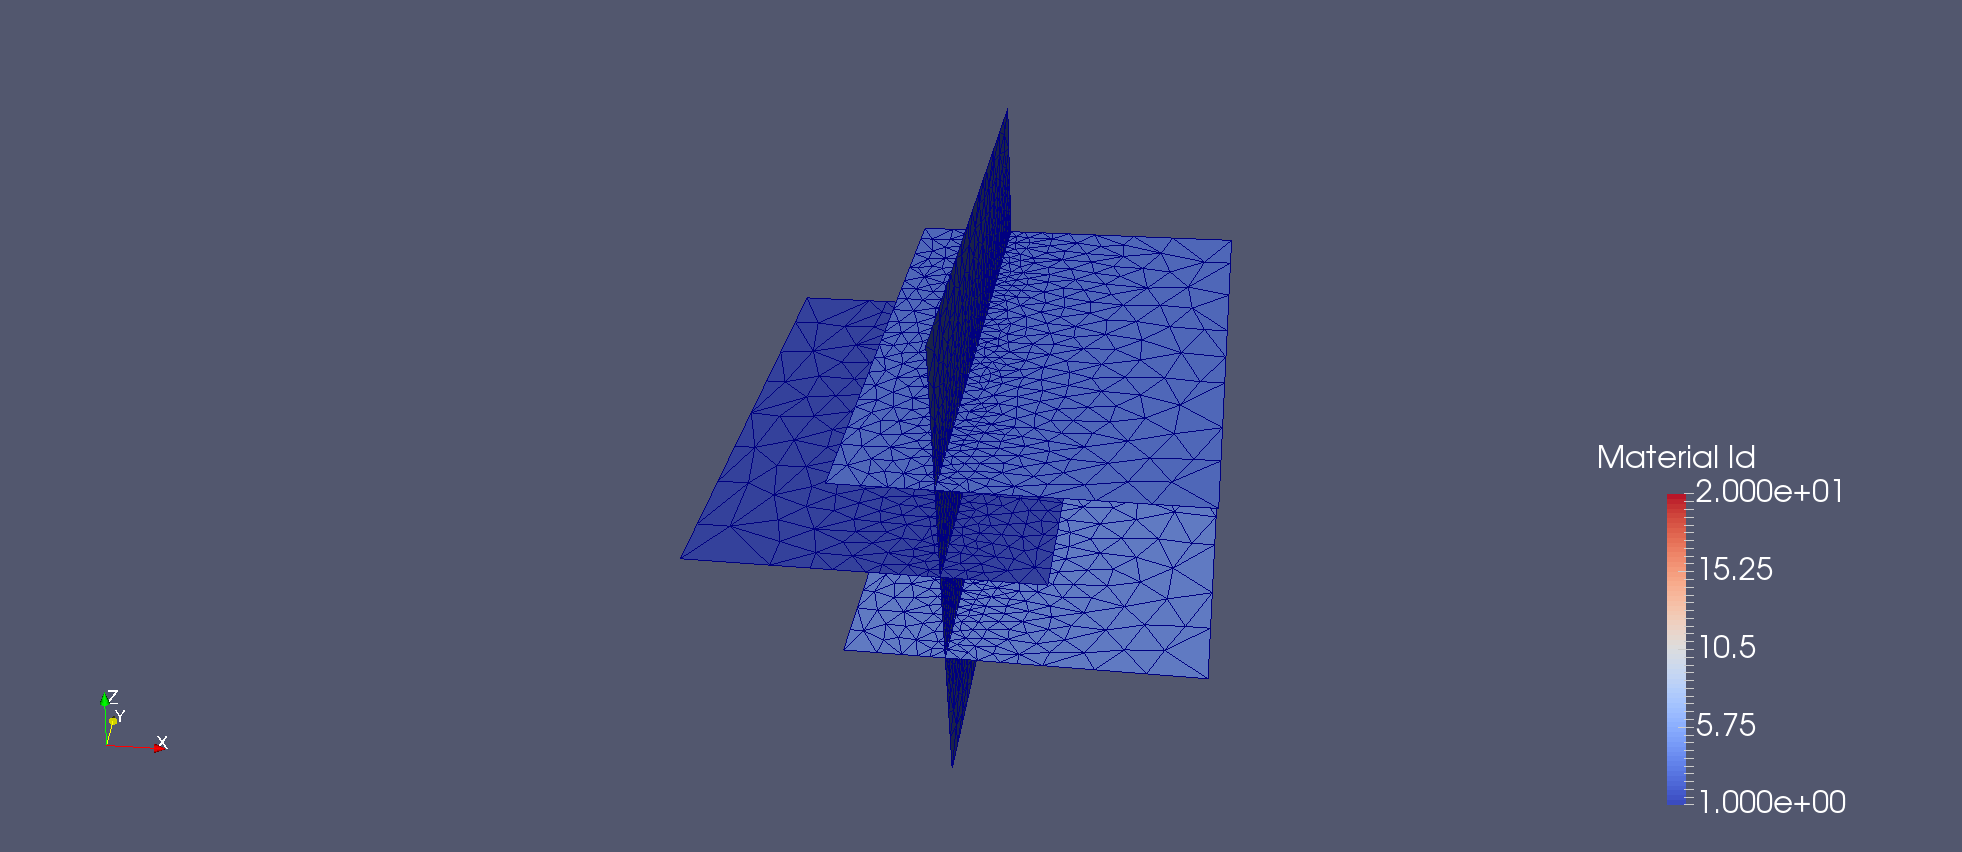
\includegraphics{4_user_rectangles_mesh.png}}\hfill}

The network of four fractures,  colored by pressure solution.
High pressure (red) Dirichlet boundary conditions are applied on the edge of the single fracture along the boundary x = -0.5, and low pressure (blue) boundary conditions are applied on the edges of the two fractures at the boundary x = 0.5.
This image is created by loading the file 4\_user\_defined\_rectangles/PFLOTRAN/parsed\_vtk/dfn\_explicit-001.vtk into Paraview.

{\hfill\scalebox{1.000000}{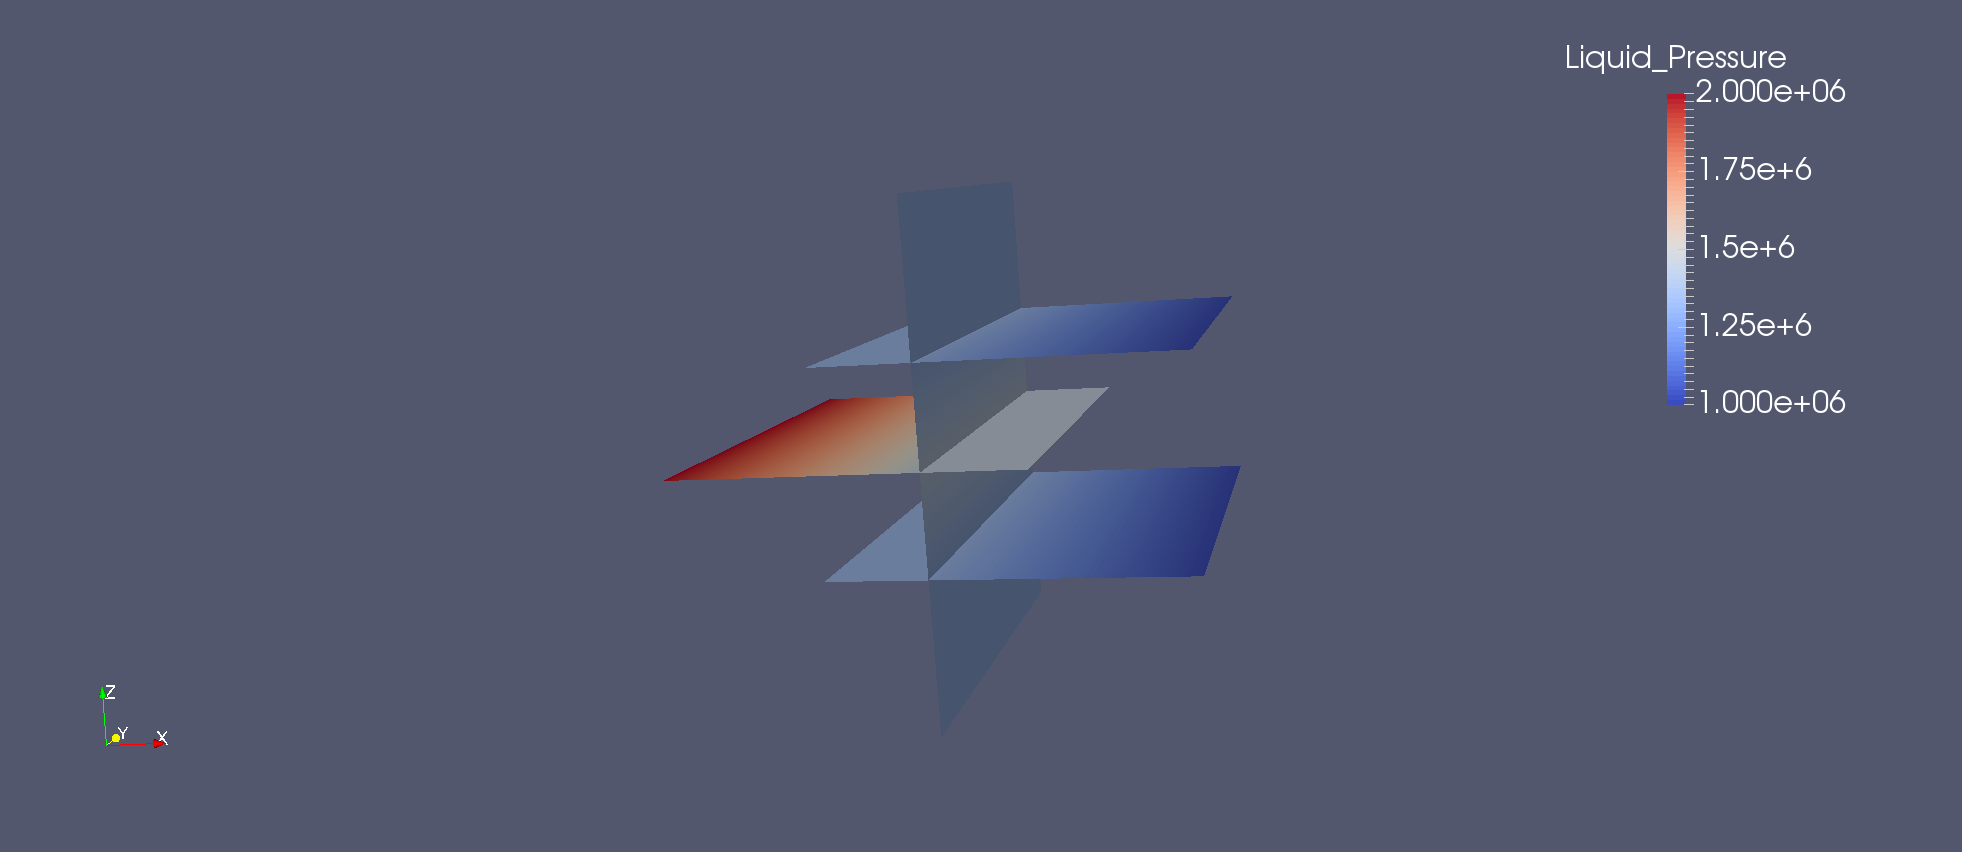
\includegraphics{4_user_rectangles_pressure.png}}\hfill}

Particle trajectories on the network of four fractures.
Particles are inserted uniformly along the inlet fracture on the left side of the image.
Particles exit the domain through the two horizontal fractures on the right side of the image.
Due to the stochastic nature of the particle tracking algorithm, your pathlines might not be exactly the same as in this image.
Trajectories are colored by the current velocity magnitude of the particle's velocity.
Trajectories can be visualized by loading the files part\_*.inp, in the folder 4\_user\_rectangles/dfnTrans/trajectories/
We have used the extract surface and tube filters in paraview for visual clarity.

{\hfill\scalebox{1.000000}{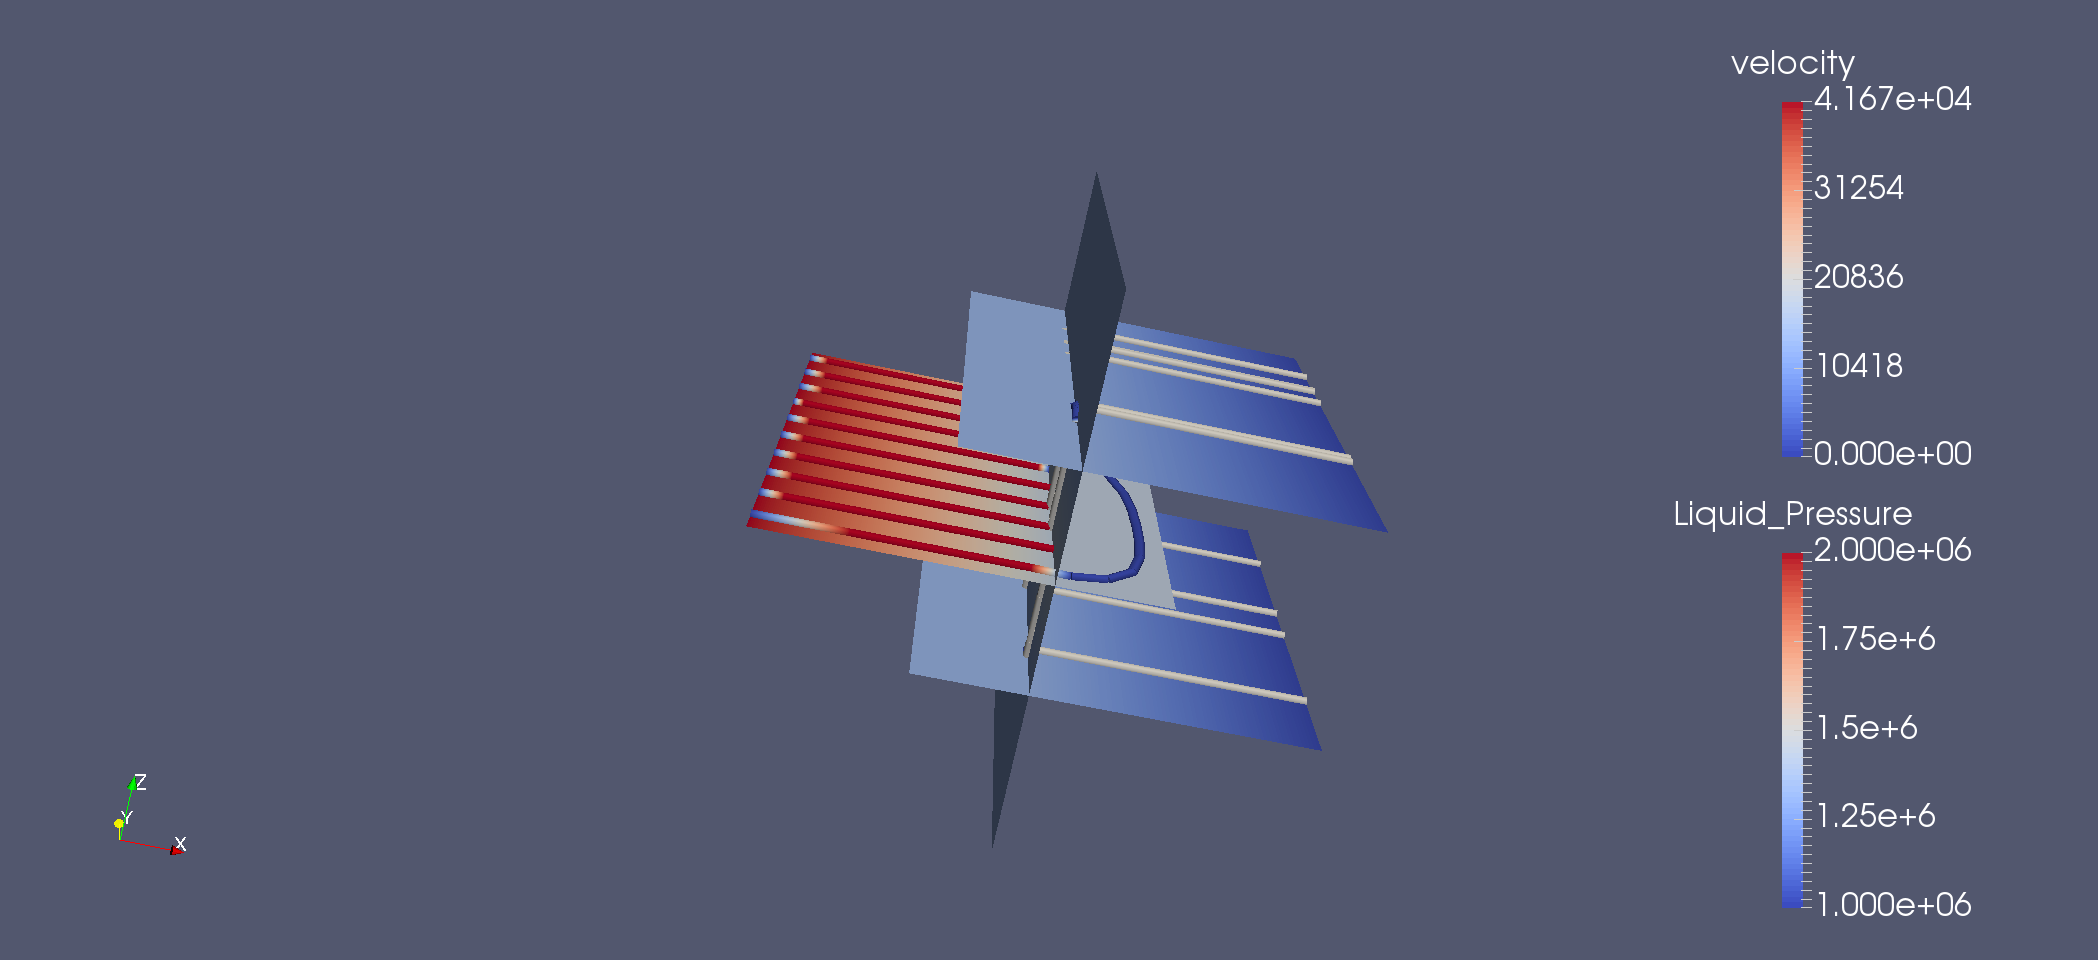
\includegraphics{4_user_rectangles_trace.png}}\hfill}

In the other tests, only a brief description and pictures are provided.


\section{4\_user\_defined\_ellipses}
\label{tutorial:user-defined-ellipses}
This test case consists of four user defined elliptical fractures within a a cubic domain with sides of length one meter. In this case the ellipses are approximated using 5 vertices. The input file specifiying the ellipses is in dfnWorks-Version2.0/tests, and is named define\_4\_user\_ellipses.dat.

{\hfill\scalebox{1.000000}{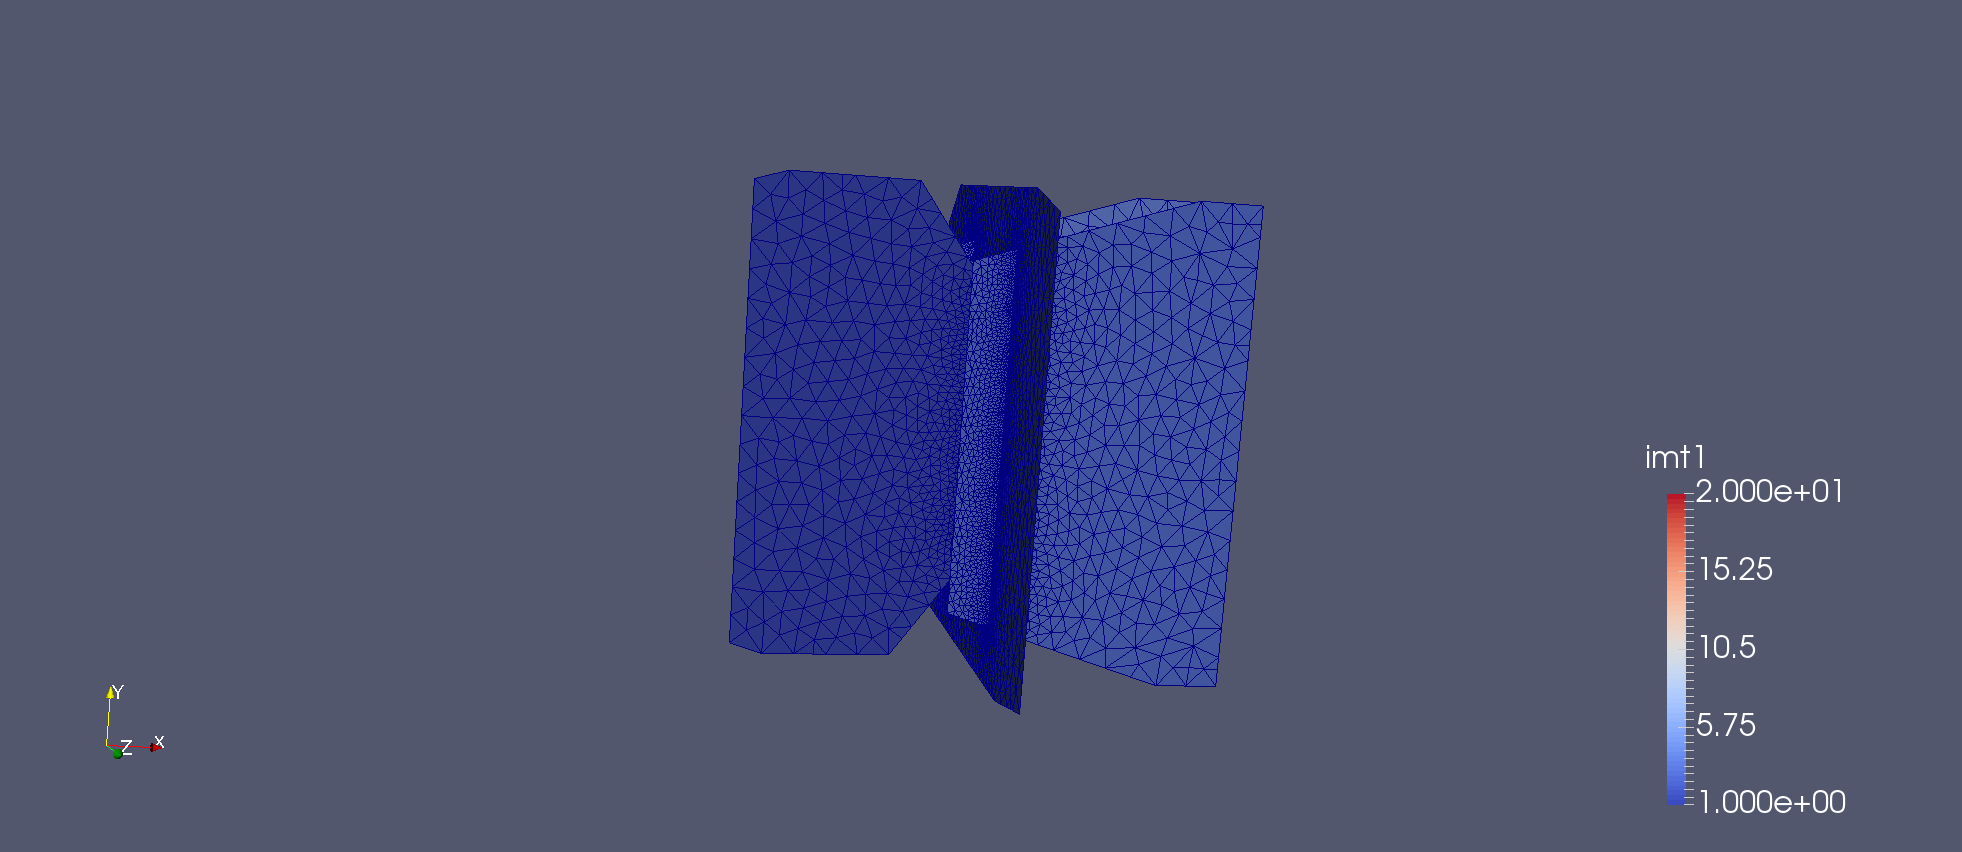
\includegraphics{4_user_ellipses_mesh.png}}\hfill}

\begin{DUlineblock}{0em}
\item[] 
\item[] 
\end{DUlineblock}

{\hfill\scalebox{1.000000}{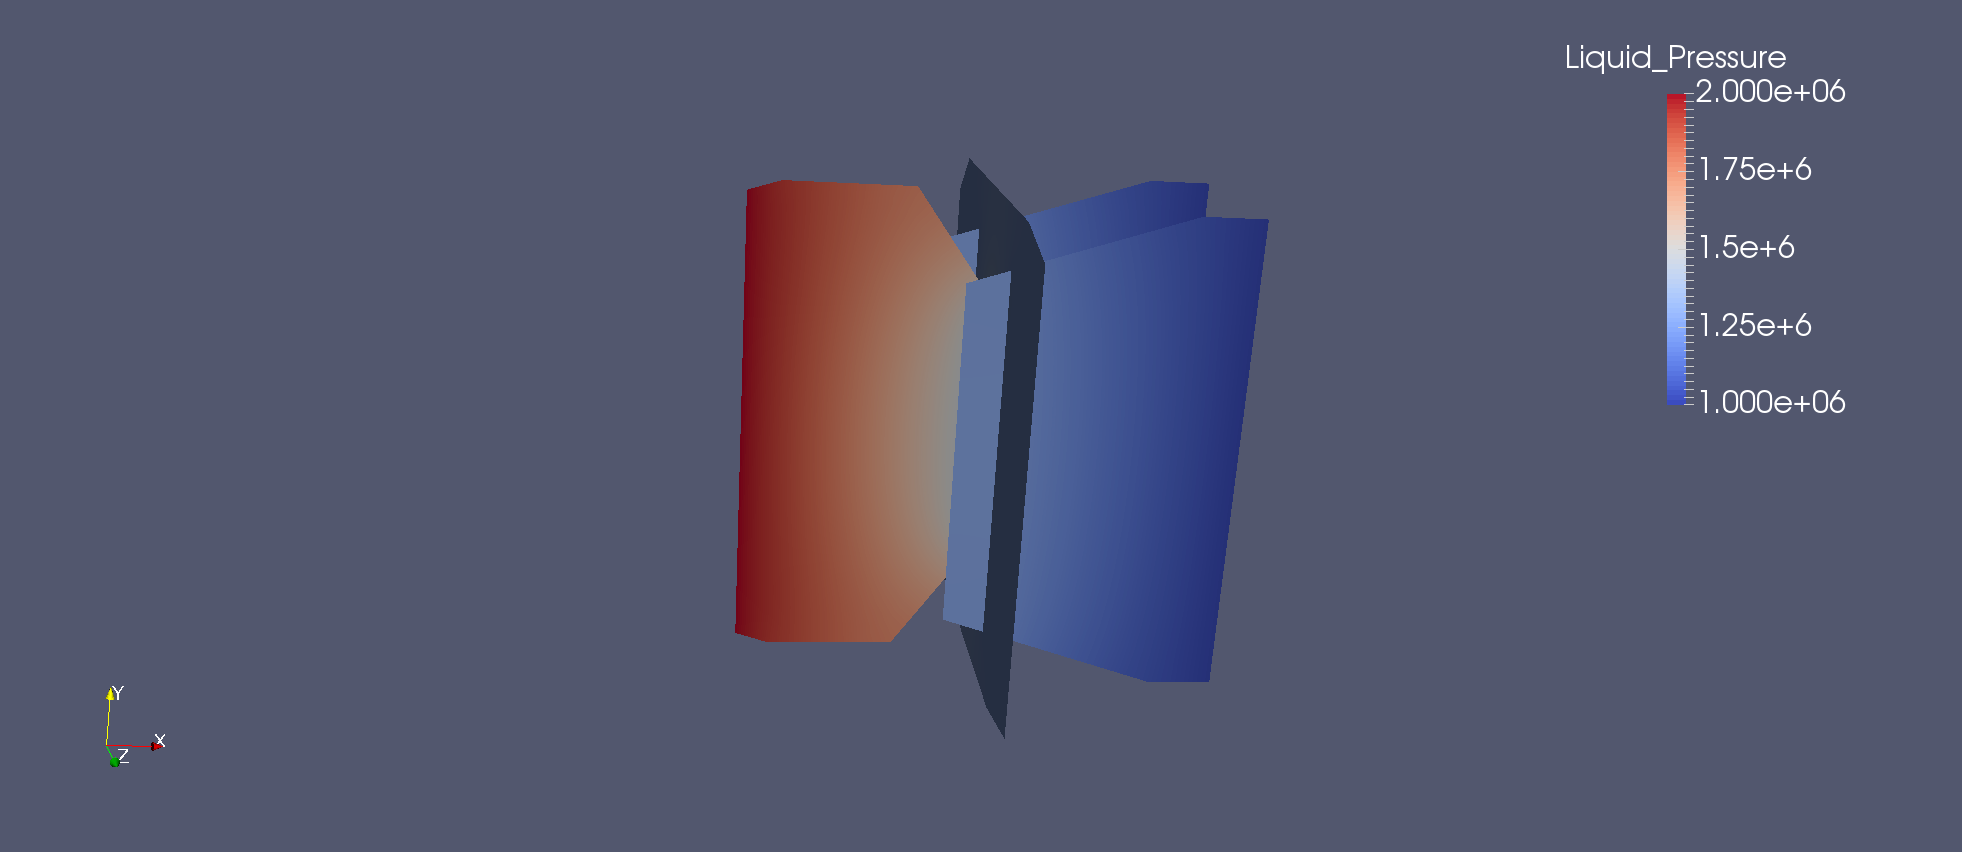
\includegraphics{4_user_ellipses_pressure.png}}\hfill}

\begin{DUlineblock}{0em}
\item[] 
\item[] 
\end{DUlineblock}

{\hfill\scalebox{1.000000}{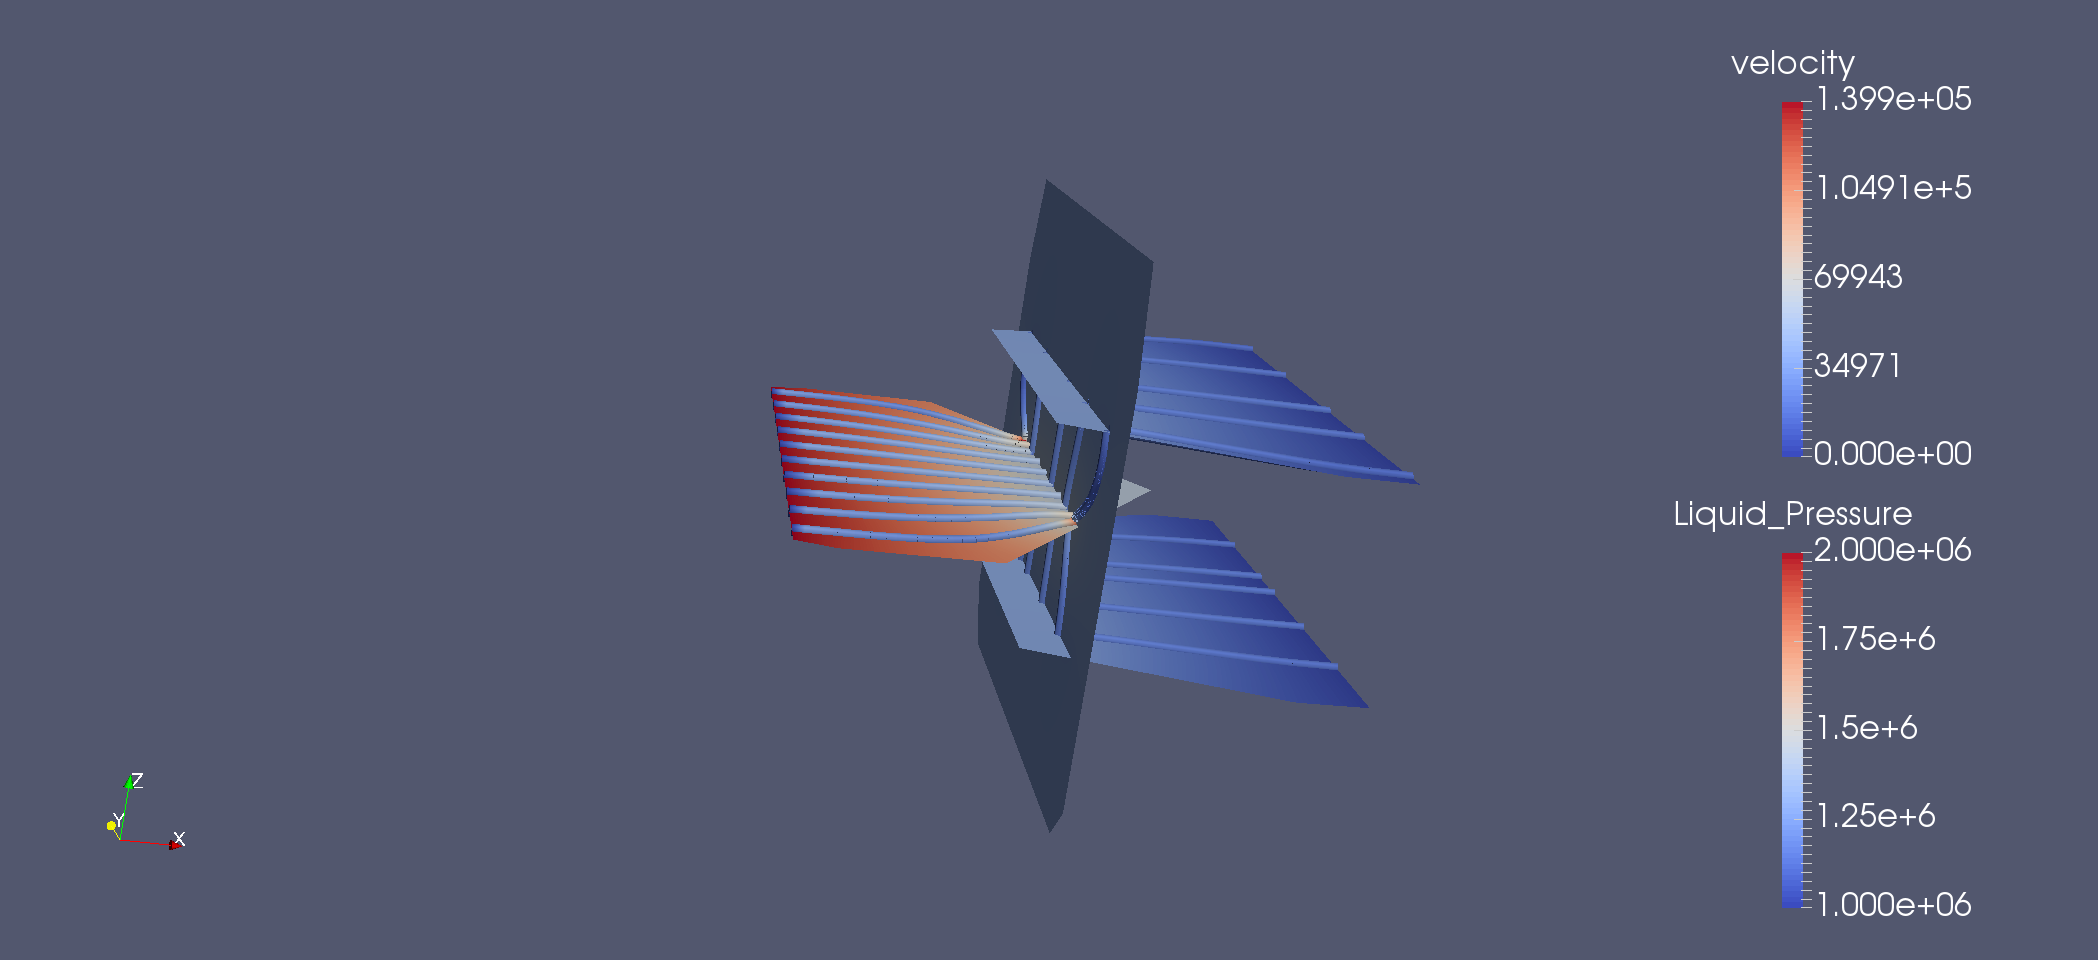
\includegraphics{4_user_ellipses_trace.png}}\hfill}

\begin{DUlineblock}{0em}
\item[] 
\item[] 
\end{DUlineblock}


\section{truncated\_power\_law\_dist}
\label{tutorial:truncated-power-law-dist}
This test case consists of two families whose sizes have a truncated power law distribution with a minimum size of 0.5m and a maximum size of 50m. The domain size is cubic with an edge length of 4m. The other input parameters can be found in tests/gen\_truncated\_power\_law\_dist.dat.

{\hfill\scalebox{1.000000}{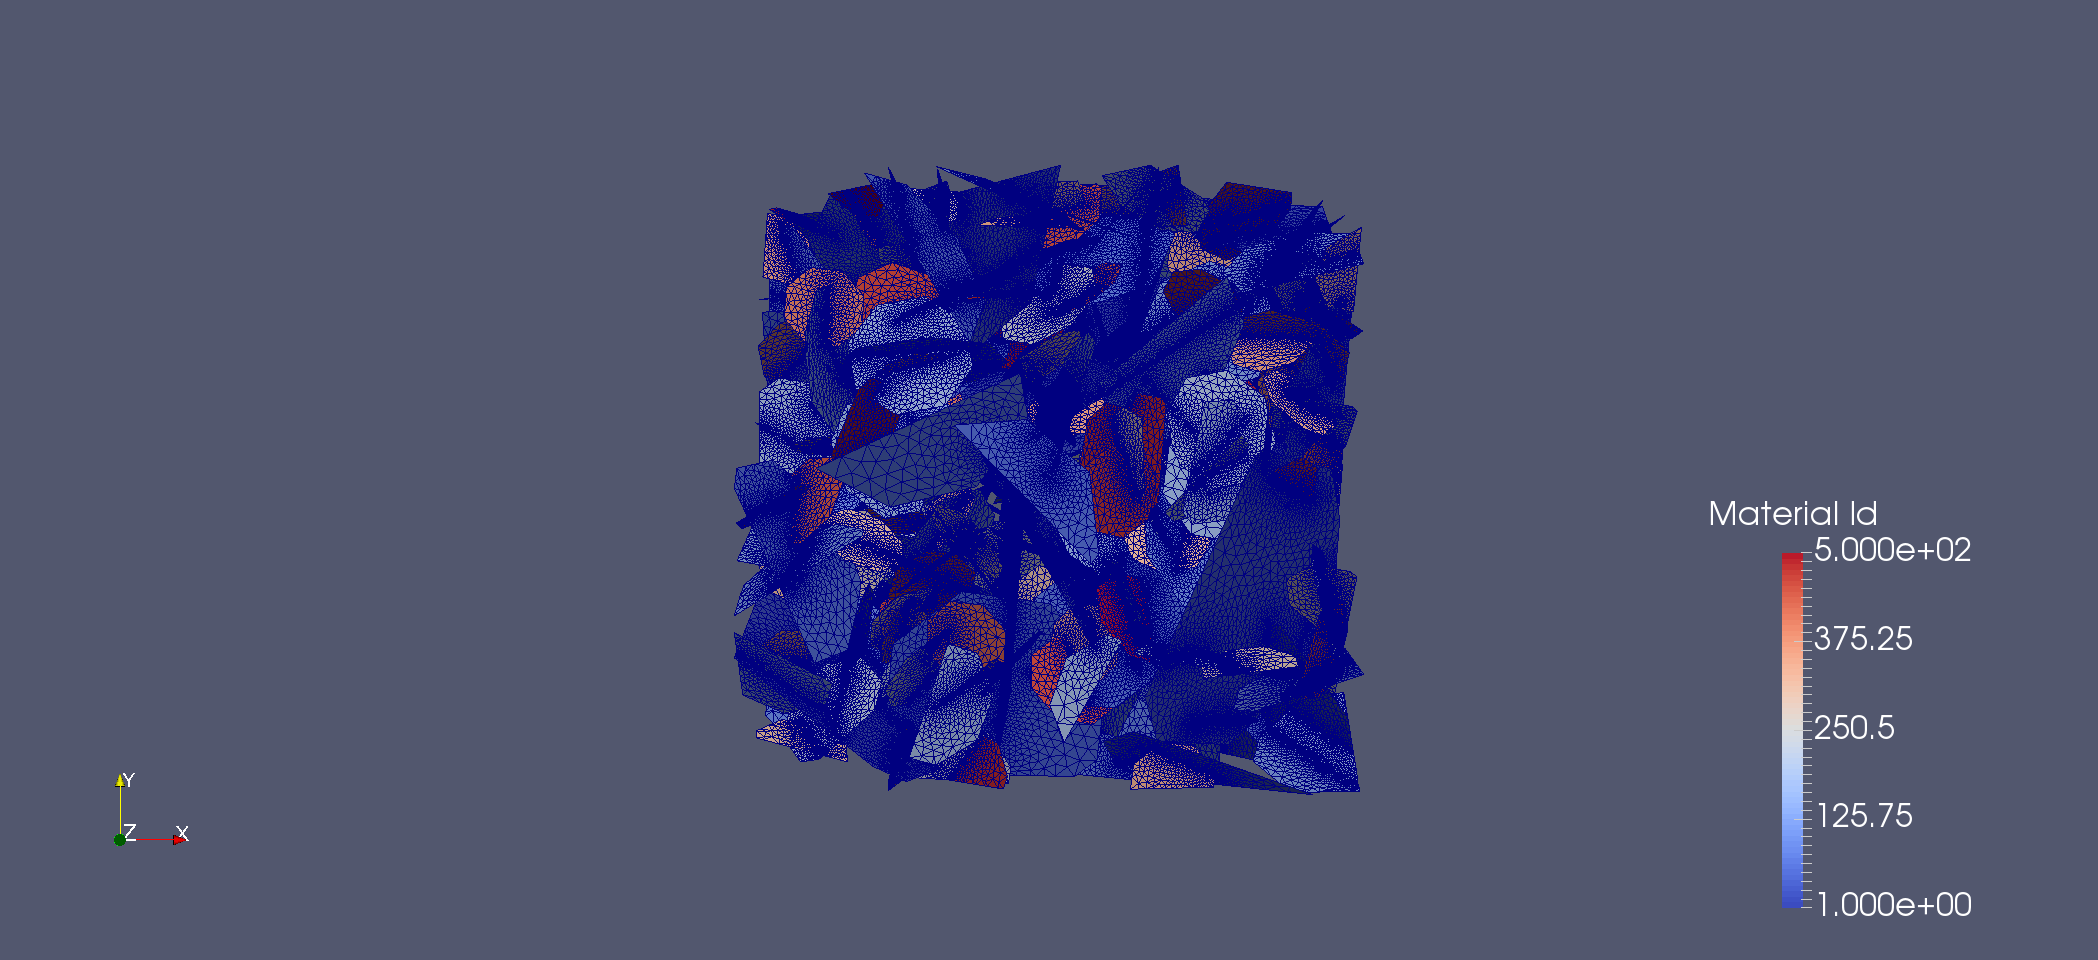
\includegraphics{power_mesh.png}}\hfill}

\begin{DUlineblock}{0em}
\item[] 
\item[] 
\end{DUlineblock}

{\hfill\scalebox{1.000000}{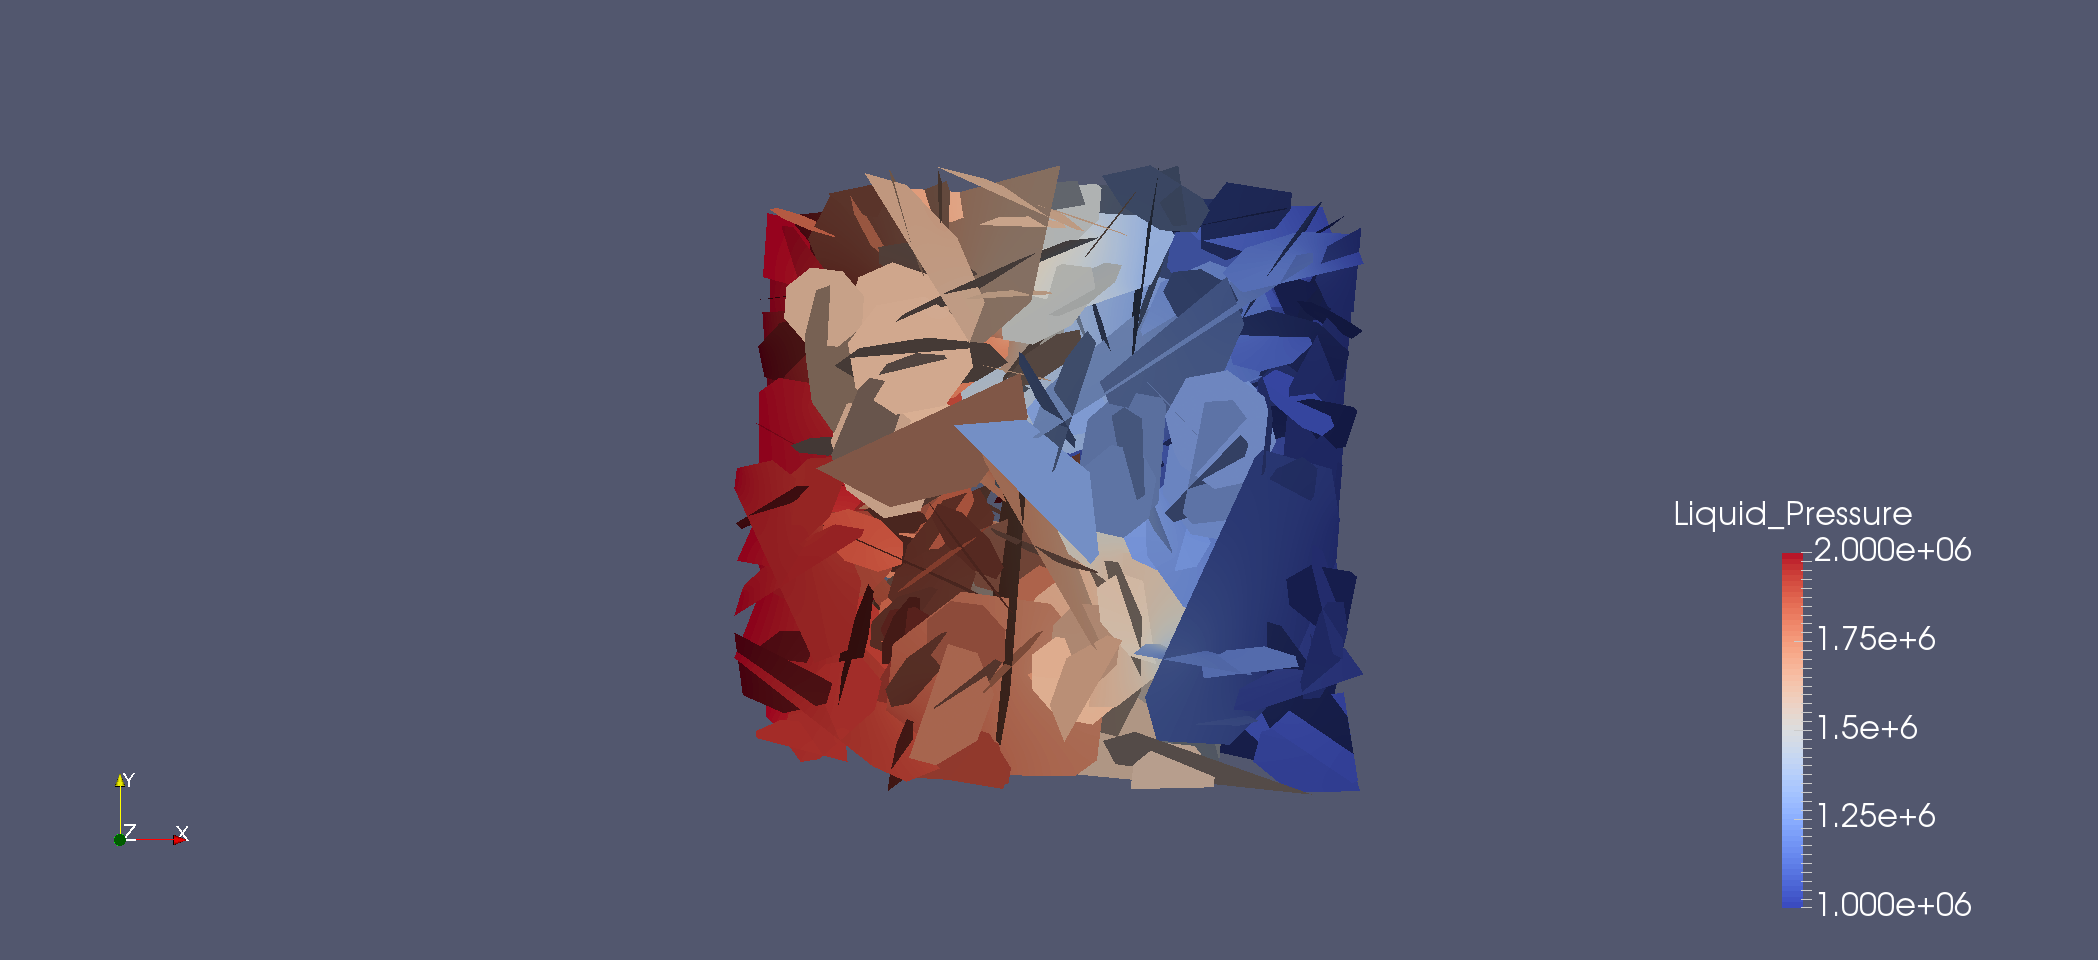
\includegraphics{power_pressure.png}}\hfill}

\begin{DUlineblock}{0em}
\item[] 
\item[] 
\end{DUlineblock}

{\hfill\scalebox{1.000000}{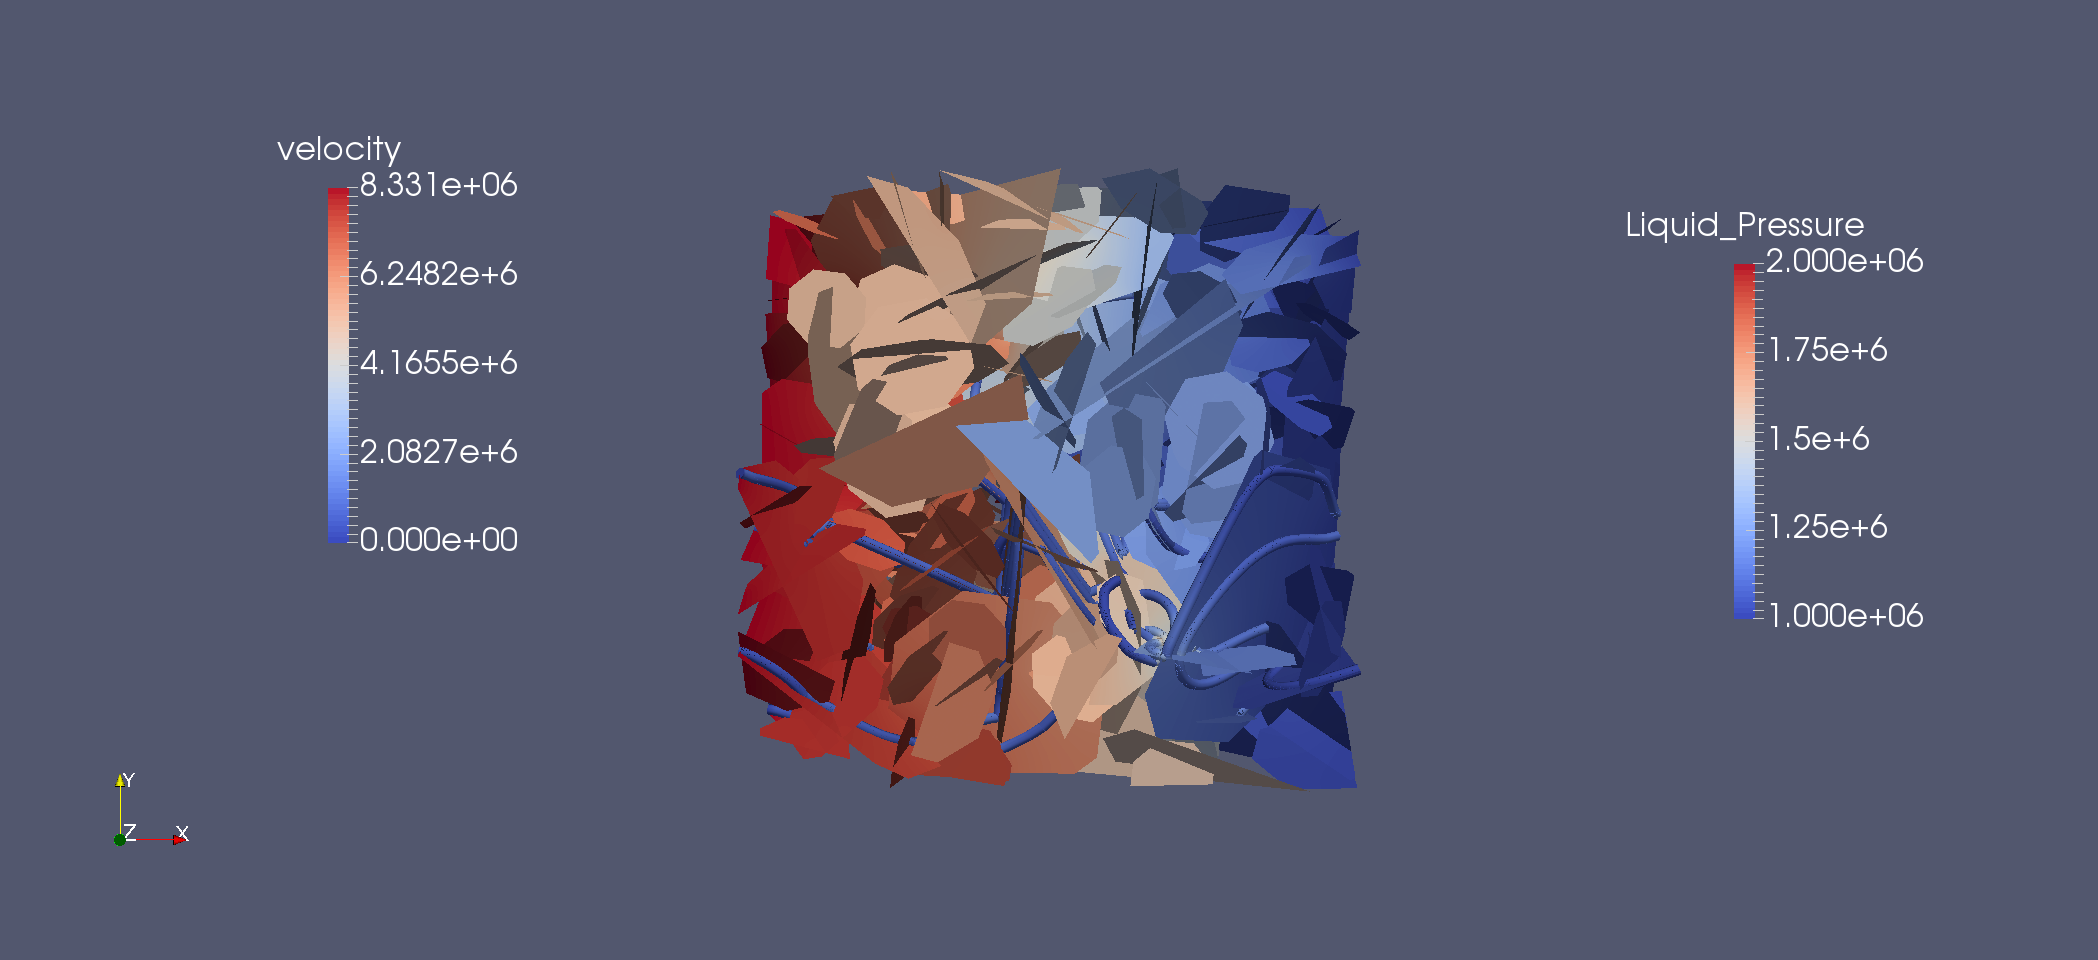
\includegraphics{power_trace.png}}\hfill}


\section{exponential\_dist}
\label{tutorial:exponential-dist}
This test case consists of a family of fractures whose size is exponentially distributed with a minimum size of 1m and a maximum size of 50m. The domain is cubic with an edge length of 10m. All input parameters for the generator can be found in tests/gen\_exponential\_dist.dat.

{\hfill\scalebox{1.000000}{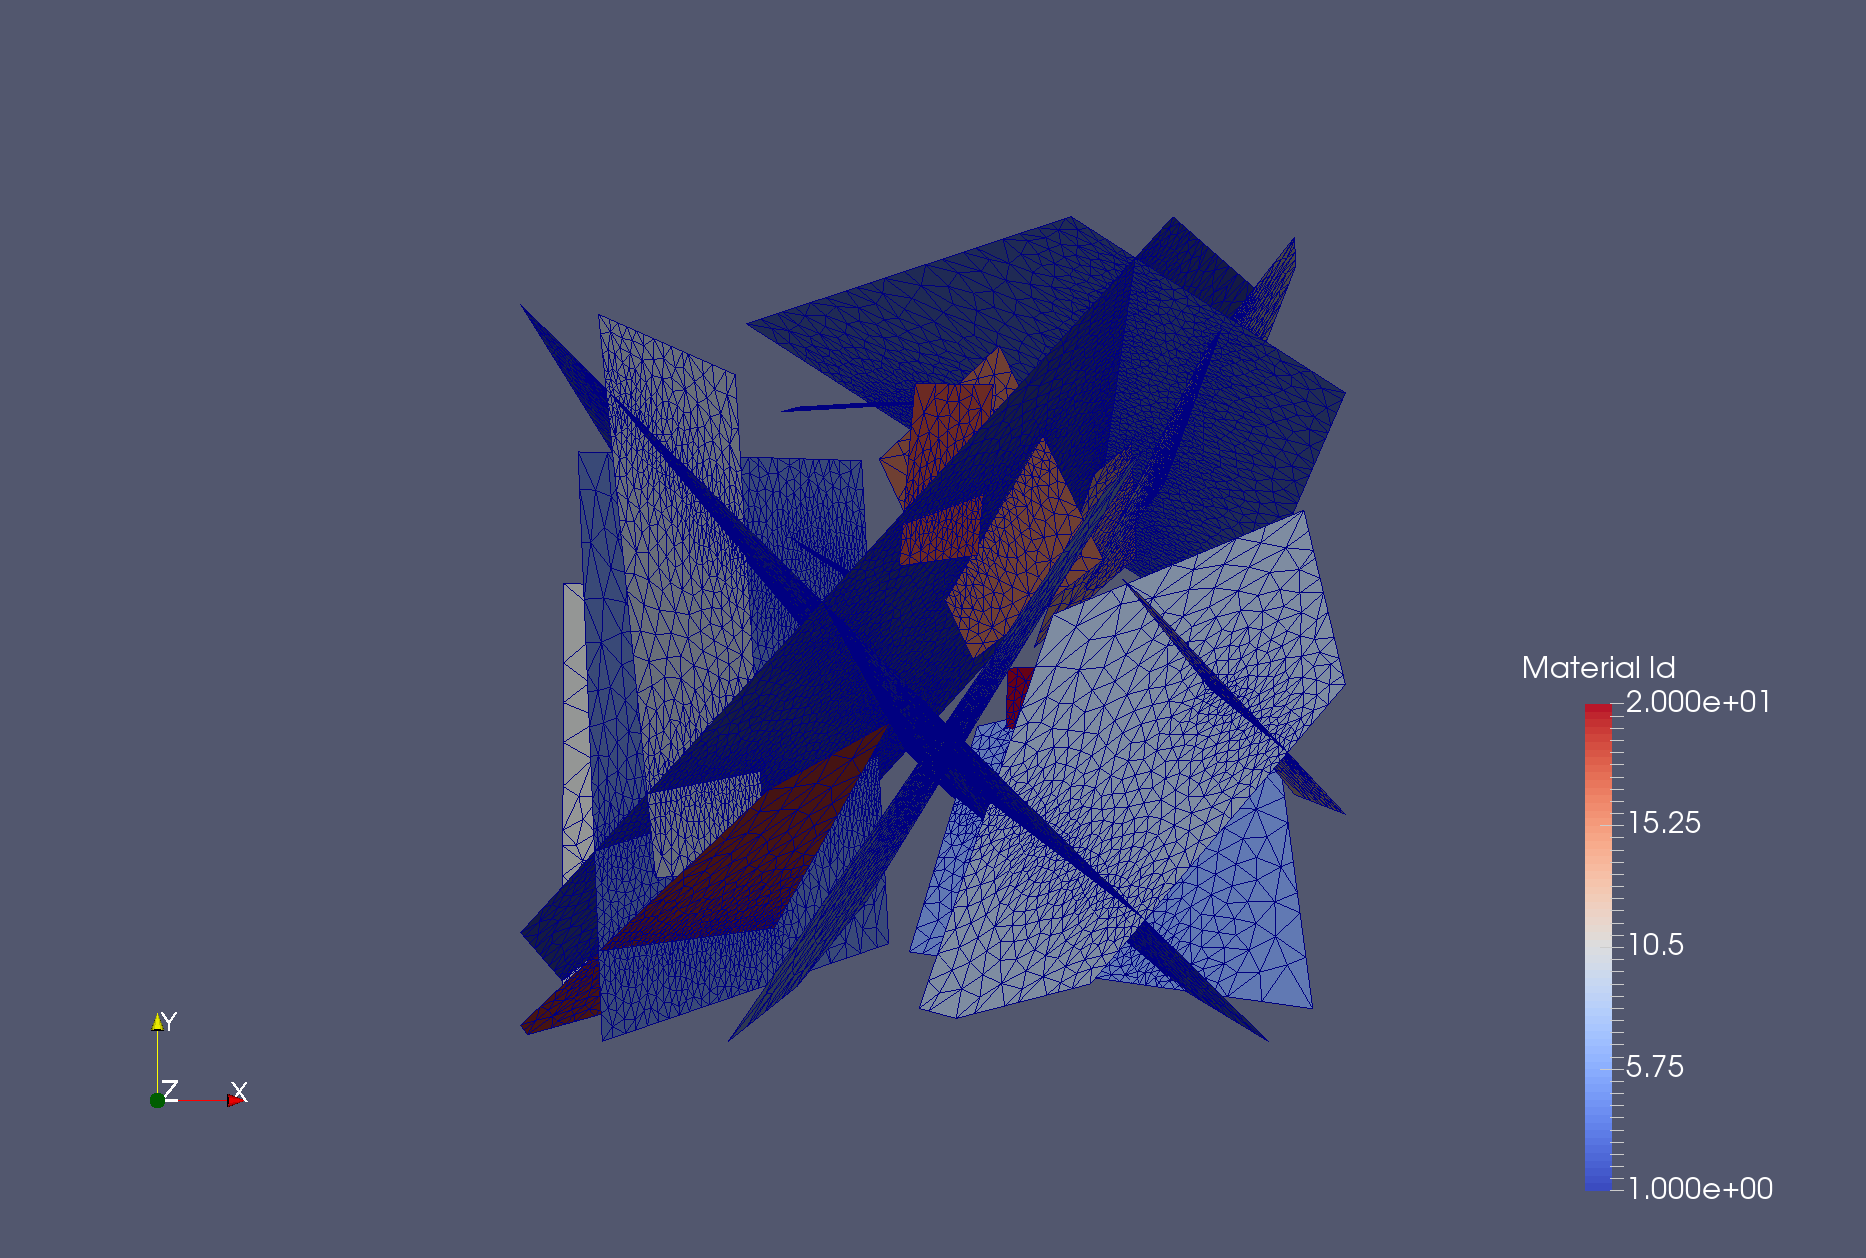
\includegraphics{exp_mesh.png}}\hfill}

\begin{DUlineblock}{0em}
\item[] 
\item[] 
\end{DUlineblock}

{\hfill\scalebox{1.000000}{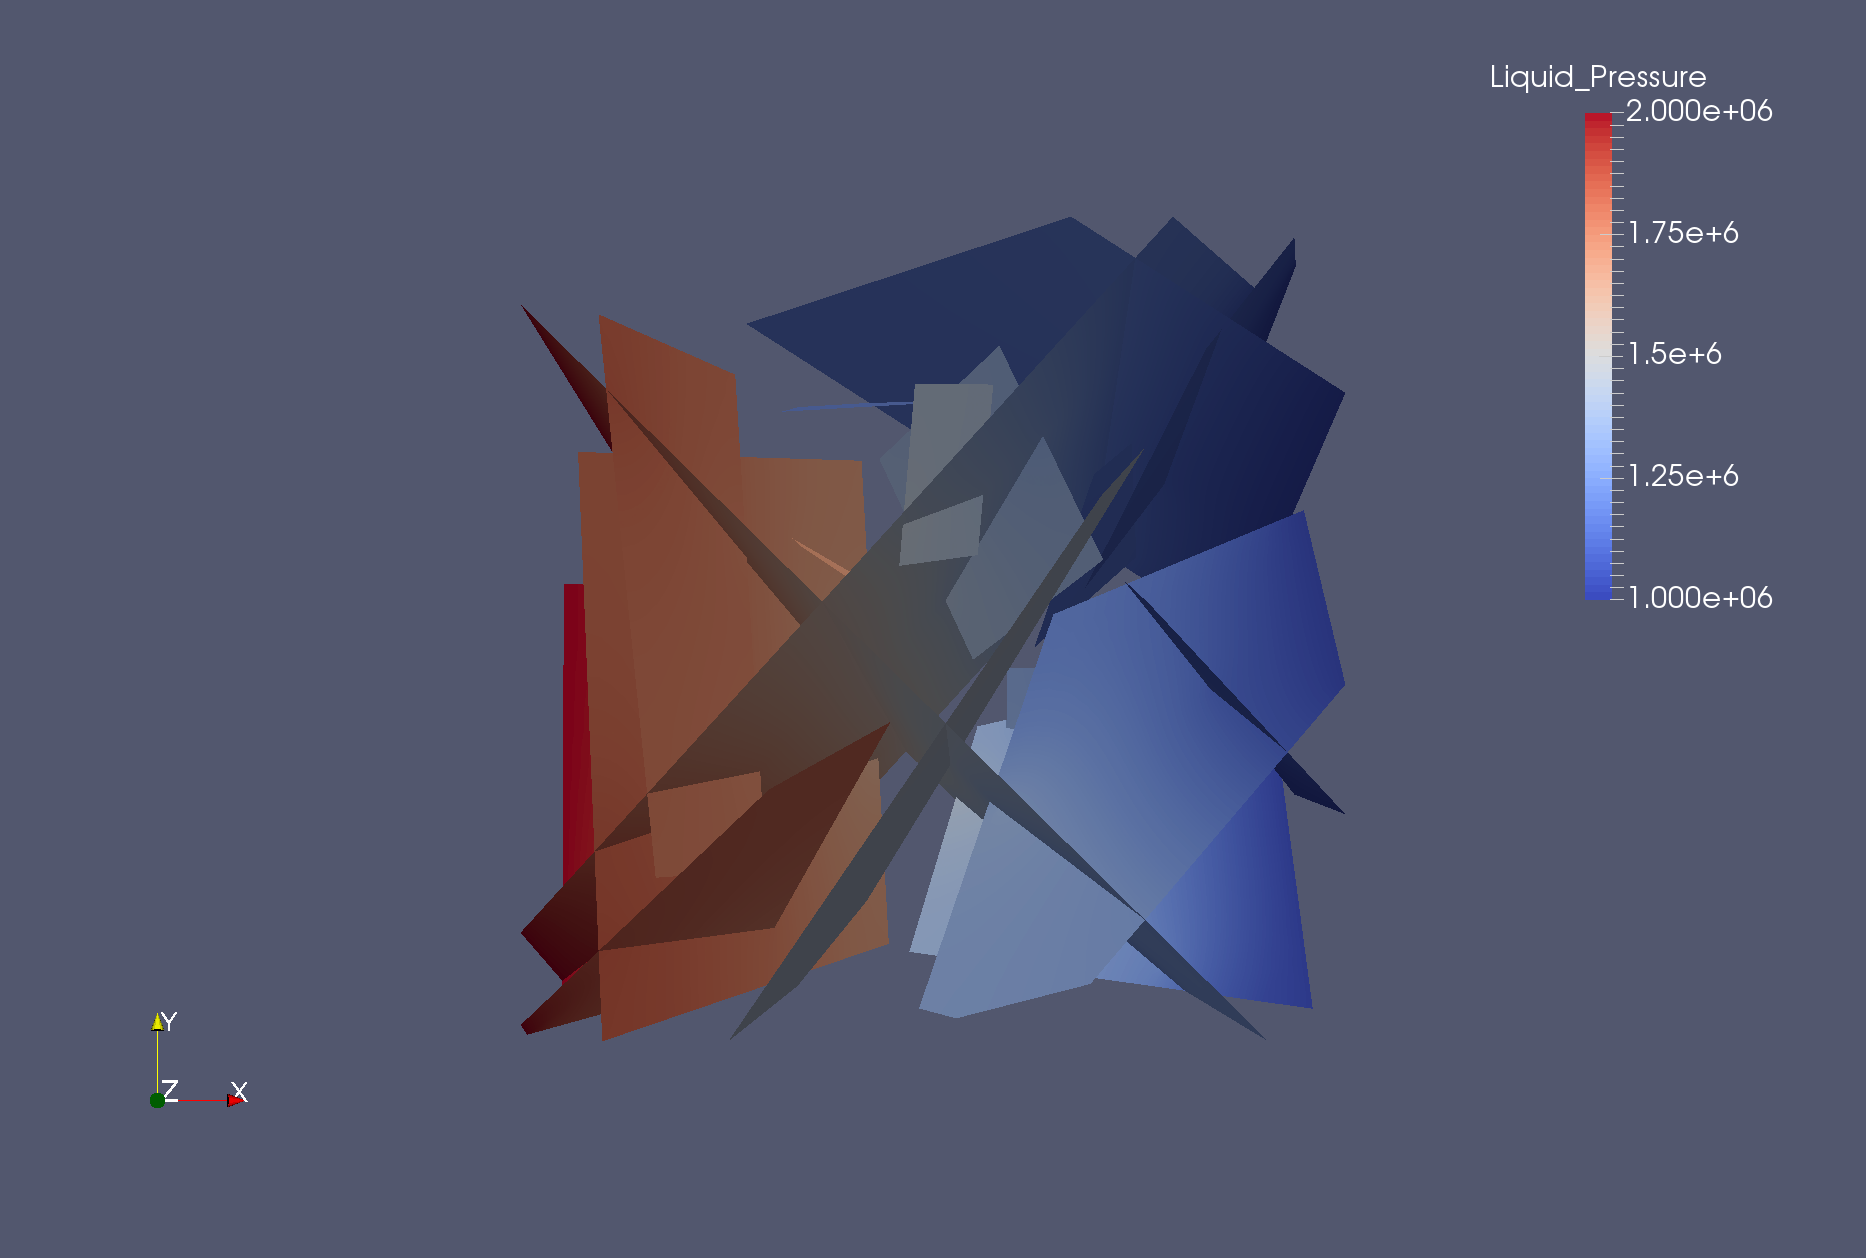
\includegraphics{exp_pressure.png}}\hfill}

\begin{DUlineblock}{0em}
\item[] 
\item[] 
\end{DUlineblock}

{\hfill\scalebox{1.000000}{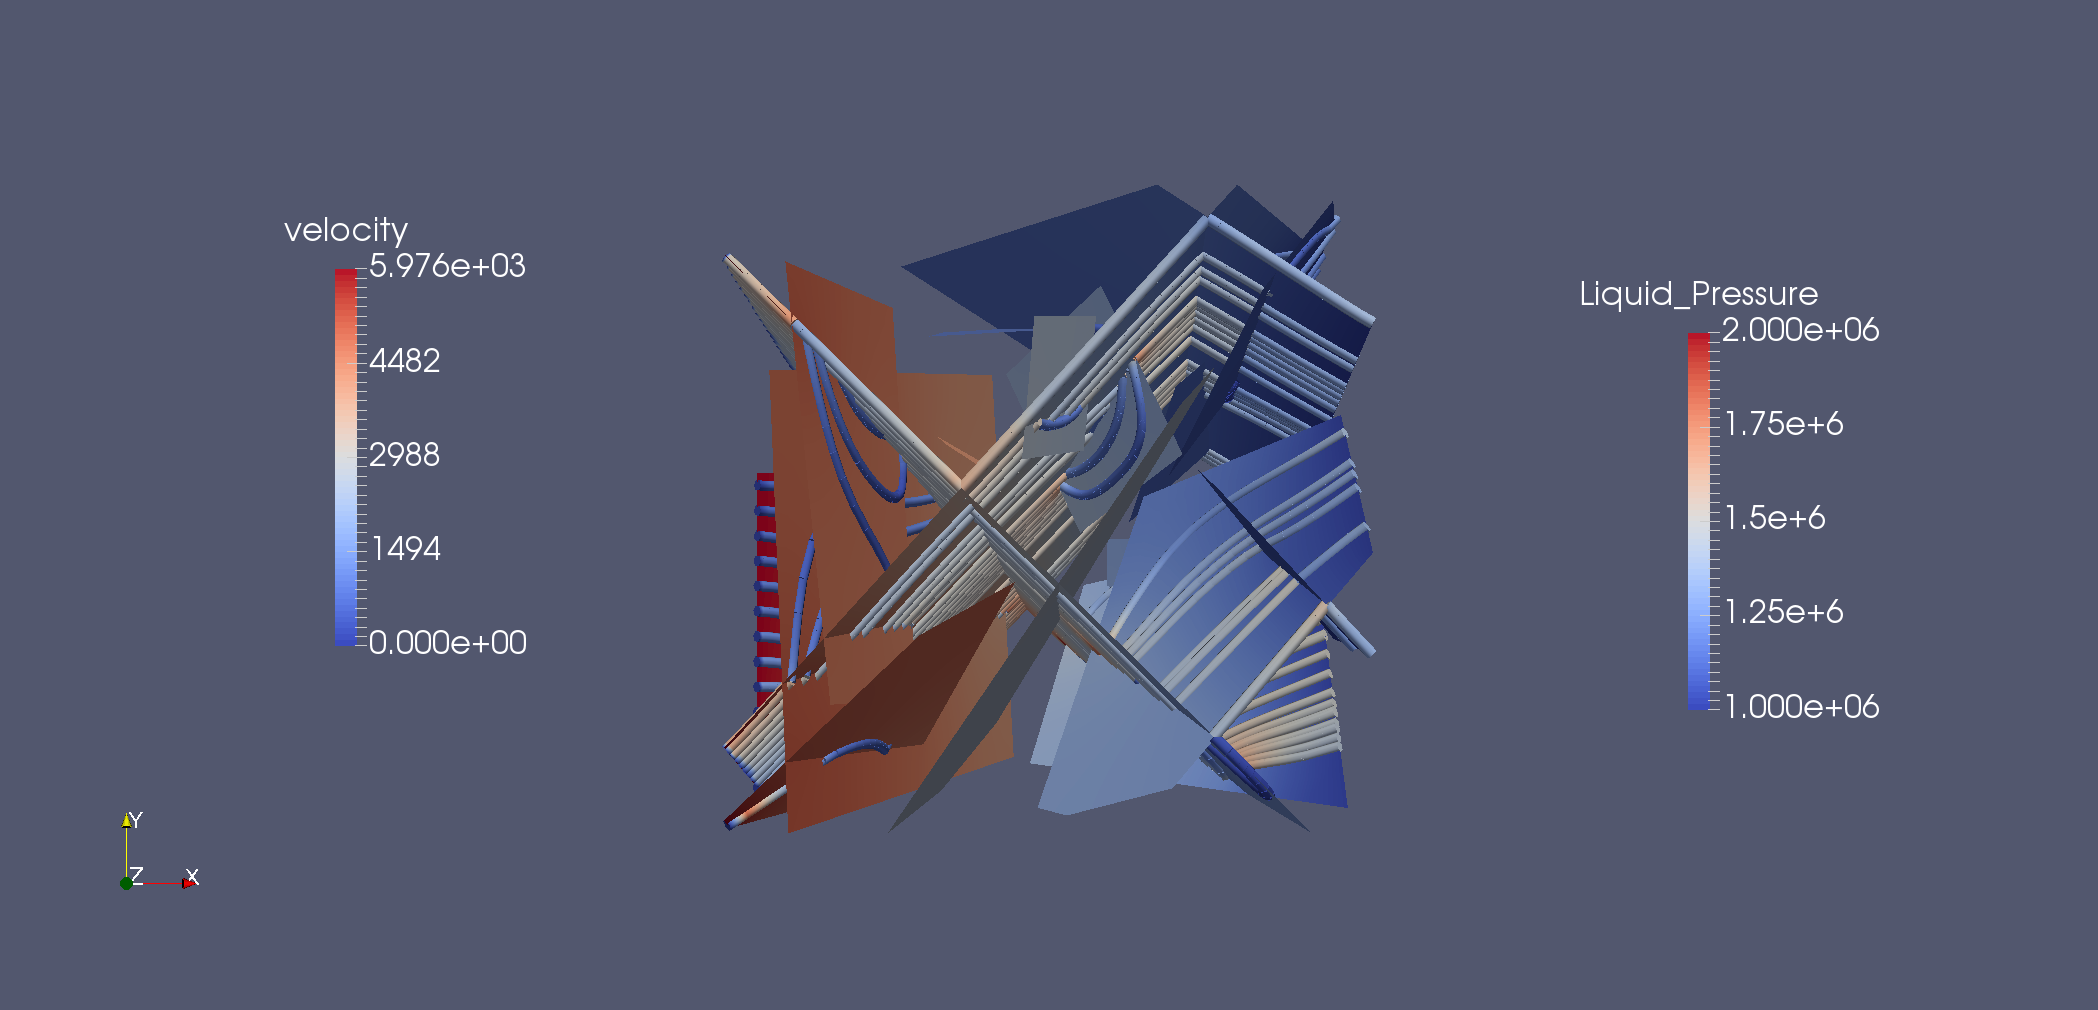
\includegraphics{exp_trace.png}}\hfill}

\begin{DUlineblock}{0em}
\item[] 
\item[] 
\end{DUlineblock}


\section{lognormal\_dist}
\label{tutorial:lognormal-dist}
This test case consists of two fracture families whose sizes have a lognormal distribution with a minimum size of 0.5m and a maximum size of 50m. The domain size is cubic with an edge length of 10m. All input parameters for the generator can be found in tests/gen\_lognormal\_dist.dat.

{\hfill\scalebox{1.000000}{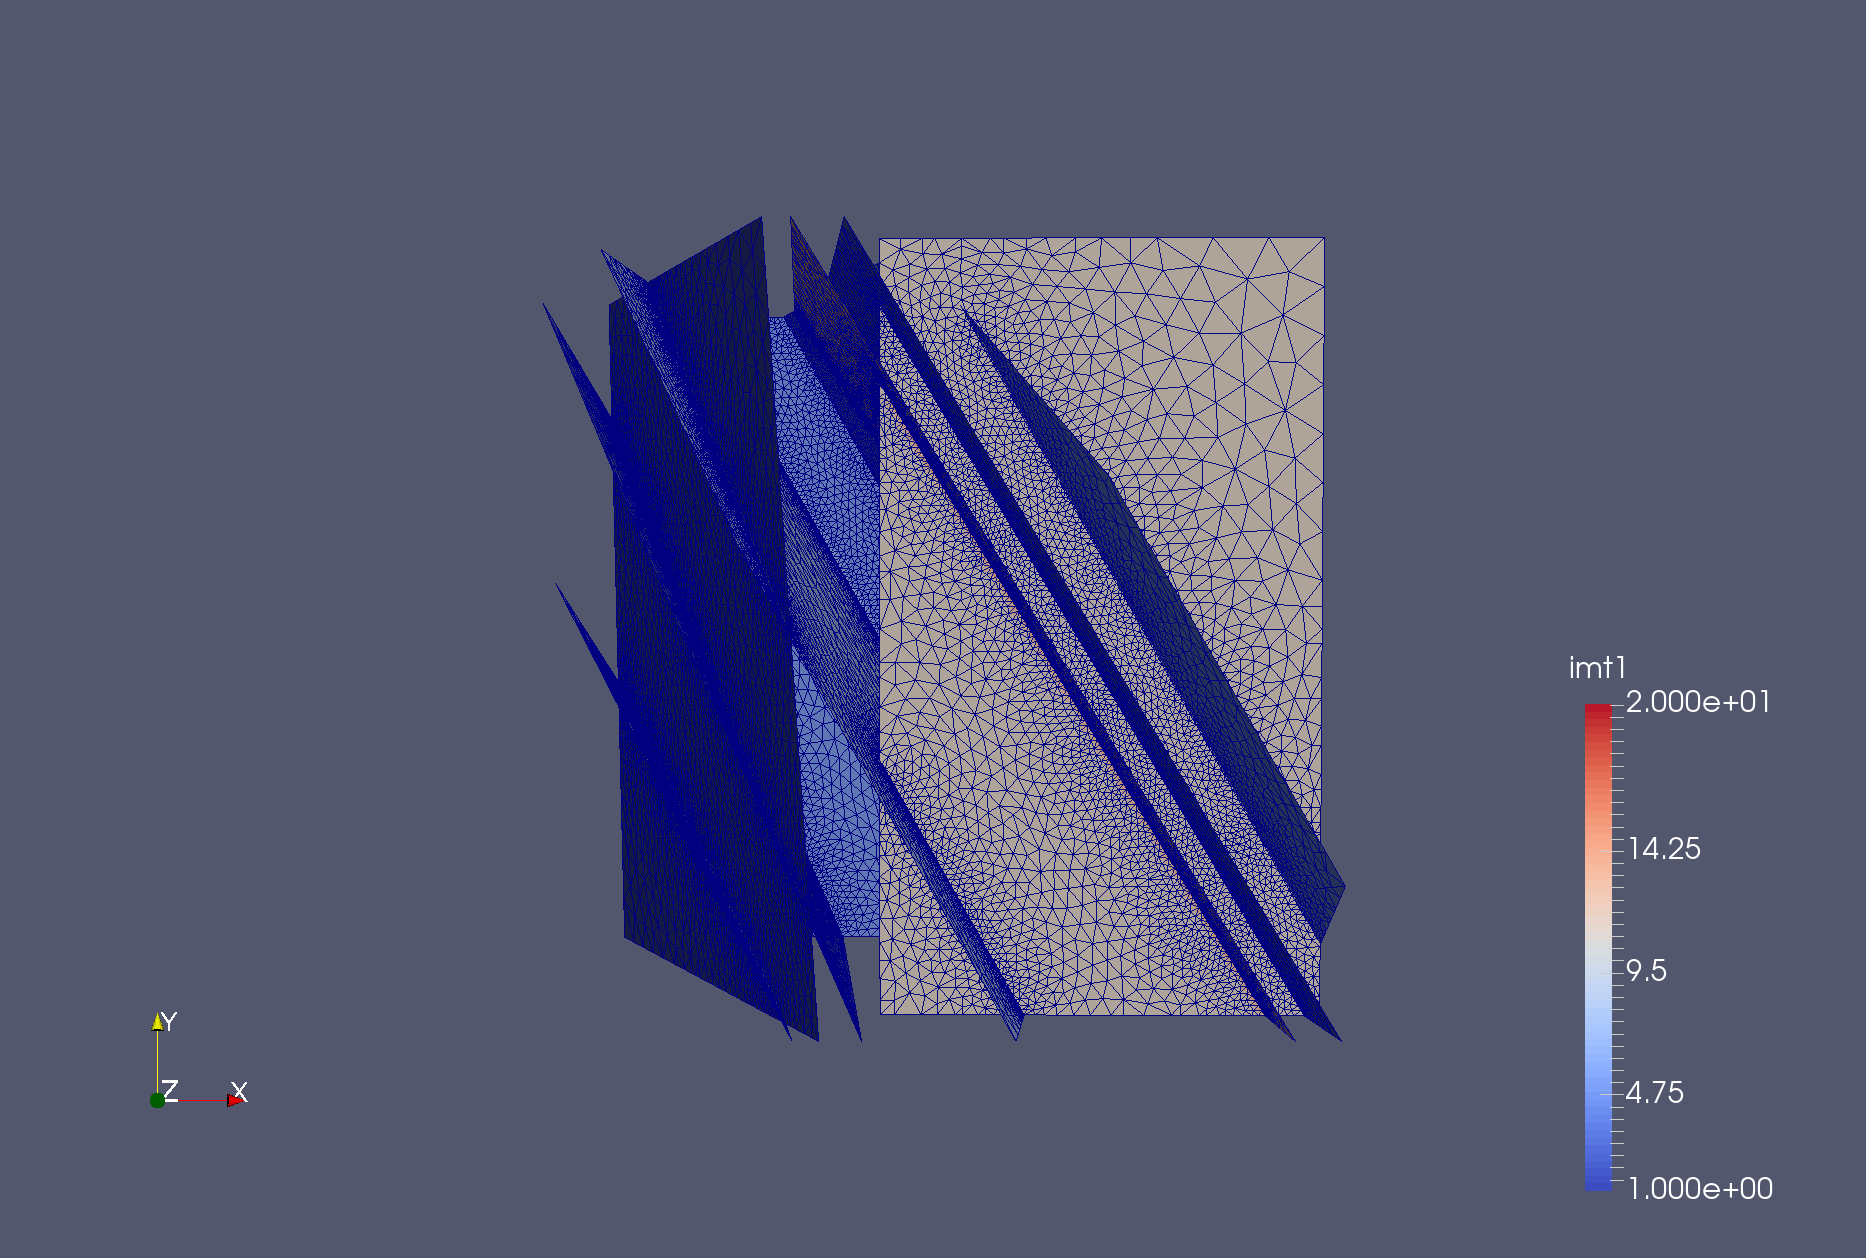
\includegraphics{lognormal_mesh.png}}\hfill}

\begin{DUlineblock}{0em}
\item[] 
\item[] 
\end{DUlineblock}

{\hfill\scalebox{1.000000}{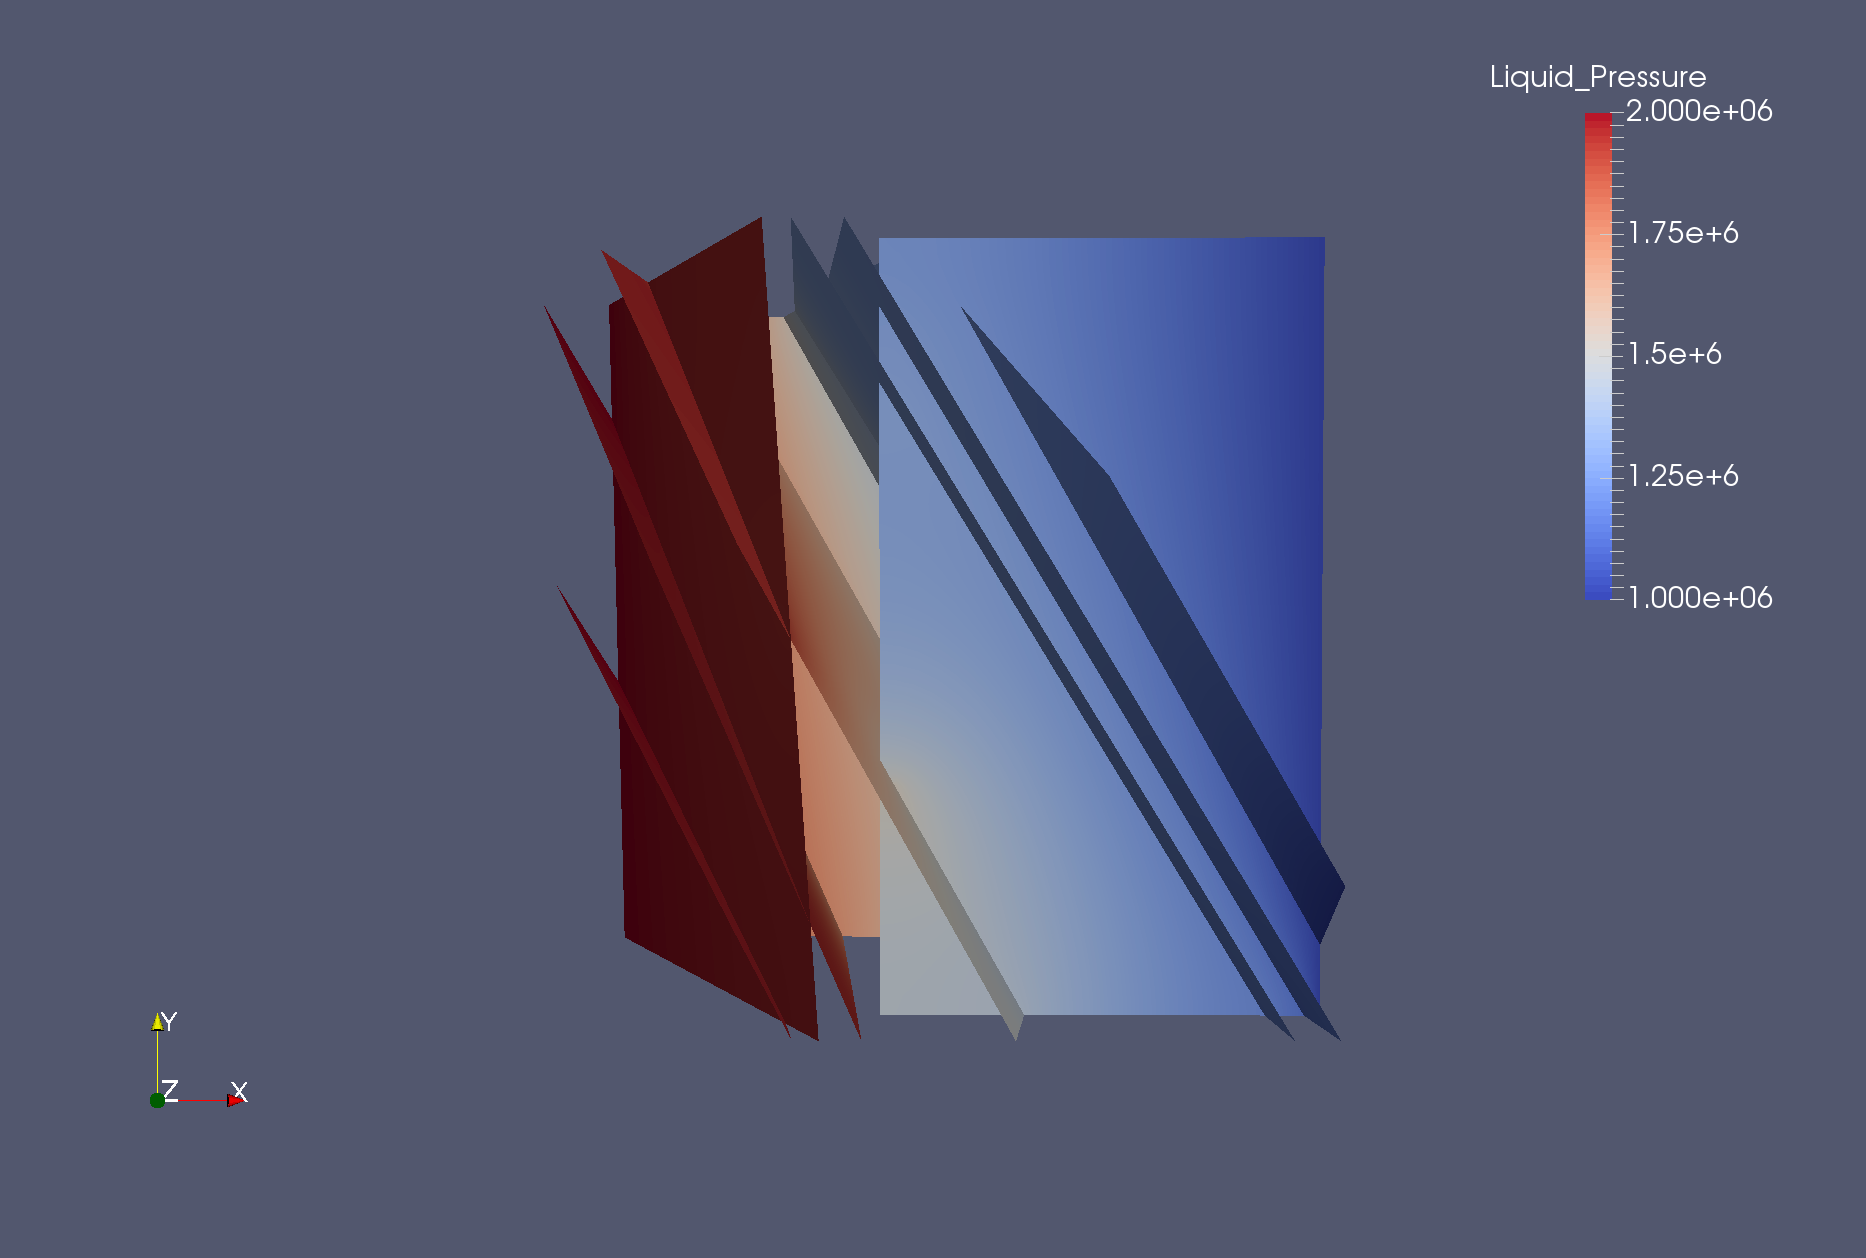
\includegraphics{lognormal_pressure.png}}\hfill}

\begin{DUlineblock}{0em}
\item[] 
\item[] 
\end{DUlineblock}

{\hfill\scalebox{1.000000}{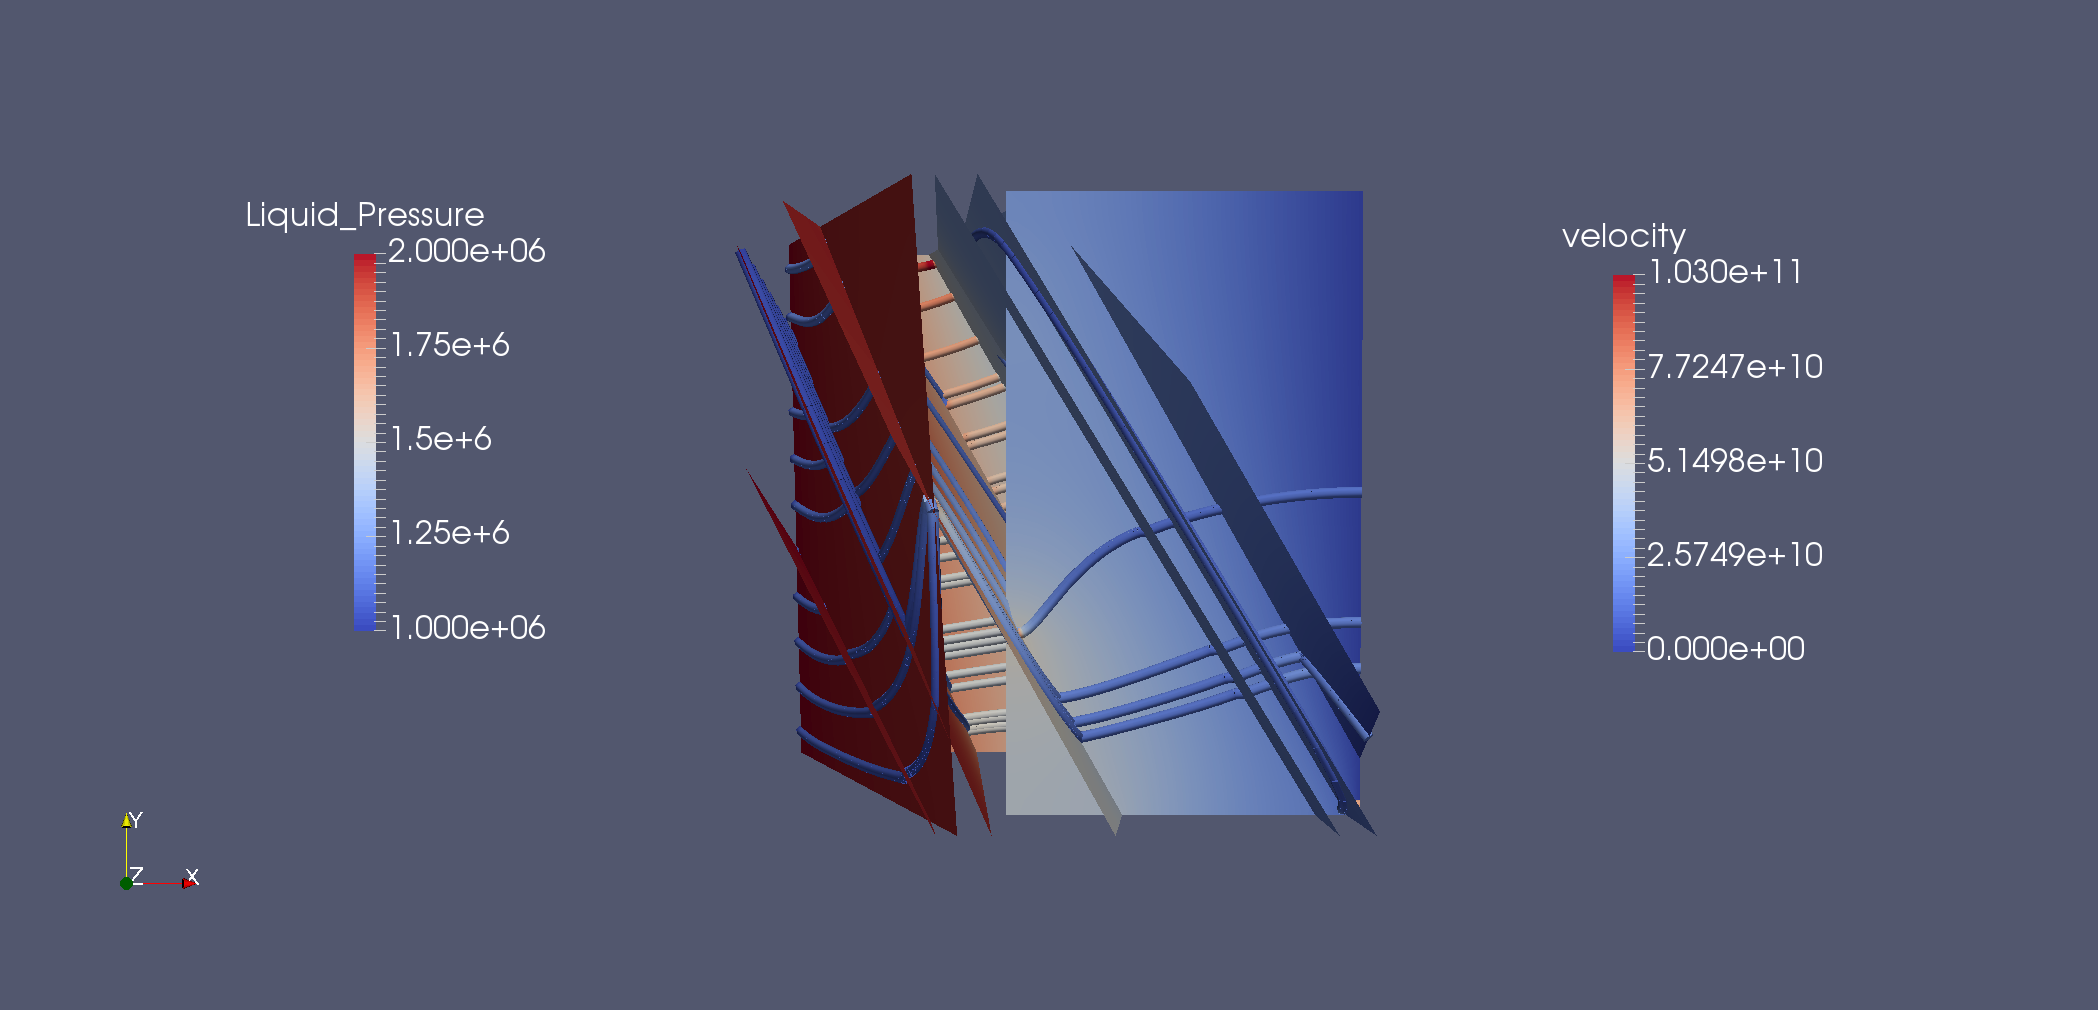
\includegraphics{lognormal_trace.png}}\hfill}

\begin{DUlineblock}{0em}
\item[] 
\item[] 
\end{DUlineblock}


\chapter{Example Applications}
\label{applications:applications-chapter}\label{applications::doc}\label{applications:example-applications}

\section{Carbon dioxide sequestration}
\label{applications:carbon-dioxide-sequestration}
DFNWORKS provides the framework necessary to perform multiphase simulations (such as flow and reactive transport) at the reservoir scale. A particular application, highlighted here, is sequestering CO2 from anthropogenic sources and disposing it in geological formations such as deep saline aquifers and abandoned oil fields. Geological CO2 sequestration is one of the principal methods under consideration to reduce carbon footprint in the atmosphere due to fossil fuels (Bachu, 2002; Pacala and Socolow, 2004). For safe and sustainable long-term storage of CO2 and to prevent leaks through existing faults and fractured rock (along with the ones created during the injection process), understanding the complex physical and chemical interactions between CO2, water (or brine) and fractured rock, is vital. DFNWORKS capability to study multiphase flow in a DFN can be used to study potential CO2 migration through cap-rock, a potential risk associated with proposed subsurface storage of CO2 in saline aquifers or depleted reservoirs. Moreover, using the reactive transport capabilities of PFLOTRAN coupled with cell-based transmissivity of the DFN allows one to study dynamically changing permeability fields with mineral precipitation and dissolution due to CO2–water interaction with rock.


\section{Shale energy extraction}
\label{applications:shale-energy-extraction}
Hydraulic fracturing (fracking) has provided access to hydrocarbon trapped in low-permeability media, such as tight shales. The process involves injecting water at high pressures to reactivate existing fractures and also create new fractures to increase permeability of the shale allowing hydrocarbons to be extracted. However, the fundamental physics of why fracking works and its long term ramifications are not well understood. Karra et al. (2015) used DFNWORKS to generate a typical production site and simulate production. Using this physics based model, they found good agreement with production field data and determined what physical mechanisms control the decline in the production curve.


\section{Nuclear waste repository}
\label{applications:nuclear-waste-repository}
The Swedish Nuclear Fuel and Waste Management Company (SKB) has undertaken a detailed investigation of the fractured granite at the Forsmark, Sweden site as a potential host formation for a subsurface repository for spent nuclear fuel (SKB, 2011; Hartley and Joyce, 2013). The Forsmark area is about 120 km north of Stockholm in northern Uppland, and the repository is proposed
to be constructed in crystalline bedrock at a depth of approximately 500 m. Based on the SKB site investigation, a statistical fracture model with multiple fracture sets was developed; detailed parameters of the Forsmark site model are in SKB (2011). We adopt a subset of the model that consist of three sets of background (non-deterministic) circular fractures whose orientations follow a Fisher distribution, fracture radii are sampled from a truncated power-law distribution, the transmissivity of the fractures is estimated using a power-law model based on the fracture radius, and the fracture aperture is related to the fracture size using the cubic law (Adler et al., 2012). Under such a formulation, the fracture apertures are uniform on each fracture, but vary among fractures. The network is generated in a cubic domain with sides of length one-kilometer. Dirichlet boundary conditions are imposed on the top (1 MPa) and bottom (2 MPa) of the domain to create a pressure gradient aligned with the vertical axis, and noflow boundary conditions are enforced along lateral boundaries.

Sources:
\begin{itemize}
\item {} 
Adler, P.M., Thovert, J.-F., Mourzenko, V.V., 2012. Fractured Porous Media. Oxford University Press, Oxford, United Kingdom.

\item {} 
Bachu, S., 2002. Sequestration of CO2 in geological media in response to climate change: road map for site selection using the transform of the geological space into the CO2 phase space. Energy Convers. Manag. 43, 87–102.

\item {} 
Hartley, L., Joyce, S., 2013. Approaches and algorithms for groundwater flow modeling in support of site investigations and safety assessment of the Fors- mark site, Sweden. J. Hydrol. 500, 200–216.

\item {} 
Karra, S., Makedonska, N., Viswanathan, H., Painter, S., Hyman, J., 2015. Effect of advective flow in fractures and matrix diffusion on natural gas production. Water Resour. Res., under review.

\item {} 
Pacala, S., Socolow, R., 2004. Stabilization wedges: solving the climate problem for the next 50 years with current technologies. Science 305, 968–972.

\item {} 
SKB, Long-Term Safety for the Final Repository for Spent Nuclear Fuel at Forsmark. Main Report of the SR-Site Project. Technical Report SKB TR-11-01, Swedish Nuclear Fuel and Waste Management Co., Stockholm, Sweden, 2011.

\end{itemize}


\renewcommand{\indexname}{Python Module Index}
\begin{theindex}
\def\bigletter#1{{\Large\sffamily#1}\nopagebreak\vspace{1mm}}
\bigletter{l}
\item {\texttt{lagrit\_scripts.py}}, \pageref{pydfnworks:module-lagrit_scripts.py}
\indexspace
\bigletter{m}
\item {\texttt{mesh\_dfn\_helper.py}}, \pageref{pydfnworks:module-mesh_dfn_helper.py}
\item {\texttt{meshdfn.py}}, \pageref{pydfnworks:module-meshdfn.py}
\indexspace
\bigletter{p}
\item {\texttt{pydfnworks.distributions}}, \pageref{pydfnworks:module-pydfnworks.distributions}
\item {\texttt{pydfnworks.flow}}, \pageref{pydfnworks:module-pydfnworks.flow}
\item {\texttt{pydfnworks.gen\_input}}, \pageref{pydfnworks:module-pydfnworks.gen_input}
\item {\texttt{pydfnworks.gen\_output}}, \pageref{pydfnworks:module-pydfnworks.gen_output}
\item {\texttt{pydfnworks.generator}}, \pageref{pydfnworks:module-pydfnworks.generator}
\item {\texttt{pydfnworks.helper}}, \pageref{pydfnworks:module-pydfnworks.helper}
\item {\texttt{pydfnworks.lagrit\_scripts}}, \pageref{pydfnworks:module-pydfnworks.lagrit_scripts}
\item {\texttt{pydfnworks.legal}}, \pageref{pydfnworks:module-pydfnworks.legal}
\item {\texttt{pydfnworks.mesh\_dfn\_helper}}, \pageref{pydfnworks:module-pydfnworks.mesh_dfn_helper}
\item {\texttt{pydfnworks.meshdfn}}, \pageref{pydfnworks:module-pydfnworks.meshdfn}
\item {\texttt{pydfnworks.run\_meshing}}, \pageref{pydfnworks:module-pydfnworks.run_meshing}
\item {\texttt{pydfnworks.transport}}, \pageref{pydfnworks:module-pydfnworks.transport}
\indexspace
\bigletter{r}
\item {\texttt{run\_meshing.py}}, \pageref{pydfnworks:module-run_meshing.py}
\end{theindex}

\renewcommand{\indexname}{Index}
\printindex
\end{document}
